\chapter{Using network analysis to examine co- occurrence patterns of animal injuries and diseases in farmers' fields in different production environments across South and South East Asia}

\subsection{Introduction}

Agricultural crop plants are frequently injured, or infected by more than one species of pests and pathogens at the same time. Many of these injuries may affect yields. The combinations of injuries usually do not occur independently but as sets so-called ``injury profiles’’, and there are strong statistical associations between these injury profiles and patterns of cropping practices \citep{Savary_2006_Quantification}. Co-occurrence patterns of injuries can provide important insight into these injury profiles, which possibly present co-occurring relationships among injuries. Uncovering these patterns is important to implications in plant disease epidemiology and management. It could be a difficult task since complex patterns of injury profiles are related to environmental conditions, cultural practices, and geography \citep{Willocquet_2008_Simulating}. 

To address this issue, I used in-field surveys as a tool to develop ground-truth databases that can be used to identify the major yield reducing pests in irrigated lowland rice ecosystems. These sorts of databases provide an overview of the complex relationships between crop, cropping practices, pest injuries, and yields. Several studies \citet{Savary_2000_Quantification, Savary_2000_Characterization, Dong_2010_Characterization} and \citet{Reddy_2011_Characterizing} analyzed survey data in order to characterize injury profiles, production situations (a set of factors including cultural practices, weather condition, socioeconomics, \textit{etc}.), and their relationships. These studies applied parametric and nonparametric multivariate analysis such as cluster analysis, correspondence analysis, or multiple correspondence analysis to characterize injury profiles in relation to production situations, and quantify yield losses due to the pests. In brief, their conclusions showed the strong link between patterns of injury profiles and yield levels and the relative importance of rice pests in specific locations, yield levels were associated with very distinct patterns of injury profiles.

Network has been widely used as a powerful tool in biology, mathematics, social science and computer science, to explore the interactions between entities or parameters \citep{Kasari_2011_Social, Proulx_2005_Network,  Barberan_2012_Network} and understand the behavior and function of the network system, even insight into a vast array of complex and previously poorly understood phenomena \citep{Newman_2003_Structure}. Network analysis is the mapping and measuring of relationships and flows (edges) between entities (nodes), according to the mathematical, statistical and structural properties. For nodes, they are the fundamental units of a network, and for edges, they are the lines connecting the interacting nodes.  According to \citet{Newman_2003_Structure} the theory of network primarily includes: finding out the statistical properties to suggest appropriate ways to measure the structure properties, creating network models, and understanding the meaning of these properties (network topologies). Network topologies can be used to determine the importance of entities of networks (\textit{e.g.}, degree, betweenness, clustering coefficient), possibly identify the important entities within networks such as key- stone species within an ecosystem \citep{Lu_2013_Soil, Borthagaray_2014_Inferring}. Network analysis facilitates to explore and identify the co-occurring patterns of large and complex data that may be more difficult to detect or analyzed using traditional normalization methods. Therefore, in principle, network analysis could also be used in the crop health survey data to reflect the relationships between variables observed. 

Co-occurrence patterns are ubiquitous and particularly important in understanding community structure, offering new insights into potential interaction in networks. Co-occurrence analysis and network theory have recently been used to reveal the patterns of co-occurrence between microorganisms in the complex environments ranging from human gut to ocean and soils \citep{Faust_2012_Microbial_co, Ma_2016_Geographic}. Recent reviews of network based approaches revealed that these tools have demonstrated previously unseen co-occurrence patterns, such as strong non-random association, topology based analysis of large networks has been proven powerful for studying the characteristics of co-occurrence pattern of the communities in ecological community \citep{Williams_2014_demonstrating, Barberan_2012_Network}, or key actors in social networks \citep{Crowston_2006_Hierarchy}. 

Till now, network analysis has not been applied to exploring co-occurrence patterns between rice injuries in farmers’ fields based on crop health survey data, which untangles the structure of complex data among the various parameters of environment. With the analysis of network, it makes sense of co-occurring correlations of rice injuries. Moreover, the co-occurrence results the associations between injuries proposed by network analysis might help to characterize  injury syndromes (the combinations of injuries) in these survey data. Therefore, this work provides a new method to analyze survey data, and directly visualize the correlations among co-occurring injuries under farmers’ field levels.

\newpage
\subsection{Materials and methods} 

\subsubsection{Crop health survey data}
Crop health survey data were collected through 423 farmers’ fields over two production seasons, and three consecutive years (2013 to 2015) in the five main rice production environments, Central Plain (14\textsuperscript{o} 23’-14\textsuperscript{o} 53’N, 100\textsuperscript{o} 1’ - 100 textsuperscript{o} 12’E); Thailand, Odisha (20\textsuperscript{o} 6’- 20\textsuperscript{o} 27’N, 85\textsuperscript{o} 31’ - 85\textsuperscript{o} 58’E);India, Red River Delta (20\textsuperscript{o} 28’-20\textsuperscript{o} 49’E, 106\textsuperscript{o} 13’ - 106\textsuperscript{o}  23’E); Vietnam, Tamil Nadu (10\textsuperscript{o} 54’-11\textsuperscript{o} 5’E, 79\textsuperscript{o} 19’ - 79\textsuperscript{o}  36’E); India, and West Java (6\textsuperscript{o} 9’- 6\textsuperscript{o} 19’S, 107\textsuperscript{o} 0’ - 107\textsuperscript{o}  32’E); Indonesia. The number of fields survey were summarized in Table. The survey procedure and the collection of field data were described in  the previous chapter.


\subsubsection{Network construction}
I designed a statistical approach written in R version. 3.0.1 \citep{R_2015}. All scripts necessary to replicate this analysis are included in the appendix. The mythology presented in this chapter was adopted from \citet{Williams_2014_demonstrating} for constructing network models of co-occurrence patterns of rice injuries at different levels across cropping seasons (wet and dry season), and production environments (Central Plain; Thailand (CP), Odisha; India (OR), Red River Delta; Vietnam (RR), Tamil Nadu; India (TM), and West Java; Indonesia (WJ)). Network construction was illustrated in Figure.\ref{fig:pipeline2}.

\begin{figure}
\centering
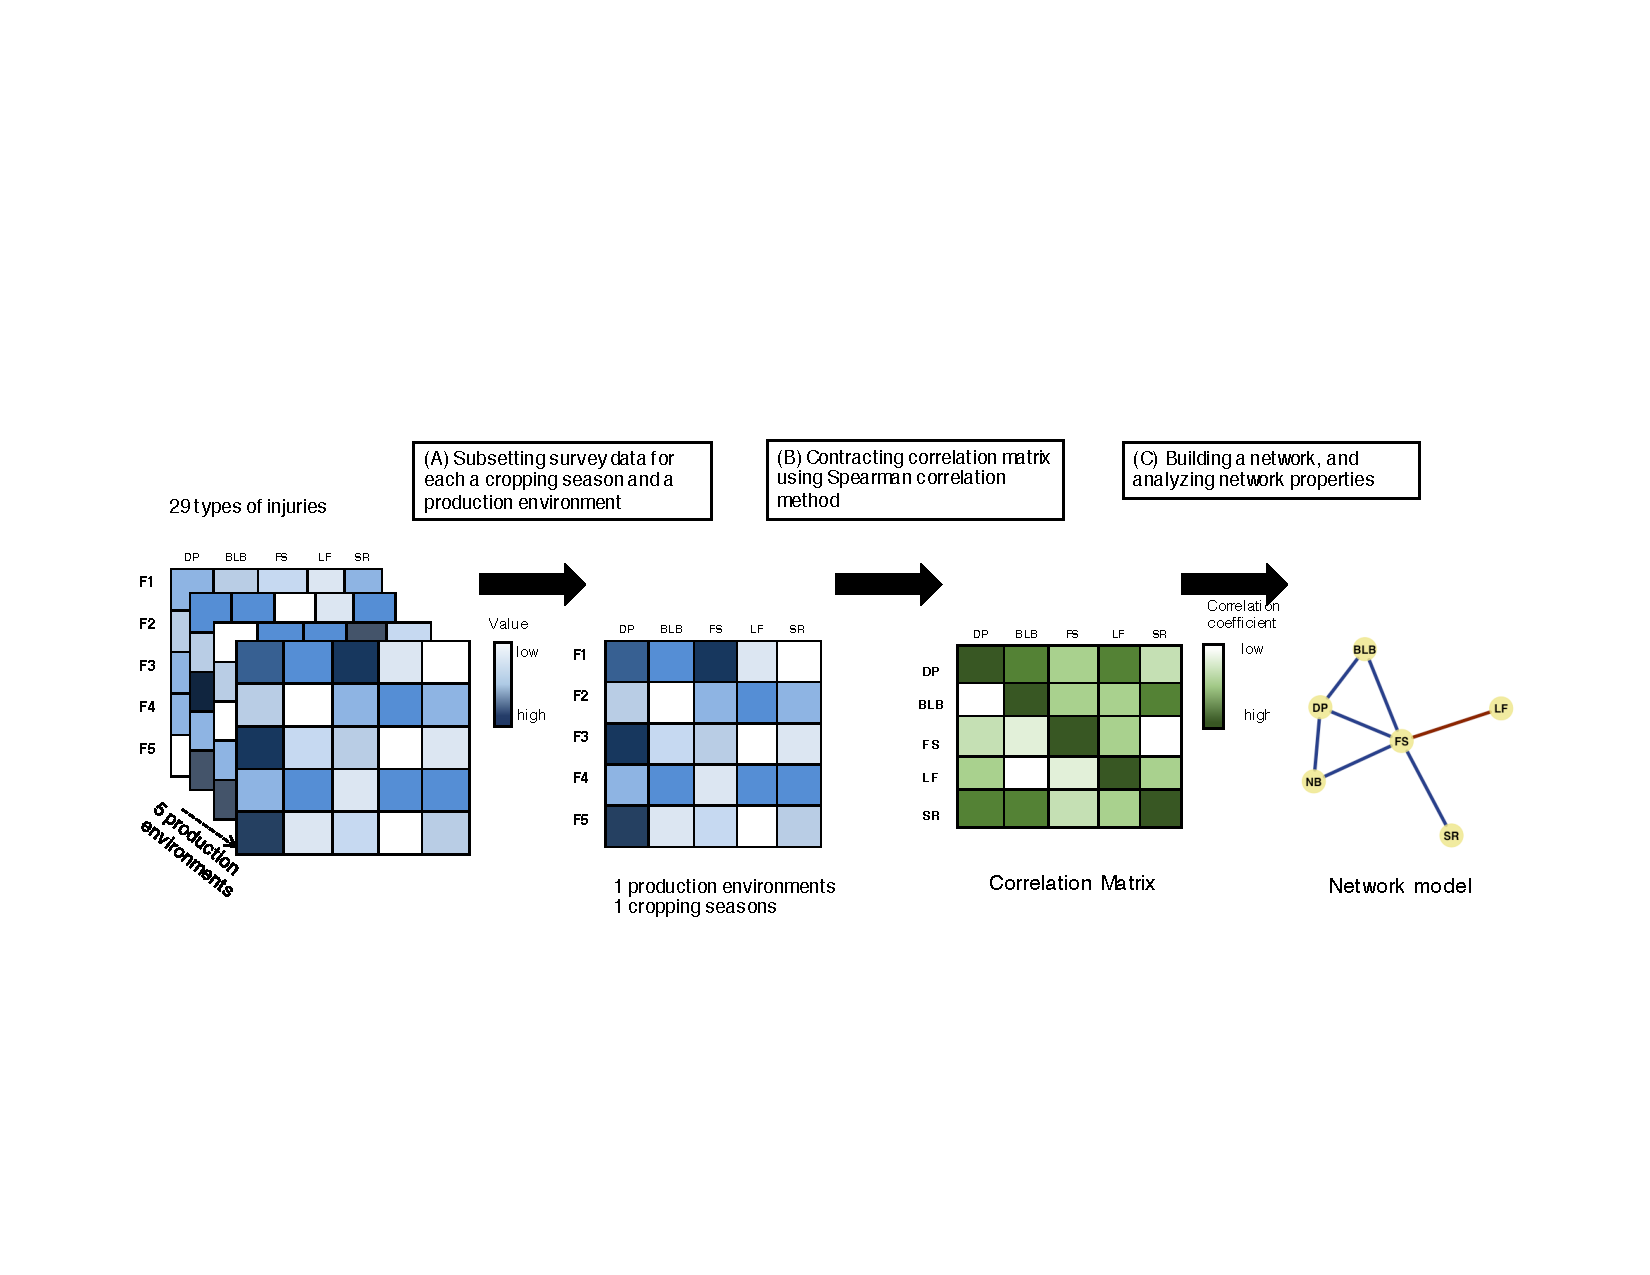
\includegraphics[width = 1\textwidth]{figures/pipeline2.pdf}
\caption[Work flow used for networks construction]{Workflow used for constructing a network that represents the co-occurrence of rice injuries based on survey data. A) subsetting survey by season, and production environment, B) constructing correlation matrix using Spearman's correlation method, and C) building network models.}
\label{fig:pipeline2}
\end{figure} 

The co-occurrence network was inferred based on adjacency matrix, which is Spearman correlation matrix constructed with \texttt{R} function \texttt{cor.test} with parameter method `Spearman' (package stats) was used for calculate Spearman's correlation coefficient ($\rho$) \citep{R_2015}.

The adjacency matrix $A$ of this network formally expresses injury occurrence, and is written in $A=[C_{ij}]$, which is

\begin{equation}
C_{ij} = \begin{cases}
C_{ij} & \text{if }  p\text{-value } < 0.05 \\ 
0 & \text{otherwise}
\end{cases}
\end{equation}

where $C$ is rank correlations coefficient ($\rho$ from the Spearman’s correlation at $p$-value < 0.05) between pairs of injures.

\begin{equation}
A = \begin{pmatrix}
0 & C_{ij}\\ 
C_{ji} & 0
\end{pmatrix}
\end{equation}

where A is the adjacency (correlation) matrix, in which the rows and column are injuries. If I ordered first by injury ($1\dots n$) and second by grid cells ($j + 1\dots n + j$), producing a square matrix with $i + j$ rows and $i + j$ columns.

From adjacency matrix, the networks were visualized with \textbf{igraph} package \citep{Csardi_2010_igraph} using indirected network and the Fruchterman–Reingold layout \citep{Fruchterman_1991_Graph}. Nodes in this network represent rice injuries and edges that connect these nodes represent correlations between injuries. 

\subsubsection{Topological feature analysis}

I calculated the topological features of each network using \textbf{igraph} package. To describe the topology of the resulted networks, a set of measures (node degree, local clustering coefficient, and betweenness) were calculated \citep{Newman_2006_Modularity}. Node degree is measured by the number of the edges (connections) of a node has. Betweenness of a node is defined by the number of of shortest paths going through a node, and the local clustering coefficients of a node is the ratio of existing edges connecting a node's neighbors to each other to the maximum possible number of such edges. The network clustering coefficient measures the degree to which nodes of the network tend to cluster together and is a measure of the connectedness of the network and is indicative of the degree of relationships in the network. 

Nodes were further classified by ranking all nodes according to three node features, partitioning this ranked list into three equally value of each node property. A node with high rank value in top third proportion of node degree, and betweenness is recognized as an indicator in co-occurrence network of rice injuries. 

\subsubsection{Community detection}

Modularity reflects the degree to which a network is organized into a modular or community structure. Modules refer to a set of nodes with denser links among them but sparser links with the rest of the network \citep{Newman_2006_Modularity}. Detection and characterization of modular structure in rice injury co-occurrence can help us to identify groups of injuries that closely related and often occur together under same situation. Several optimization algorithms are currently available, each with different advantages \citep{Brandes_2008_Modularity}. Based on the identified community structure, nodes can be grouped in terms of their roles in maintaining intra or inter-module connectivity. In this chapter, the networks were detected community structures by maximizing the modularity measure over all possible partitions by using \texttt{cluster\_optimal} function of \textbf{igraph} package. Injury nodes in the same group will be call as a syndrome, which is the combination of injuries that most likely to be observed together. 


%===========================
\newpage
\subsection{Result}

\textbf{Prevalence of injuries across sites and seasons}

Survey data were collected from farmers’ fields in five production environments (Central Plain; Thailand (CP), Odisha; India (OD), Red River Delta; Vietnam (RR), Tamil Nadu; India (TM), and West Java; Indonesia (WJ)) across South and Southeast Asia, and recorded 29 injuries caused by animal pests and pathogens.  The survey data used in this chapter were same as data analyzed in the previous chapter, which are summarized in Table \ref{table:Survey_data} and Table.\ref{table:variable_des} Prevalences of injuries a across production environments and seasons were shown in Figure.\ref{fig:barplot1} to \ref{fig:barplot3}. 

The injuries caused by animal pests observed, and recorded during the survey period were deadheart (DH), panicle mite injury (PM), leaffolder (LF), rice hispa injury (RH), whorl maggot injury (WM), whitehead(WH), rat injury (RT) rice bug injury (RB) silver shoot (SS) rice thrip injury (RTH) rice leaf miner injury (LM). These injuries were not observed at all survey fields, cropping seasons, or production environments.  DH, PM, LF, RH, WM, WH could be observed at all season and production environment. However, they had different levels of prevalence. For example, PM could be observed higher in RR than other production environments, and RT presented at all location too, but heavily at WJ. Some injuries were not reported in production environments. SS, RTH, and LM were not presented in RR, OD, and TM, respectively. RB were reported heavily in WJ, but not in other production environments.  
 
Rice diseases recorded were bacterial leaf blight (BLB), bacterial leaf streak (BLS), brown spot (BS), leaf blast (LB), narrow brown spot (NBS), read stripe (RS), sheath blight (SHB), sheath rot (SR), false smut (FS), stem rot (SR). Diseases observed in this study were commonly found at all locations, but there were some diseases that could not be observed. DP seem to appear at all location, except in Odisha, this disease tended to occur in wet season, more than dry season in CP and RR. Conversely, in TM and WJ, dirty panicle prevailed higher in dry season than wet season. FS presented at all location. They are high prevalence especially in OR, and TM.  BLS, LS were not reported in OD and TM. The diseases observed at all location were BS, NB, LB, SHB, SHR with different degree of prevalence.  BS prevailed highly in CP, LB had high prevalence in OD, and SHR and NBS highly occurred in CP and WJ. RS were found heavily in CP, but a few in WJ and not reported in OD, RR, TM.

Systemic injuries in this survey include hopper burn (HB) caused by brown plant hoppers, and white backed plant hoppers, bug burn (BB) caused by rice black bugs, and three viral diseases; rice grassy stunt (GS), ragged stunt (RGS), and tungro (RTG). HB could be commonly found at all production environments.  A few locations in CP, RR and WJ were observed BB. GS were reported in RR and WJ. RGS were not reported in OR and RR, and RTG were reported only in WJ.

    \begin{landscape}
\begin{figure}
\centering
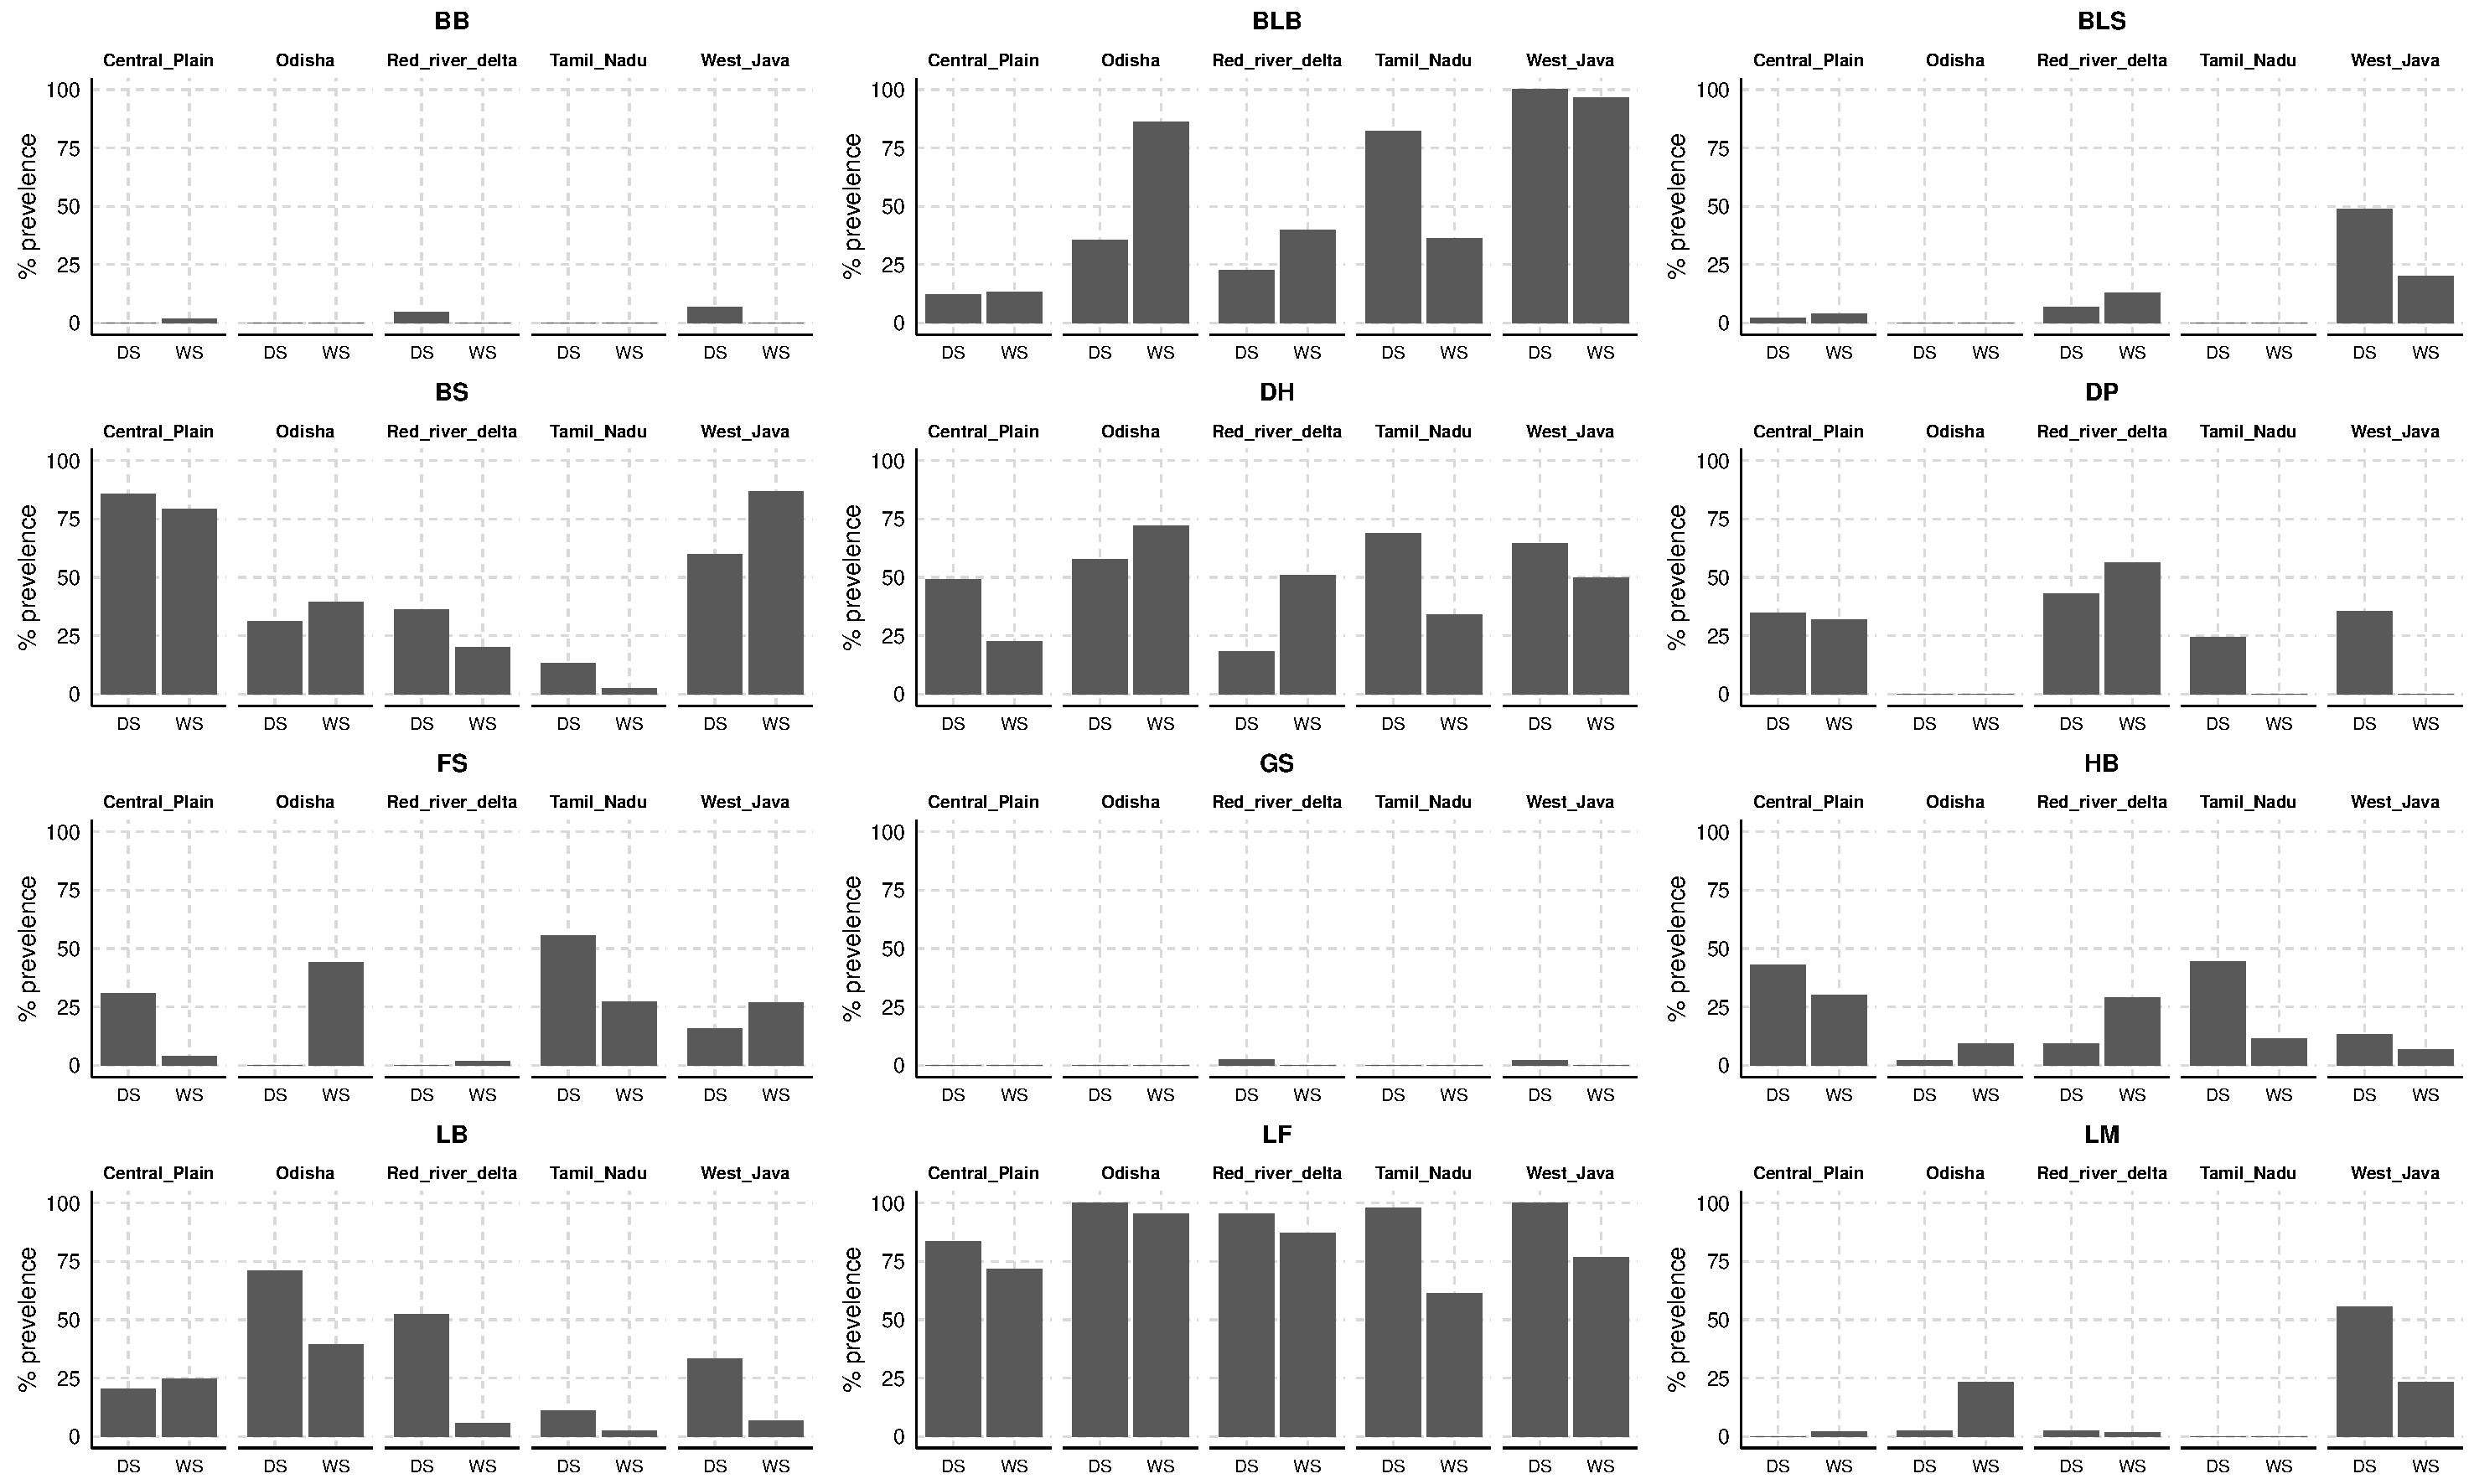
\includegraphics[height = 1\textwidth]{figures/barplot1.pdf}
\caption[Bar graphs showing  prevalence of injuries a across production environments and seasons.]{Bar graphs showing  prevalence of injuries a across production environments and seasons. BB: Bugburn, BLB: Bacterial leaf blight, BLS: Bacterial leaf streak, BS: Brown spot, DH: Deadheart, DP: Dirty panicle, FS: False smut, GS: Grassy stunt, HB: Hopperburn, LB: Leaf blast, LF: Leaffolder injury, LM: Leaf miner injury, LS: :Leaf scald, NB: Neck blast, NBS:  Narrow brown spot, PM: Panicle mite injury, RB: Rice bug injuries, RGS: Ragged stunt, RH: Rice hispa injury, RS: Red stripe, RT: Rat injury, RTG: Tungro, RTH: Rice thrip injury, SHB: Sheath blight, SHR: Sheath rot, SR: Stem rot, SS: Silver shoot, WH: Whitehead, WM: Whorl maggot injury.}
\label{fig:barplot1}
\end{figure}    
\end{landscape} 
    
 \begin{landscape}
\begin{figure}
\centering
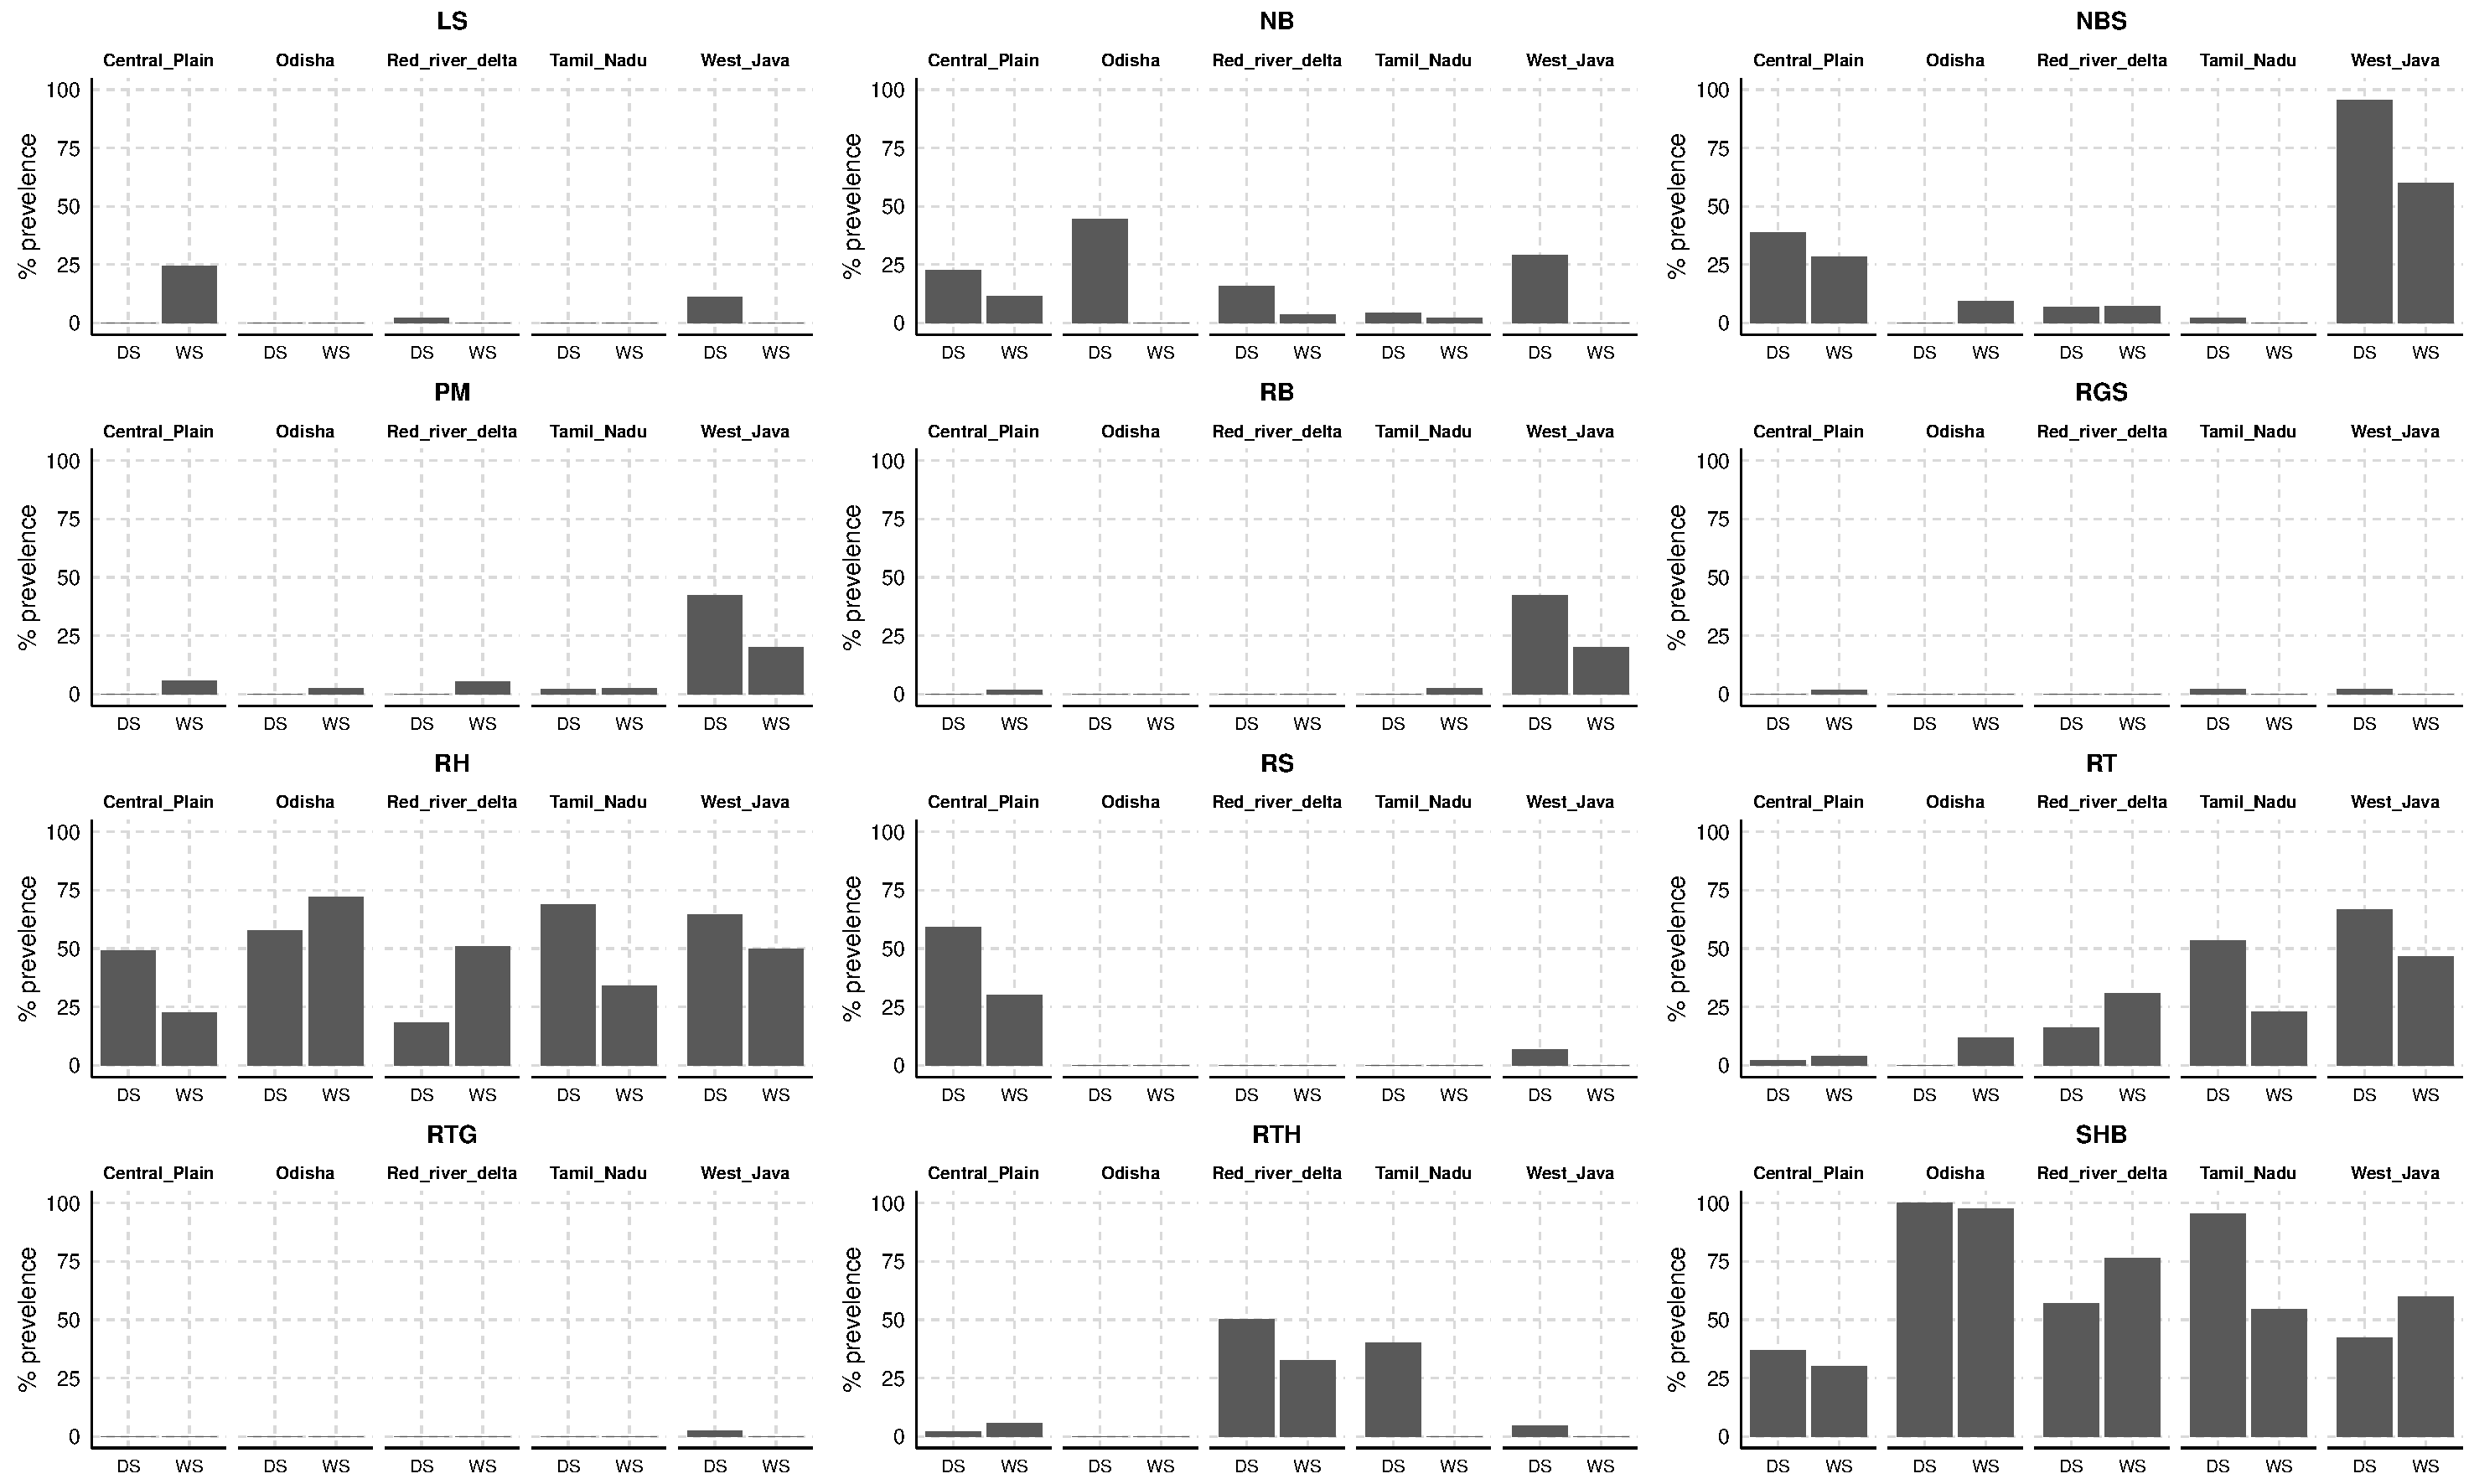
\includegraphics[height = 1\textwidth]{figures/barplot2.pdf}
\caption[\textit{Continue}]{(\textit{Continue}) Bar graphs showing  prevalence of injuries a across production environments and seasons.}
\label{fig:barplot2}
\end{figure}\end{landscape} 

    
    \begin{landscape}
\begin{figure}\
centering
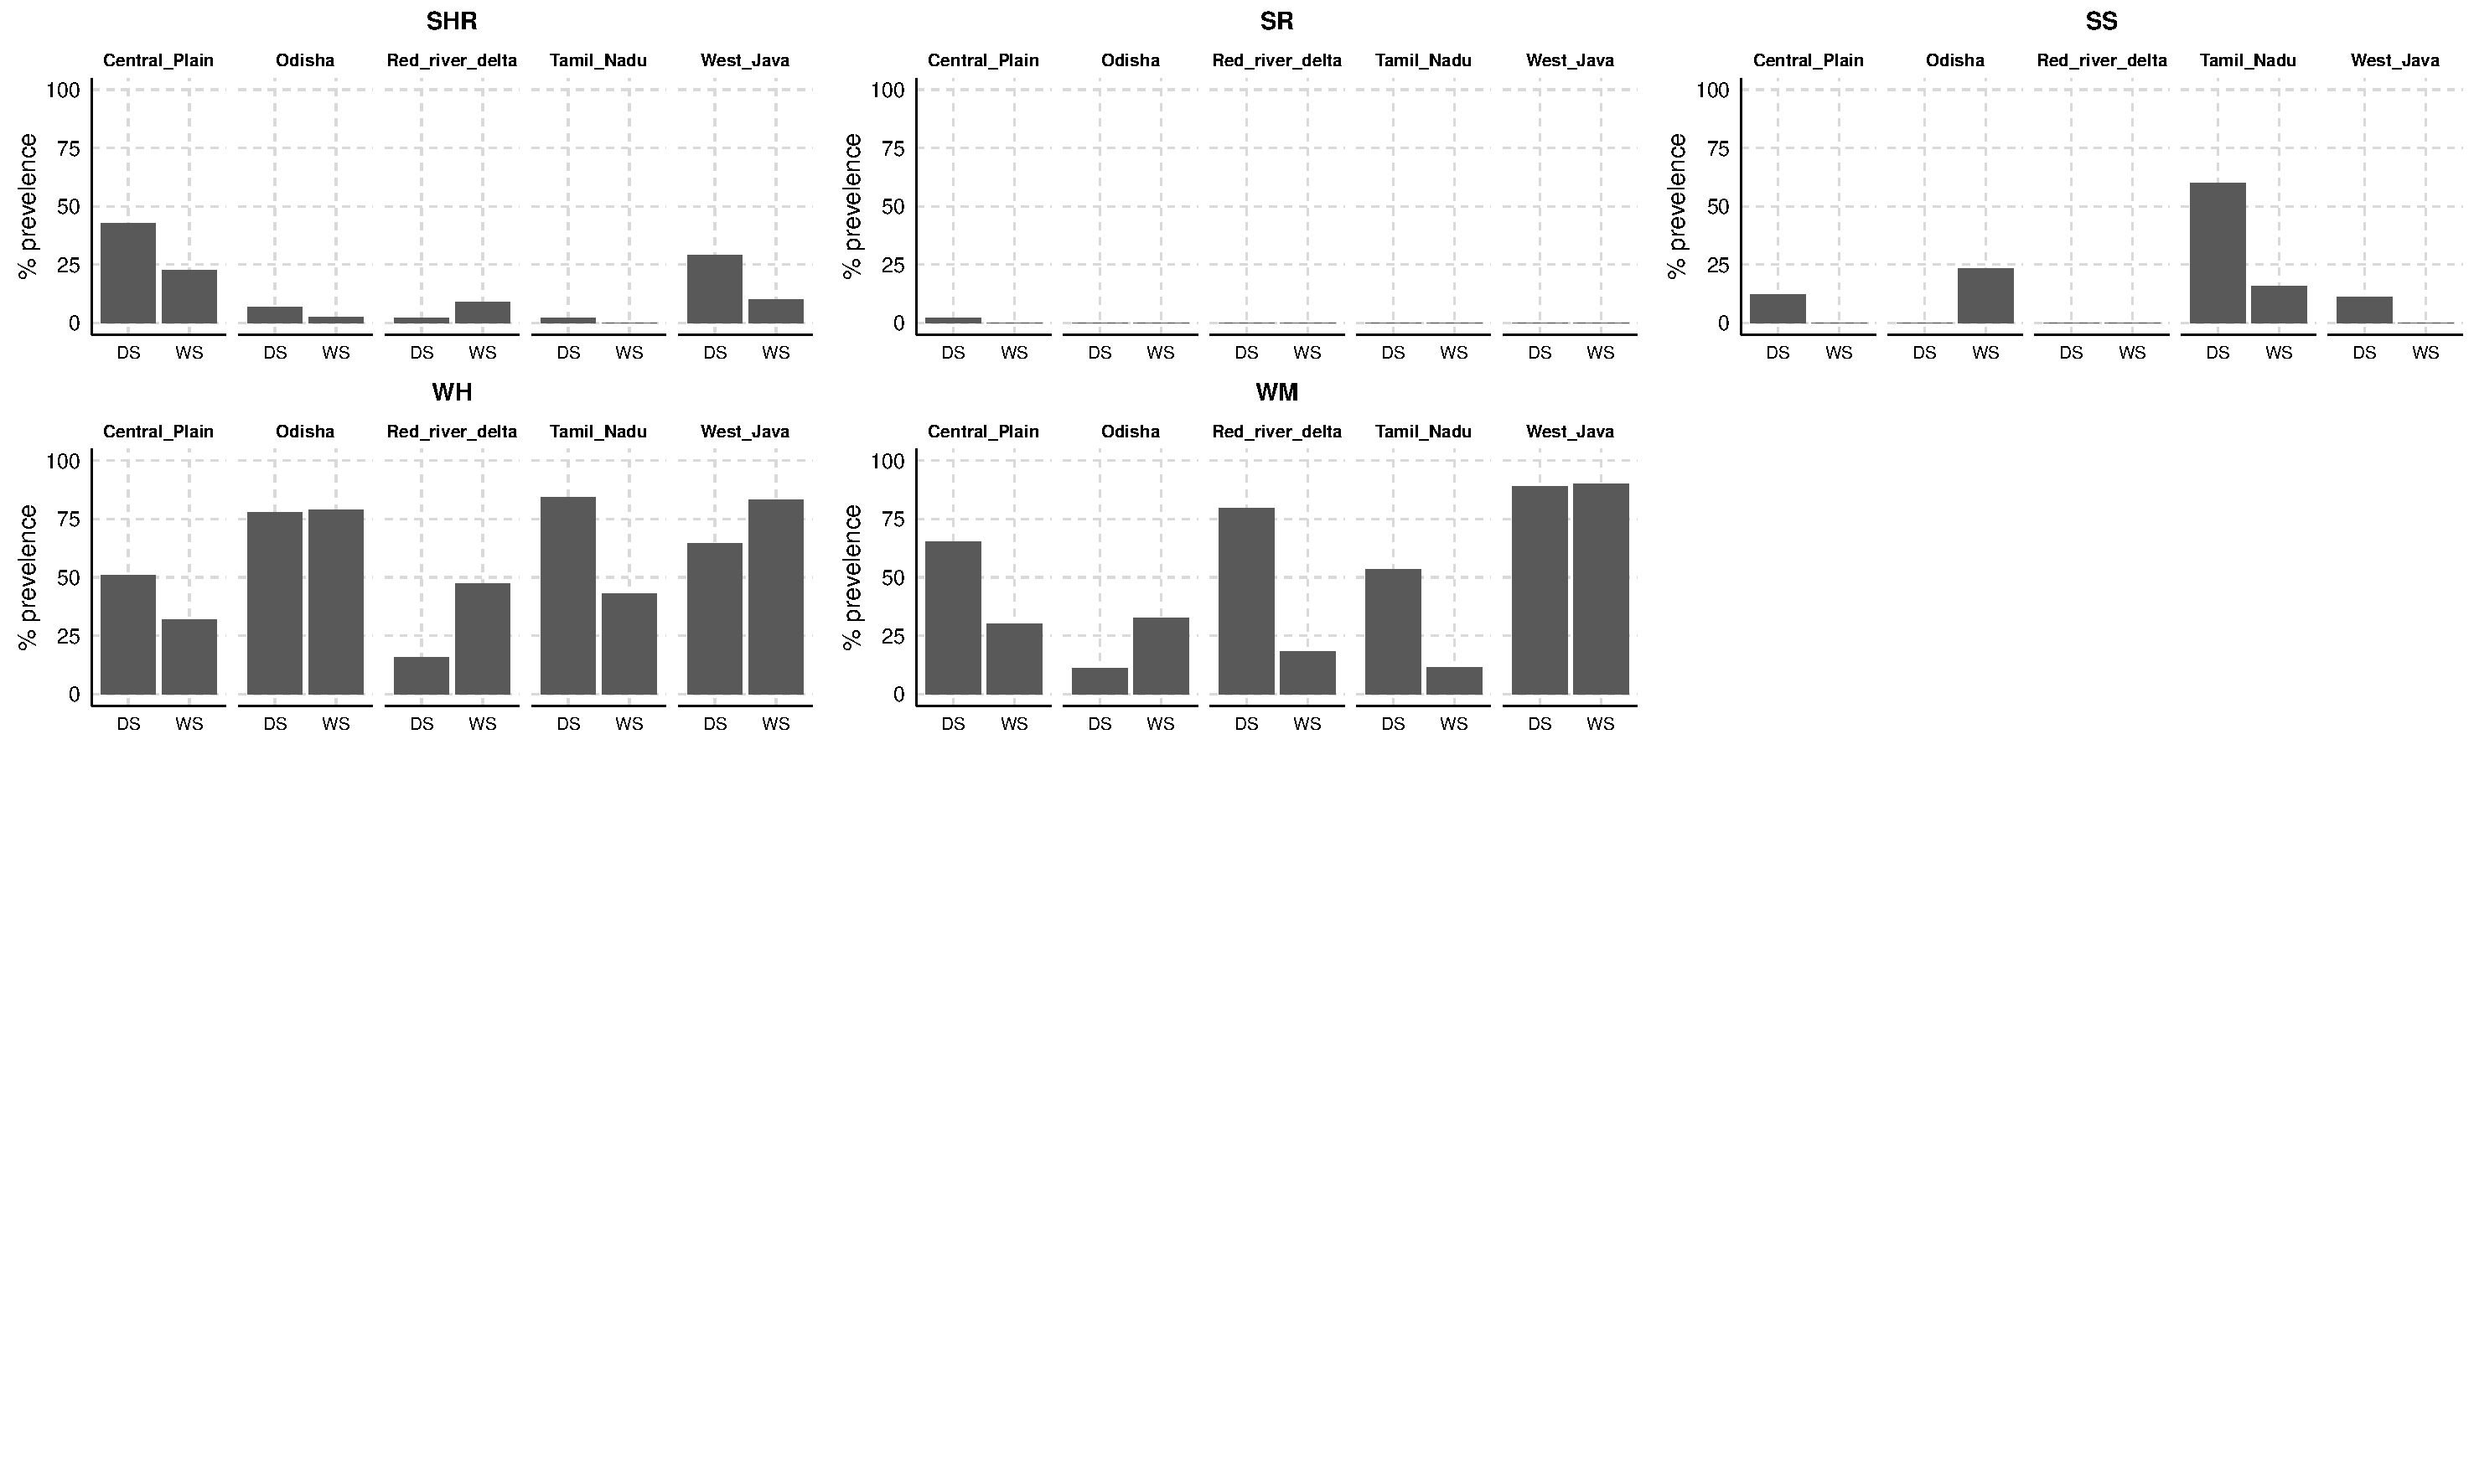
\includegraphics[height = 1\textwidth]{figures/barplot3.pdf}
\caption[\textit{Continue}]{(\textit{Continue}) Bar graphs showing  prevalence of rice injuries across production environments and seasons.} 
\label{fig:barplot3} 
\end{figure}  
\end{landscape} 


\subsubsection{Structures, compositions, and communities of co-occurrence network of rice pest injuries}

The co-occurrence networks for crop health data are given in Figure. \ref{fig:CP_ds} to Figure \ref{fig:WJ_ws}. To analyze the rice injury network, I focus on the most prominent properties of nodes in a network node: node strength, betweenness, and clustering coefficient. Node strength is a measure of the number of connections a node has, weighted by Spearman’s correlation coefficient. Betweenness measures how often a node lies on the shortest path between every combination of two other nodes, indicating how important the node is in the flow of information through the network \citep{Opsahl_2010_Node}. The local clustering coefficient is a measure of the degree to which nodes tend to cluster together. It is defined as how often a node forms a triangle with its direct neighbors, proportional to the number of potential triangles the relevant node can form with its direct neighbors \citet{Opsahl_2010_Node}. These measures are indicative of the potential association activity through the network. As activated injuries can activate other injuries, a more densely connected network facilitates injury occurrence. Moreover, the community structure of the networks derived from the empirical data can be inspected to identify syndromes (clusters of injuries) that are especially highly associated.
%\begin{table}
\centering
\label{table:network_prop}
\begin{tabular}{llllll}
\hline
Production environment   & Season & Node & Edges & Average short path & Clustering coefficient \\
\hline
Central Plain, Thailand  & Dry    & 18   & 60    & 1.96               & 0.75                   \\
Central Plain, Thailand  & Wet    & 20   & 48    & 2.79               & 0.65                   \\
Odisha, India            & Dry    & 9    & 13    & 1.19               & 0.89                   \\
Odisha, India            & Wet    & 15   & 26    & 2.14               & 0.66                   \\
Red River Delta, Vietnam & Dry    & 19   & 26    & 2.15               & 0.58                   \\
Red River Delta, Vietnam & Wet    & 18   & 37    & 2.00               & 0.52                   \\
Tamil Nadu, India        & Dry    & 16   & 31    & 2.02               & 0.73                   \\
Tamil Nadu, India        & Wet    & 12   & 30    & 1.67               & 0.67                   \\
West Java, Indonesia     & Dry    & 26   & 99    & 2.14               & 0.56                   \\
West Java, Indonesia     & Wet    & 14   & 18    & 1.39               & 0.69                   \\
\hline
\end{tabular}
\end{table}

%Microbial communities show significant higher interaction strength among positive interactions (i.e. potential mutualistic; SPF: W = 489396, P < 2.20 × 10−16; Wilcoxon test). However, the higher frequency of negative weak interactions overall has a stabilizing effect preventing the communities from collapsing (positive/ negative interactions = 0.482; # P < 0.100, * P < 0.050, ** P < 0.010, *** P < 0.001).


% I will use this for discuss the anti-cooccurence realtionships

%Network  suggested that co-occurrences of mutated genes in cancers were more abundant than anti-co-occurrences; although this finding generally held true in our study, the importance of anti-co-occurrences was underestimated. We found that the high-frequent genes, i.e., those that were mostly frequently mutated in cancers, were often involved in the CCA network and tended to anti-co-occur with other genes. Significant co- occurrences were indeed the most abundant, but they often occurred in genes that were mutated in a small number of cancer samples. For example, we found 76 pairs of significant co-occurrences and anti-co-occurrences in cancer samples of the urinary tract. Of those, 79\% were co-occurrences (Fig. 3; green lines), and only 21\% were anti-co-occurrences (Fig. 3; red lines). In addition, all of the top five most frequently mutated genes (hereafter referred to as ‘high-frequent genes’; colored nodes) were involved in the CCA network, and the anti-co-occurrences among them and between them and other genes (grey nodes) were significantly enriched (p 1⁄4 0.04, Odds Ratio (OR) 1⁄4 3.19; Fisher's Exact Test (FET)). Similar results could be found in samples that originated from other tissues such as hematopoietic and lymphoid tissue (p 1⁄4 0.04, OR 1⁄4 3.19; FET), as shown in Fig. 4 as well as the central nervous system (Fig. S1) and breast (Fig. S2). Overall, among the 19 tissues (primary histology sites) of cancer samples that were collected in COSMIC, none showed enrichment of co-occurrences in the top five high-frequent genes. As shown in Figs. 3 and 4, the genes that are less frequently mutated in cancer samples (grey nodes) tend to be co-mutated (connected with green edges).

\textbf{Central Plain, Thailand}

\begin{figure}
   \begin{subfigure}[b]{0.5\textwidth}
        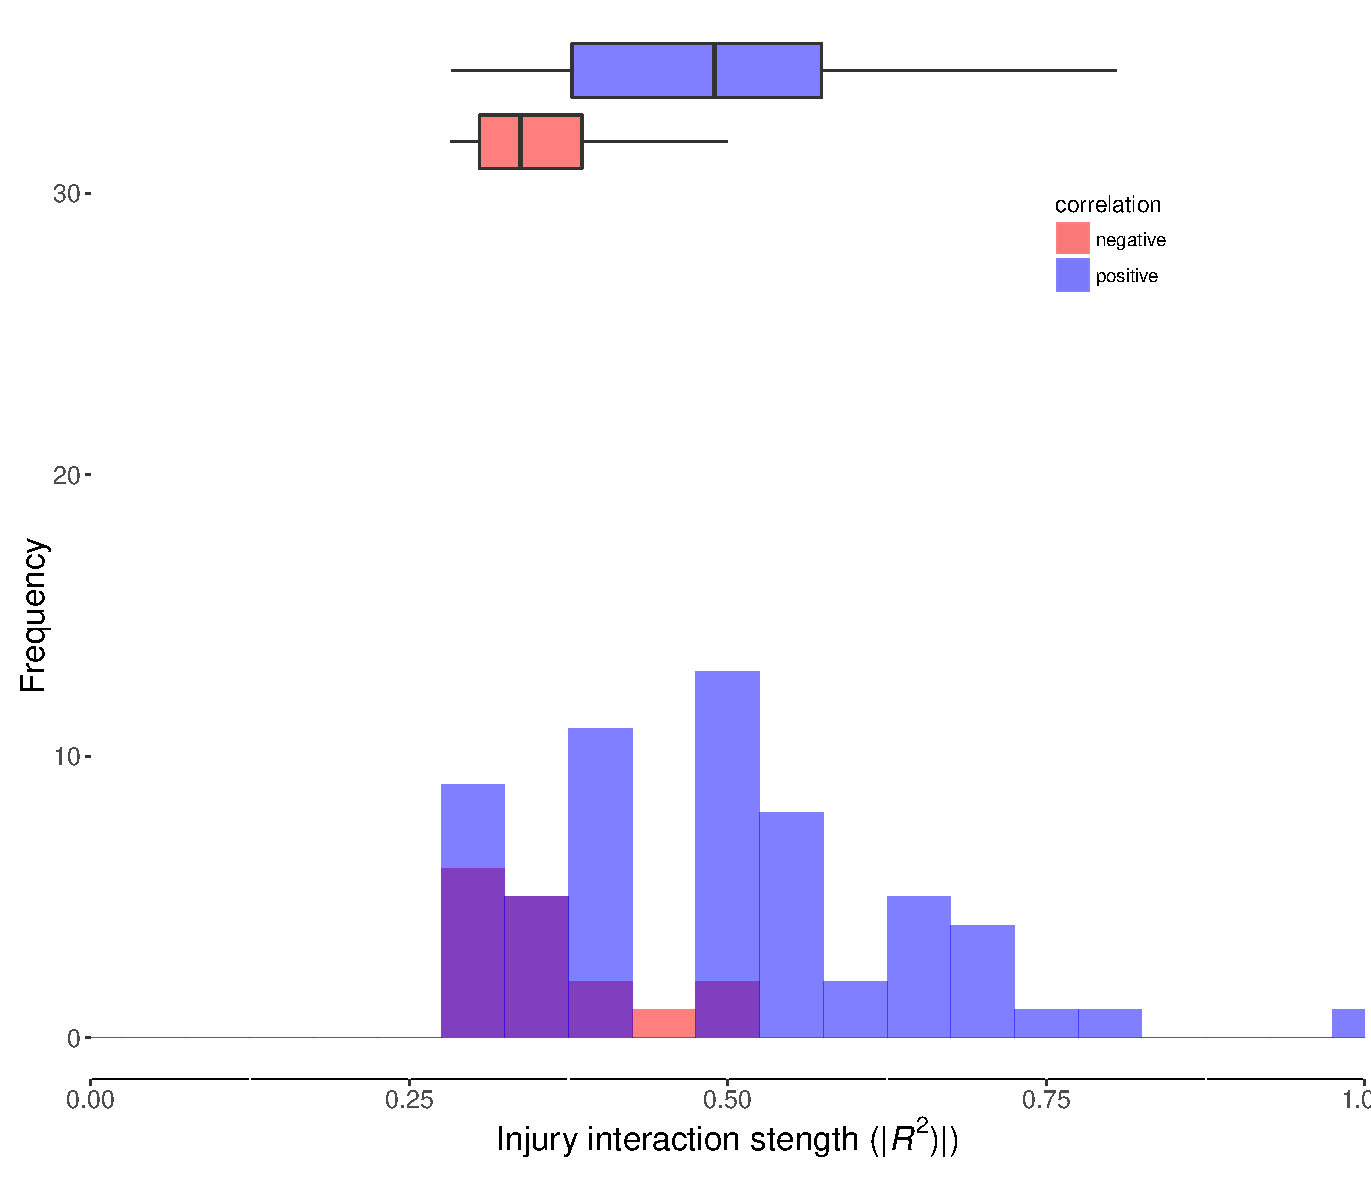
\includegraphics[width = \textwidth]{figures/combinedplotCP_ds.pdf}
        \caption{Distribution of pairwise injury correlations in survey data in dry season at Central Plain}
        \label{fig:}
    \end{subfigure}
    \begin{subfigure}[b]{0.5\textwidth}
        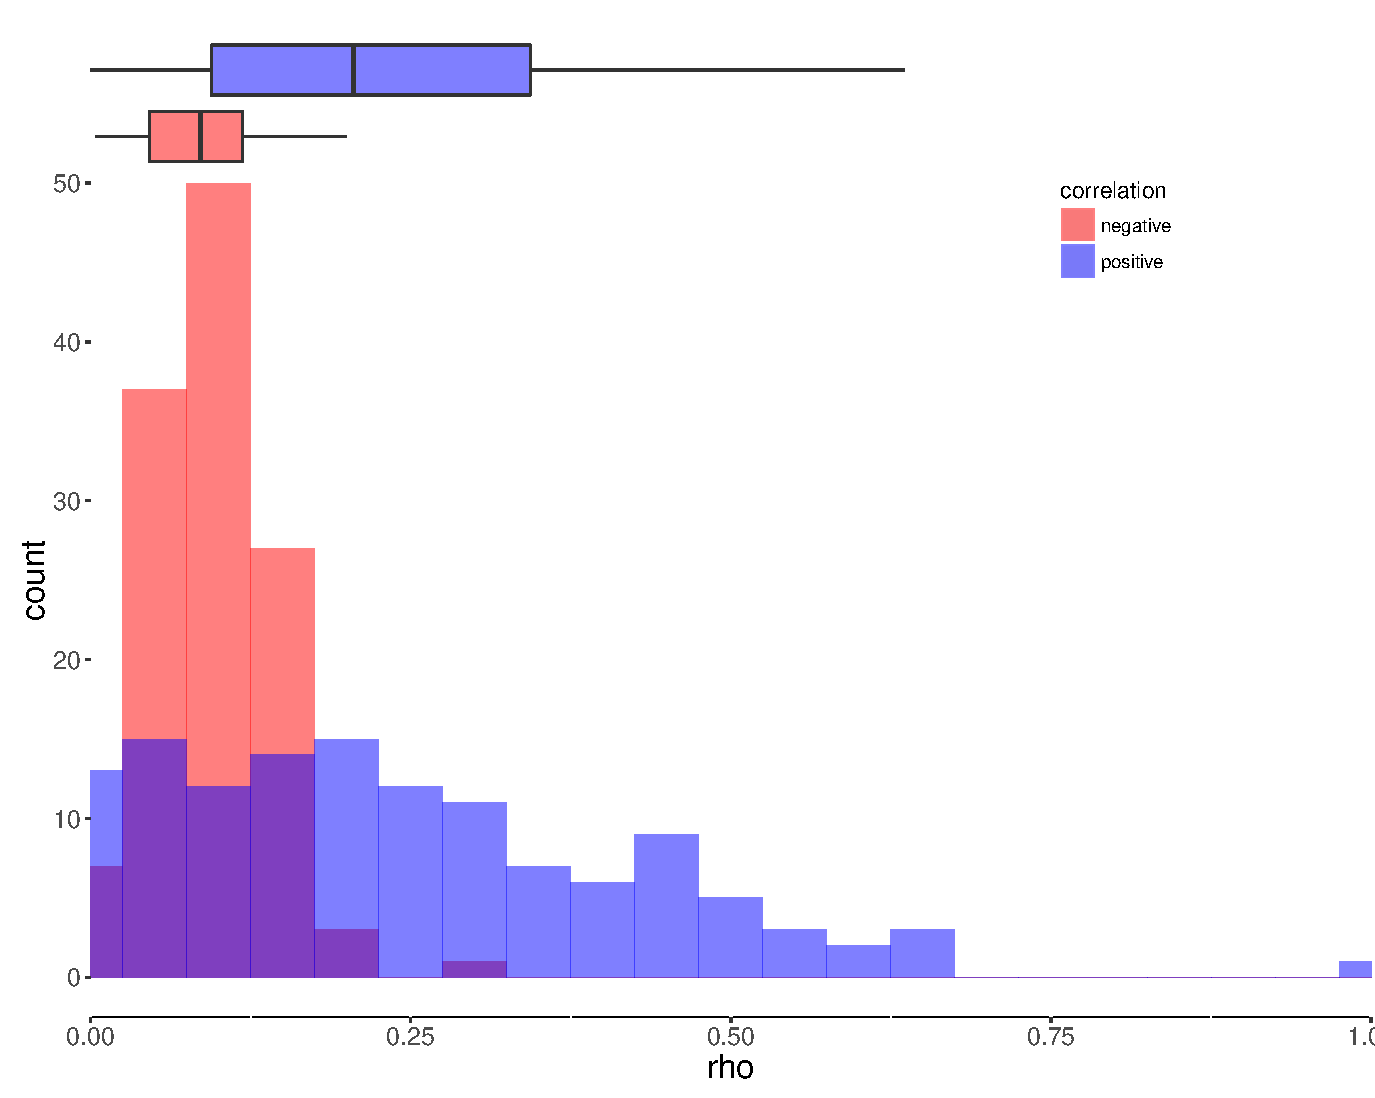
\includegraphics[width = \textwidth]{figures/combinedplotCP_ws.pdf}
        \caption{Distribution of pairwise injury correlations in survey data in wet season at Central Plain}
        \label{fig:.}
    \end{subfigure}
\begin{subfigure}[b]{0.4\textwidth}
        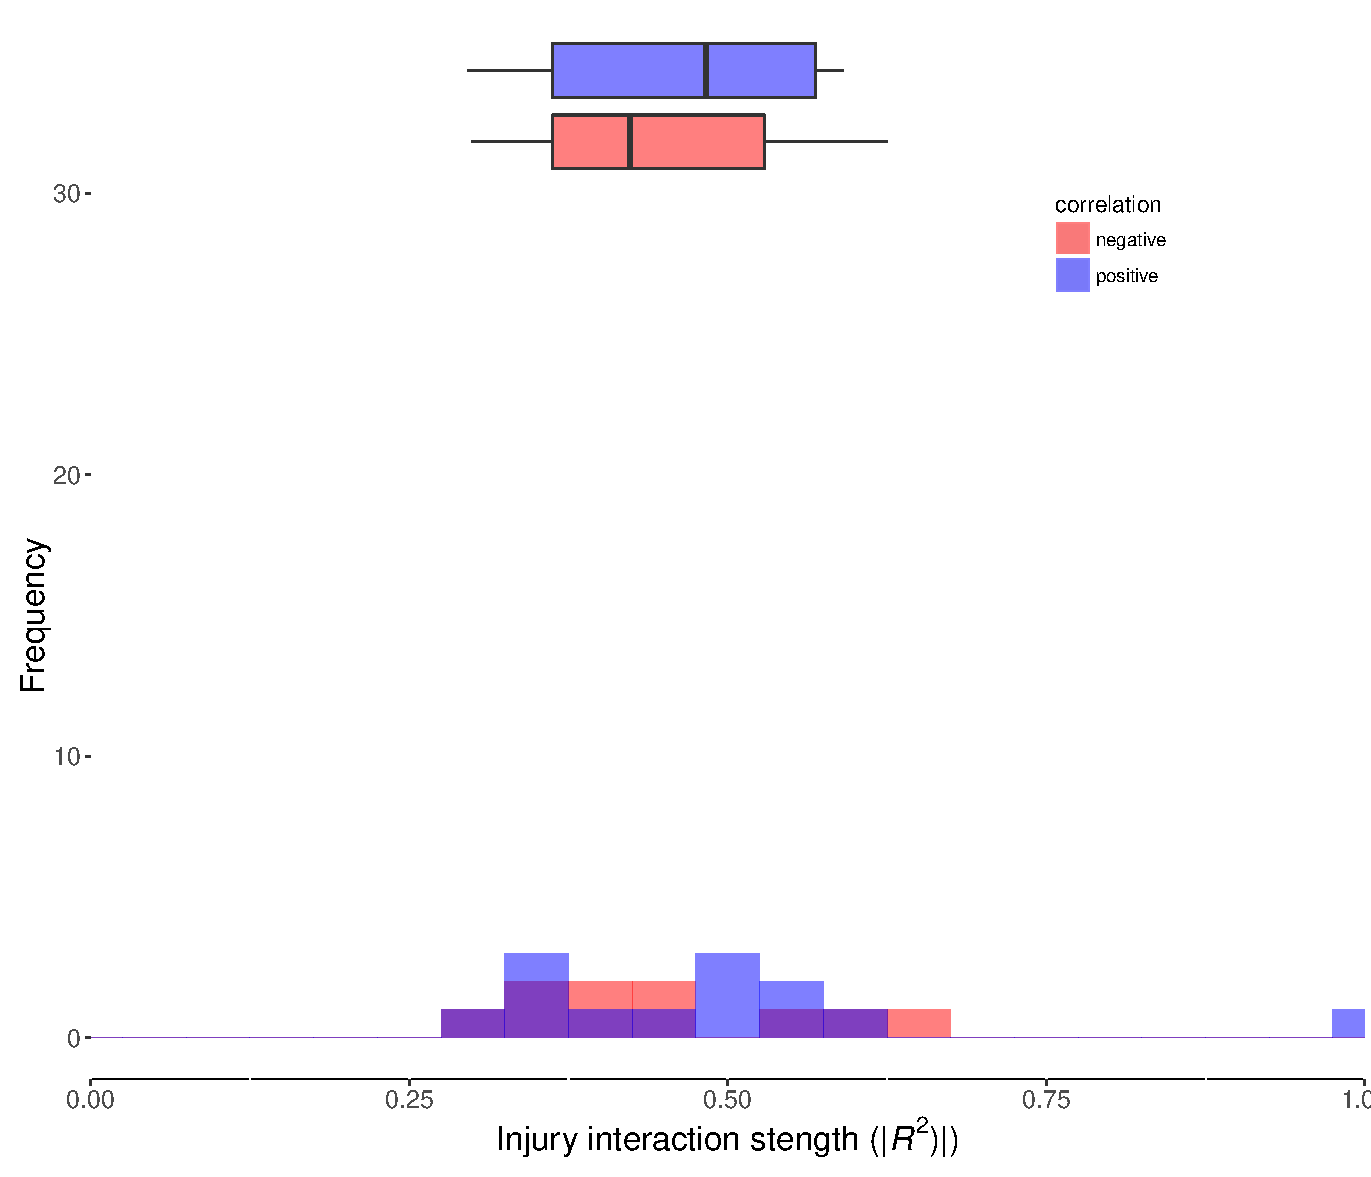
\includegraphics[width = 1\textwidth]{figures/combinedplotOD_ds.pdf}
        \caption{.s.}
        \label{fig:.}
    \end{subfigure}
\begin{subfigure}[b]{0.4\textwidth}
        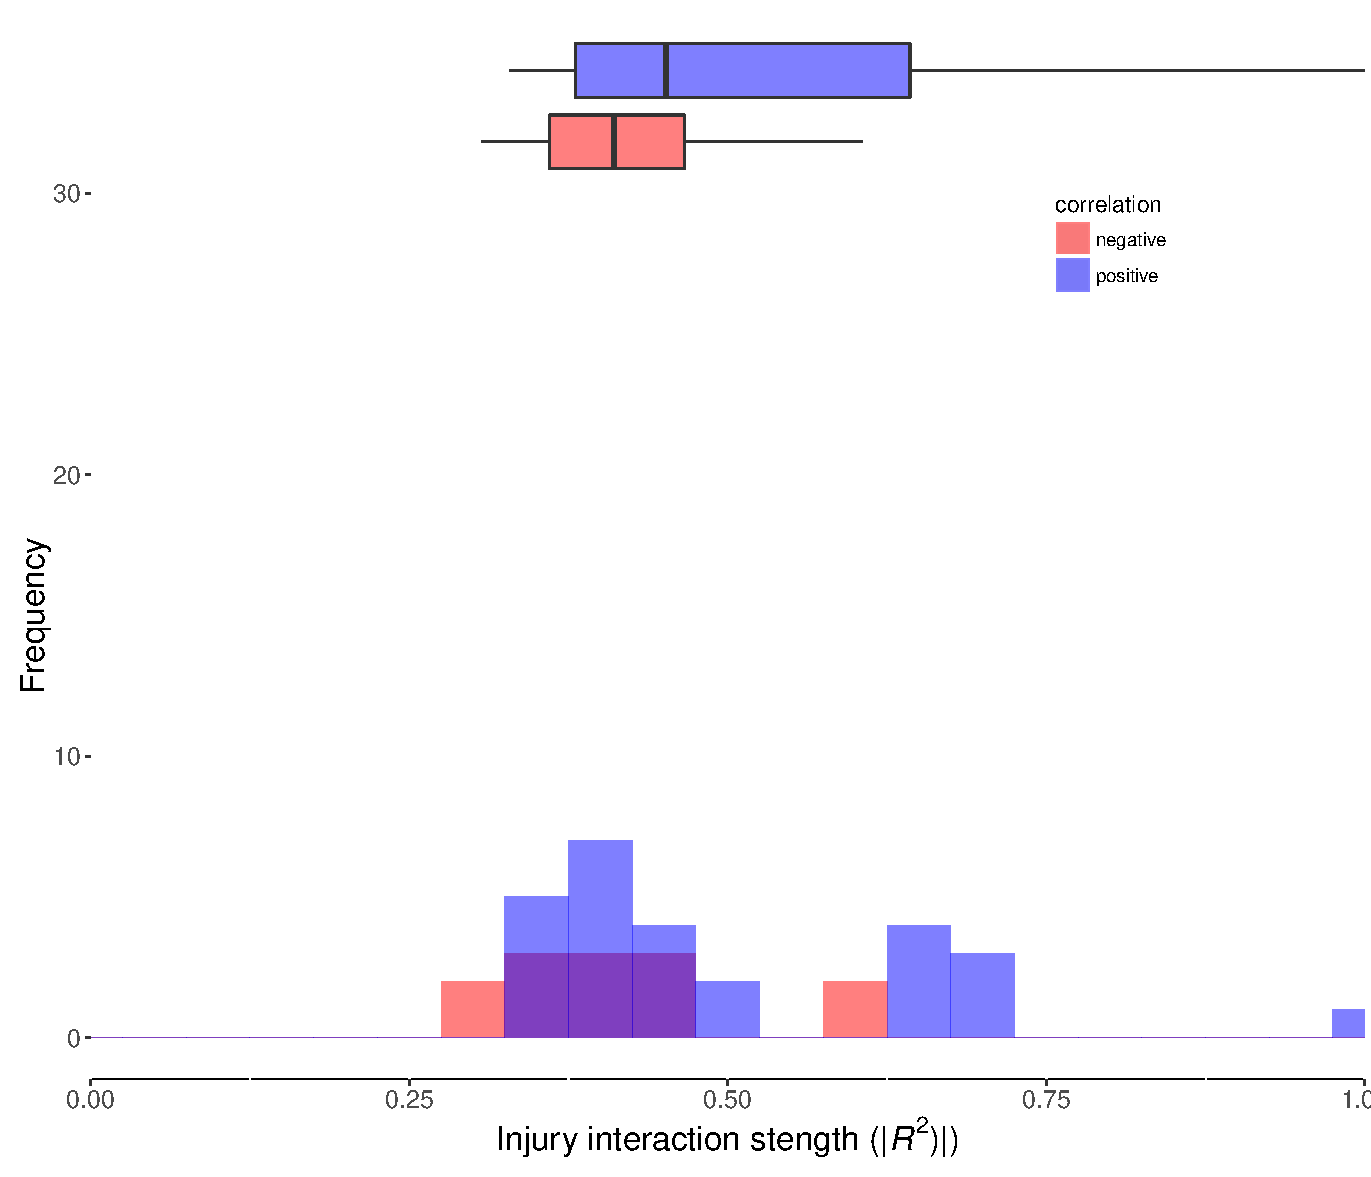
\includegraphics[width = 1\textwidth]{figures/combinedplotOD_ws.pdf}
        \caption{.s.}
        \label{fig:.}
    \end{subfigure}
\begin{subfigure}[b]{0.4\textwidth}
        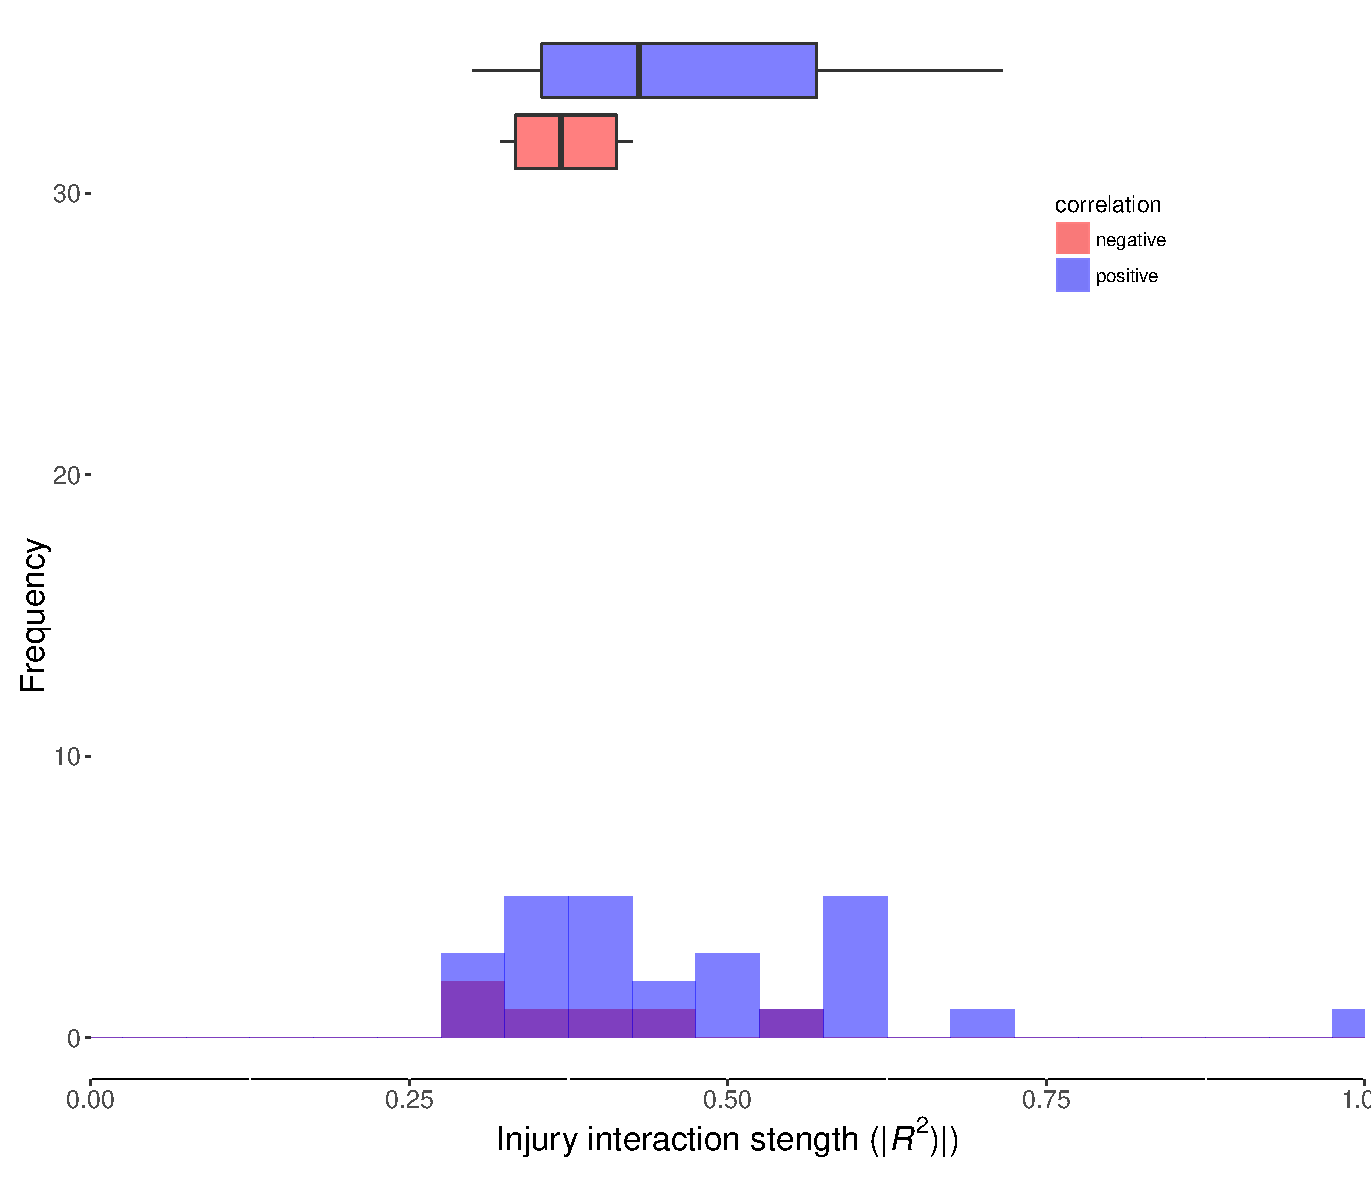
\includegraphics[width = 1\textwidth]{figures/combinedplotRR_ds.pdf}
        \caption{.s.}
        \label{fig:.}
    \end{subfigure}
\begin{subfigure}[b]{0.4\textwidth}
        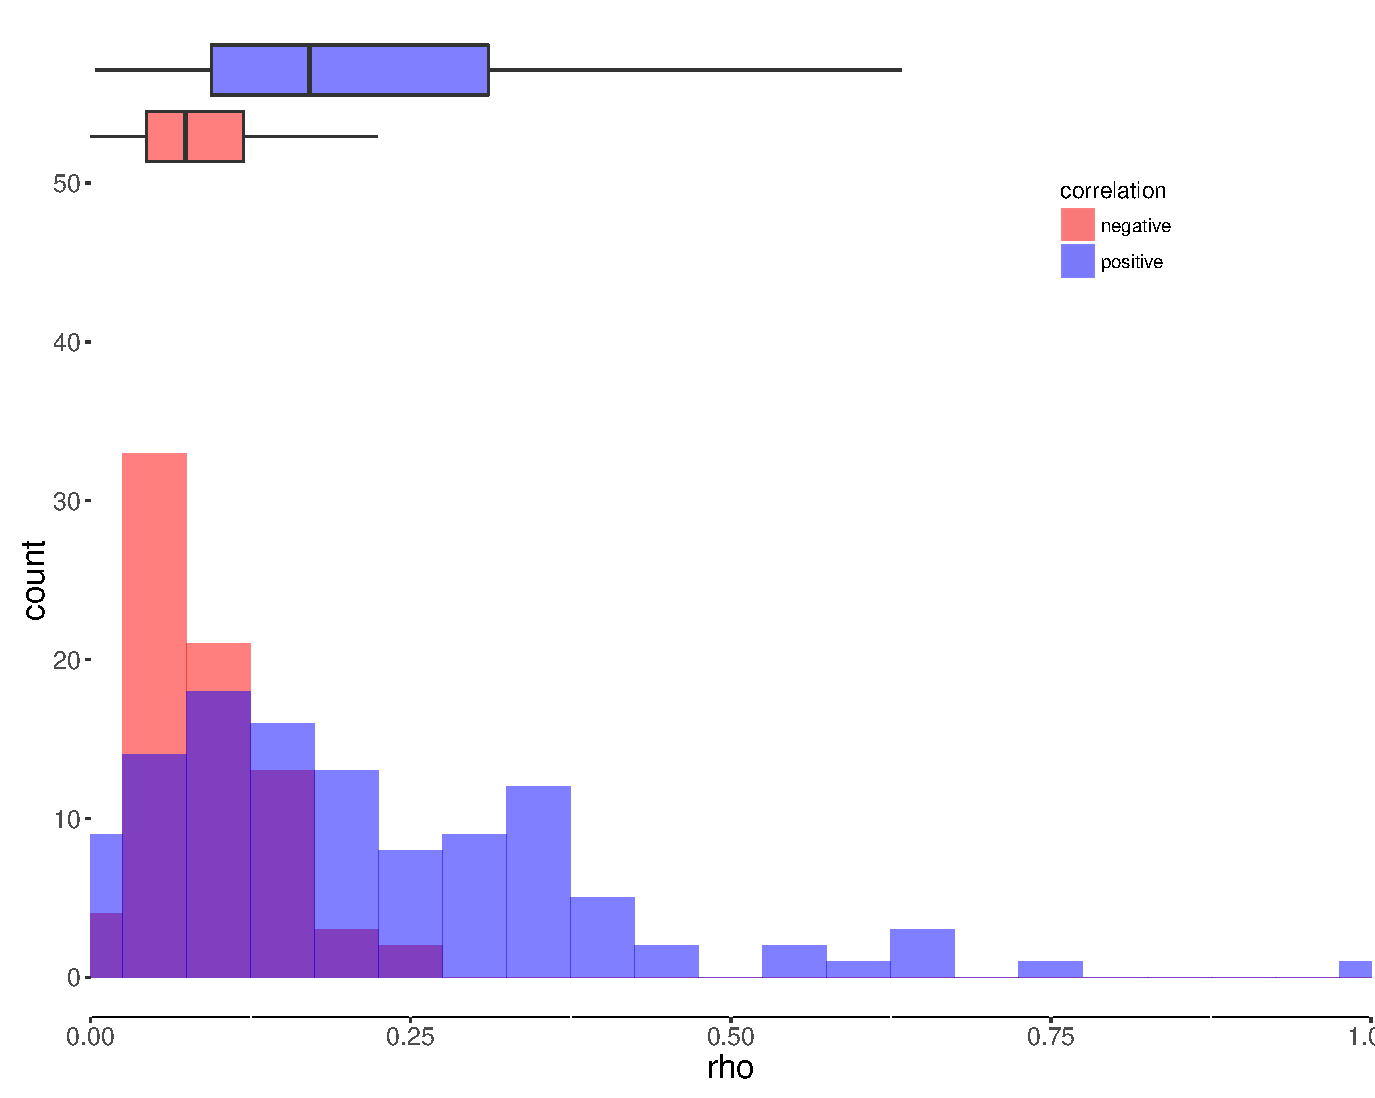
\includegraphics[width = 1\textwidth]{figures/combinedplotRR_ws.pdf}
        \caption{.s.}
        \label{fig:.}
    \end{subfigure}
\begin{subfigure}[b]{0.4\textwidth}
        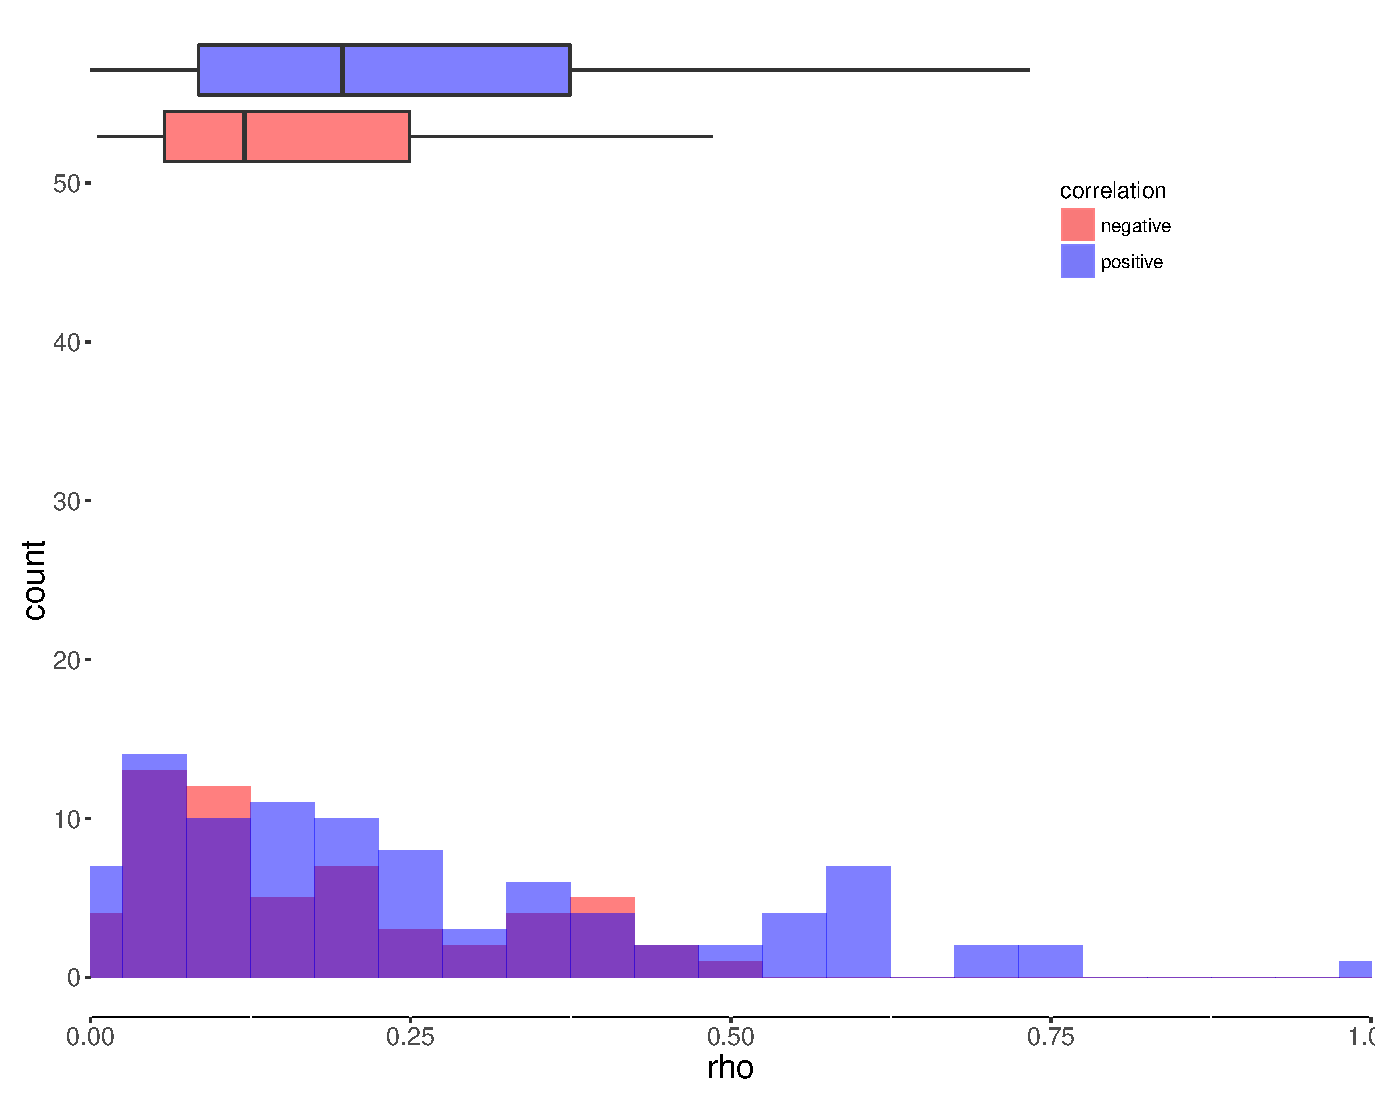
\includegraphics[width = 1\textwidth]{figures/combinedplotTM_ds.pdf}
        \caption{.s.}
        \label{fig:.}
    \end{subfigure}
\begin{subfigure}[b]{0.4\textwidth}
        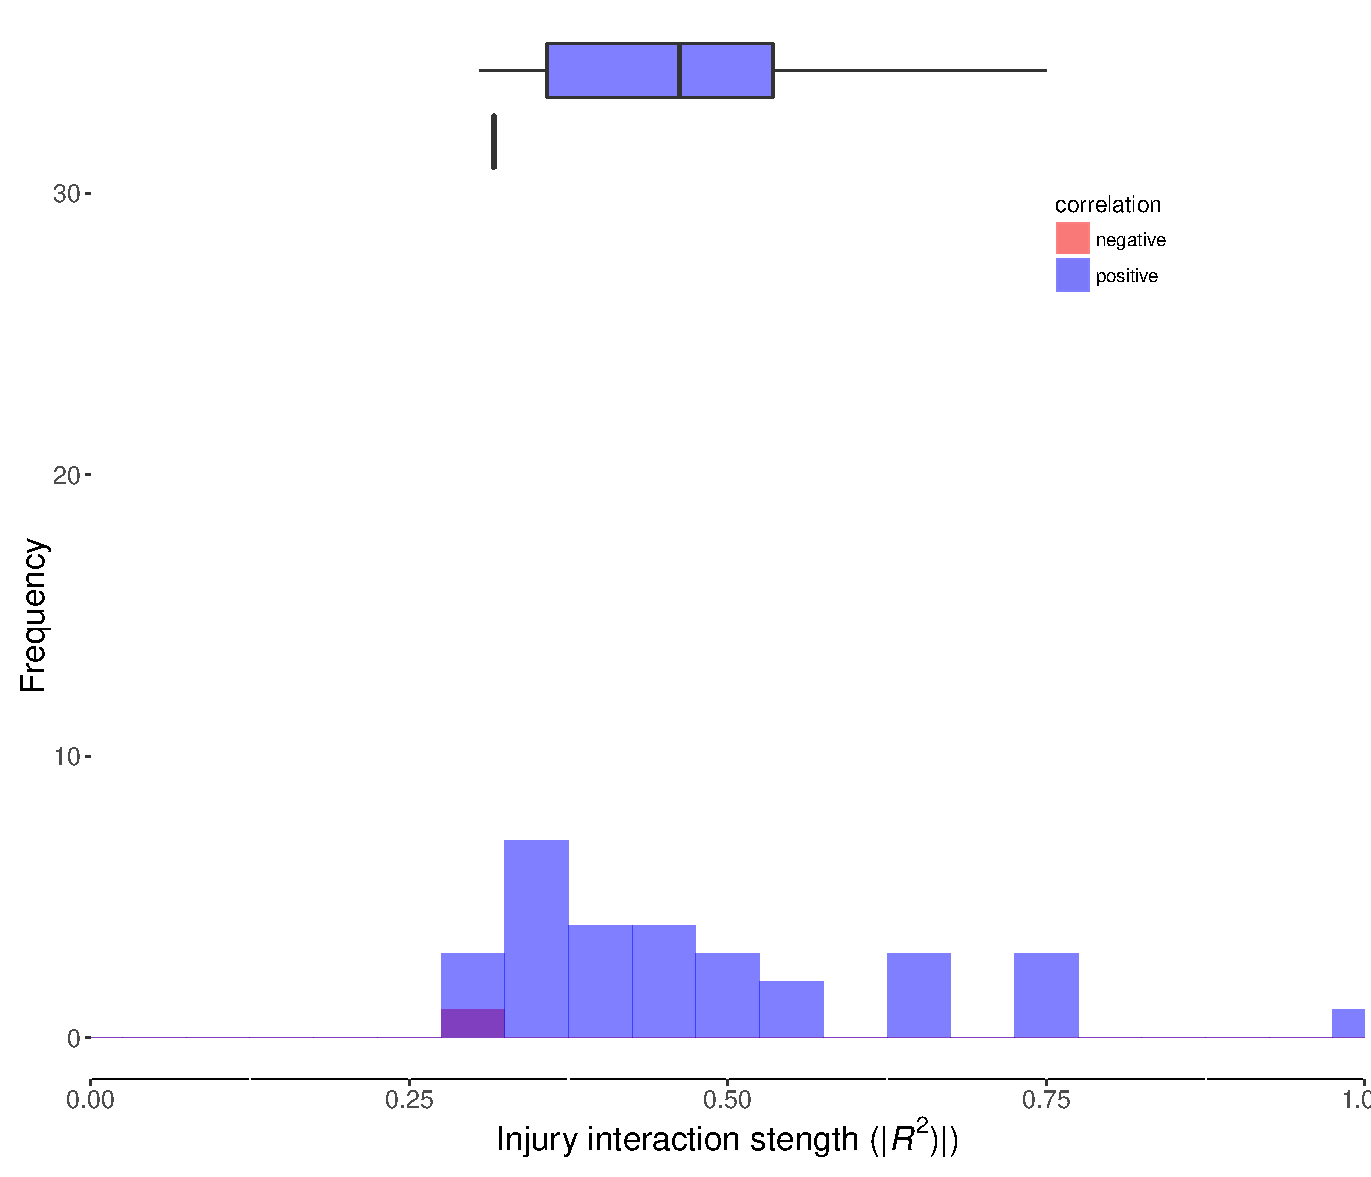
\includegraphics[width = 1\textwidth]{figures/combinedplotTM_ws.pdf}
        \caption{.s.}
        \label{fig:.}
    \end{subfigure}
\begin{subfigure}[b]{0.4\textwidth}
        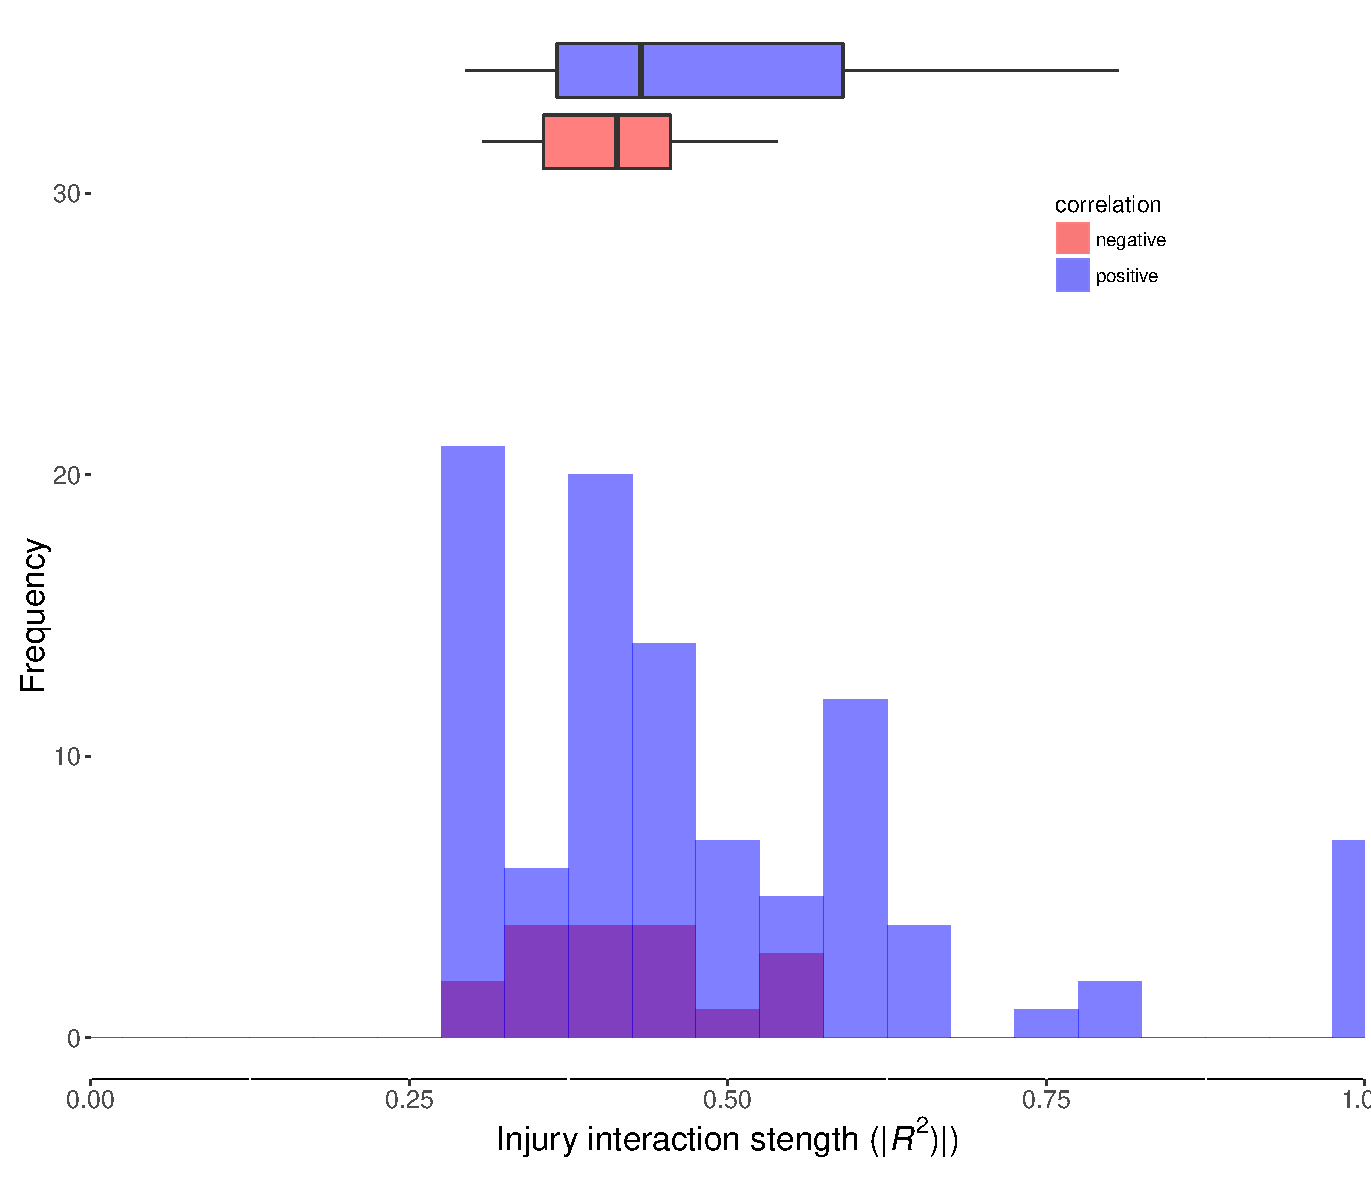
\includegraphics[width = 1\textwidth]{figures/combinedplotWJ_ds.pdf}
        \caption{.s.}
        \label{fig:.}
    \end{subfigure}
\begin{subfigure}[b]{0.4\textwidth}
        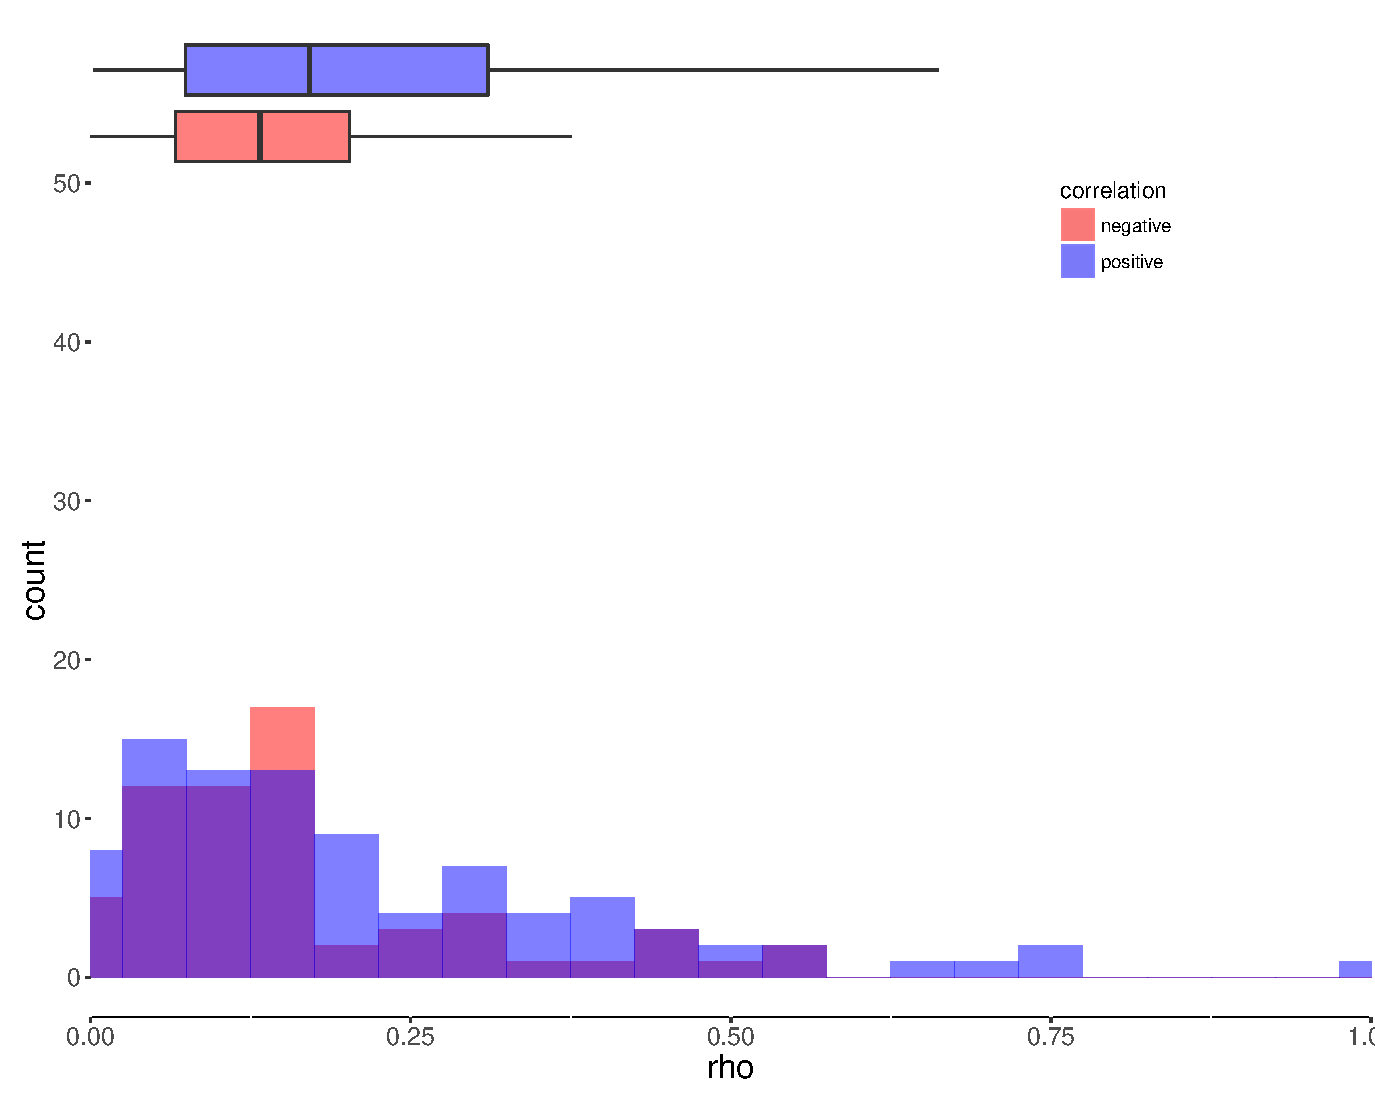
\includegraphics[width = 1\textwidth]{figures/combinedplotWJ_ws.pdf}
        \caption{.s.}
        \label{fig:.}
    \end{subfigure}
\caption{.}
    \label{fig:.}
\end{figure}

Dry season network (Figure \ref{fig:networkCP_ds}) is comprised of 18 associated injuries and  60 associations (edges). The network show two groups of injury syndromes (the combination of injuries) based on the optimal clustering algorithm. Group1 (green) was more closely clustered than another group, according to node properties. The injuries in group1 (WH, SHR, SHB, DP, BS, RH, NB, DH, FS, HB, and RS) have high clustering coefficient This indicate that these injuries form complex co-occurrence relationships. Network properties (Figure \ref{fig:nodepropCP_ds}) reveal WM and LF, BS, BLB, NBS are high-betweenness nodes. As opposed to other injuries, LB and BLS had low scores on at least two centrality measures. Apparently, LB occur less possibly (low betweenness), and did not occur with other injuries (low degree and clustering coefficient). Because of high value of centrality, WM and BS can be indicators for monitoring the injury occurrence in each syndrome.

In wet season, the co-occurrence network of rice injuries (Figure \ref{fig:networkCP_ws}) reveals 4 syndromes, 20 injuries, and 48 significant relationships (edges). Syndrome3 (purple) is comprised of BLS, RS, HB, SHB, SHR and WM. They were placed closer to each other than other syndromes based on the structure and clustering coefficient (Figure \ref{fig:nodepropCP_ws}). This syndrome also links with syndrome1, 2 and 4. Based on network structure and betweenness, WM can be an indicator for monitoring pest and disease incidence in this season, and it also is the injury in syndrome3, which is the central syndrome of this network. 

\begin{figure}
    \centering
    \begin{subfigure}[b]{1\textwidth}
        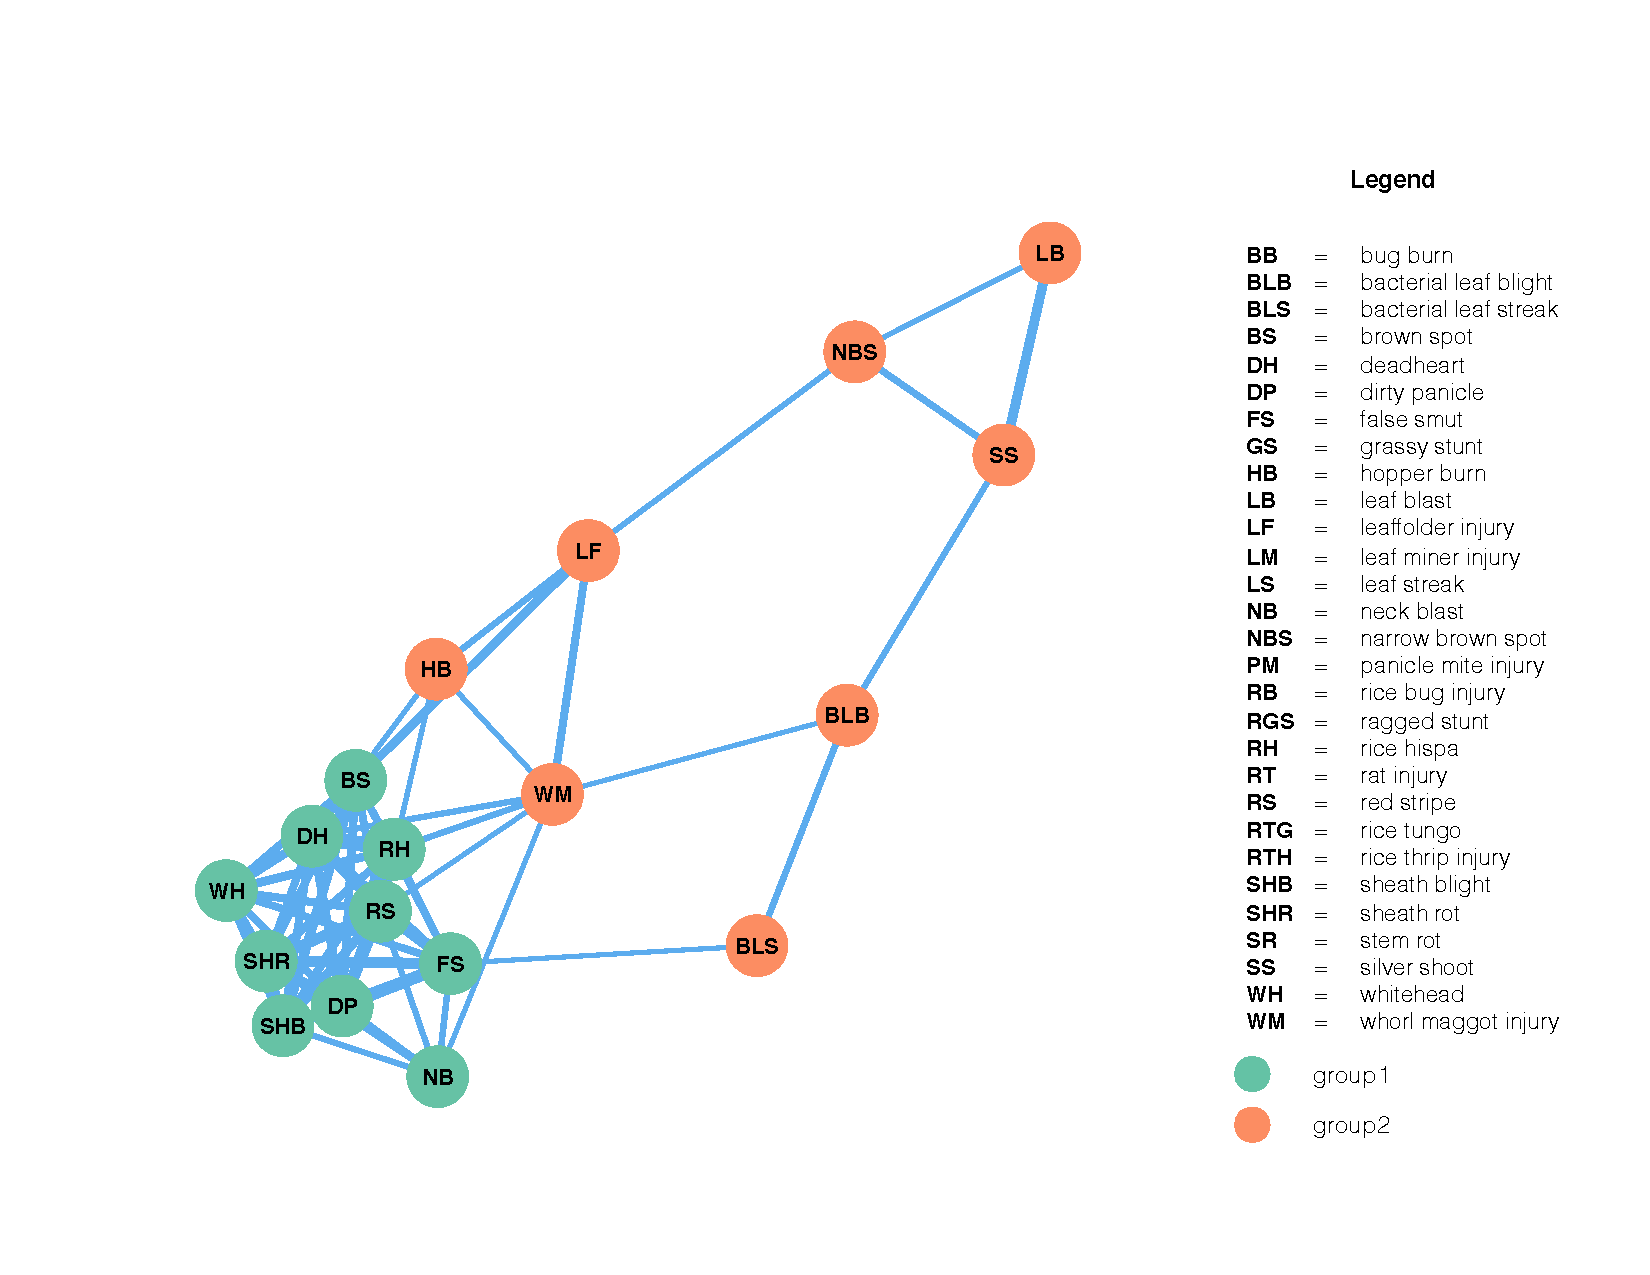
\includegraphics[width = 1\textwidth]{figures/networkCP_ds/networkCP_ds.pdf}
        \caption{Co-occurrence network of rice injuries in dry season at Central Plain, Thailand. The layout of the network graph is based on the Fruchterman-Reingold algorithm, which places nodes with stronger or more connections closer to each other.}
        \label{fig:networkCP_ds}
    \end{subfigure}
    \begin{subfigure}[b]{1\textwidth}
        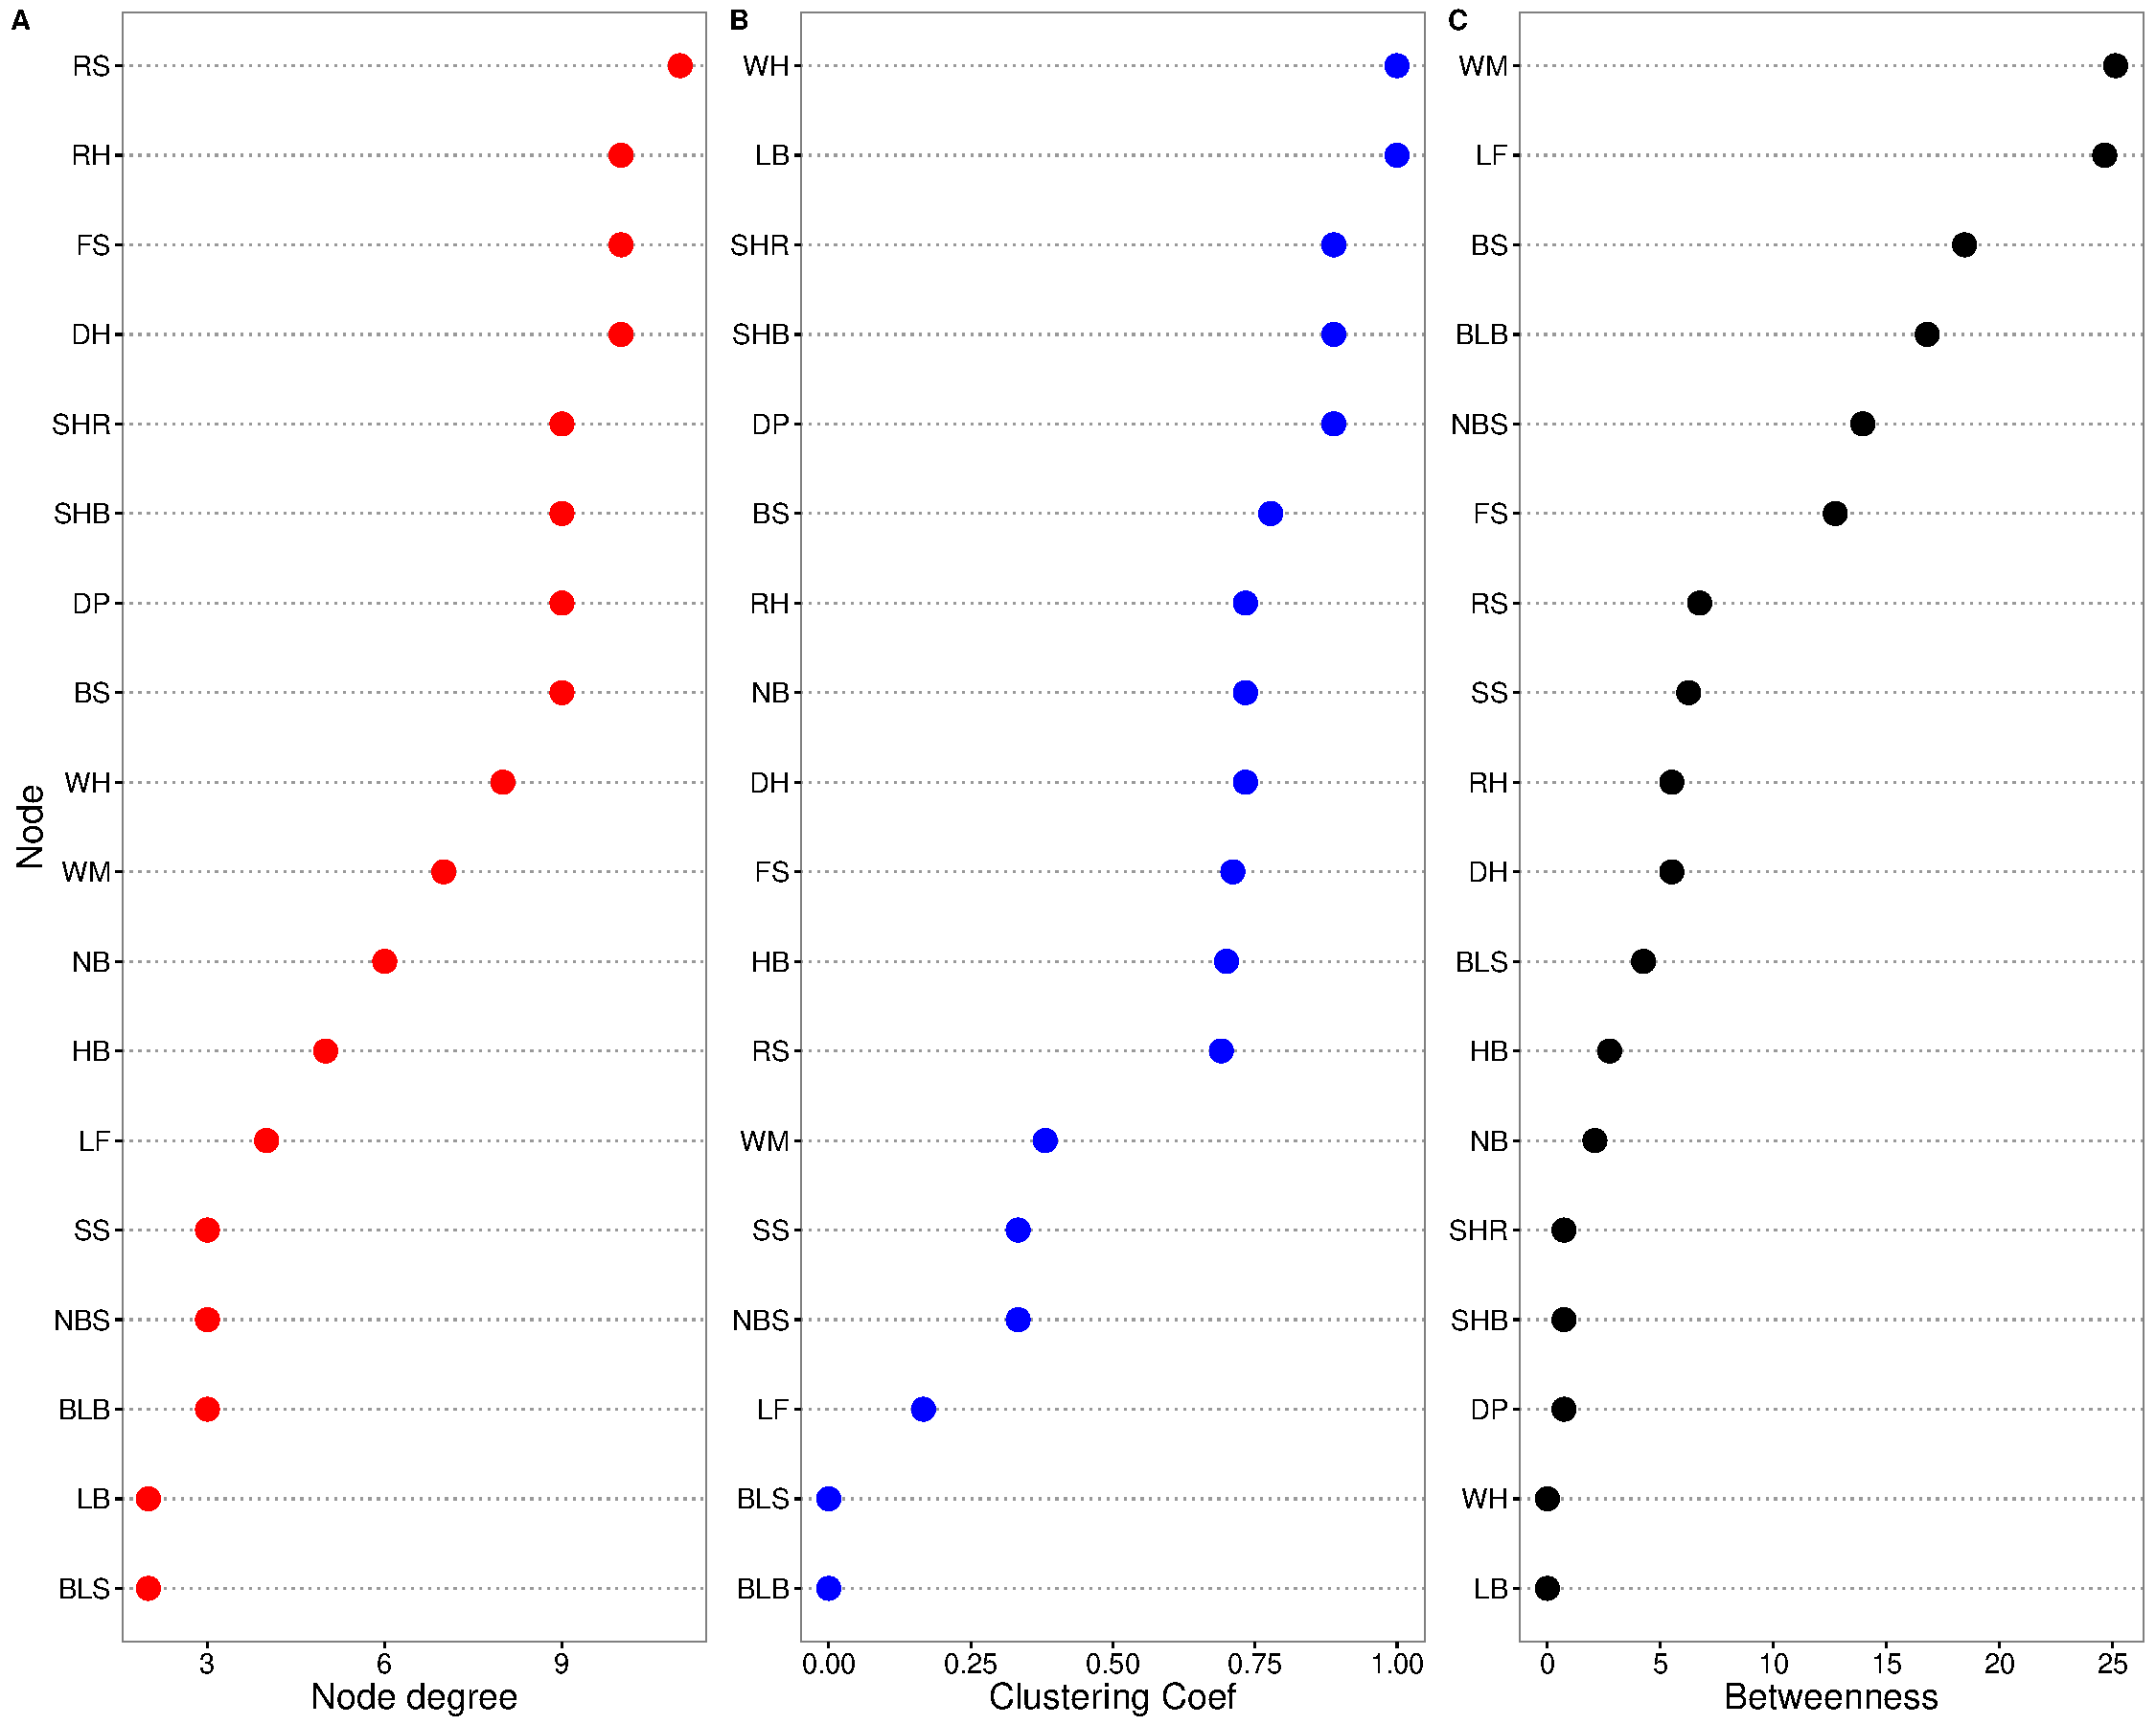
\includegraphics[width = 1\textwidth]{figures/nodepropCP_ds/nodepropCP_ds.pdf}
        \caption{Three centrality measures of the nodes in co-occurrence network of rice injuries in dry season at Central Plain. A: node degree, B:clustering coefficient, and C:Betweenness.}
        \label{fig:nodepropCP_ds}
    \end{subfigure}
    \caption{Network analysis of rice injury co-occurrence in wet season at Central Plain, Thailand}
    \label{fig:CP_ds}
\end{figure}

\begin{figure}
    \centering
    \begin{subfigure}[b]{1\textwidth}
        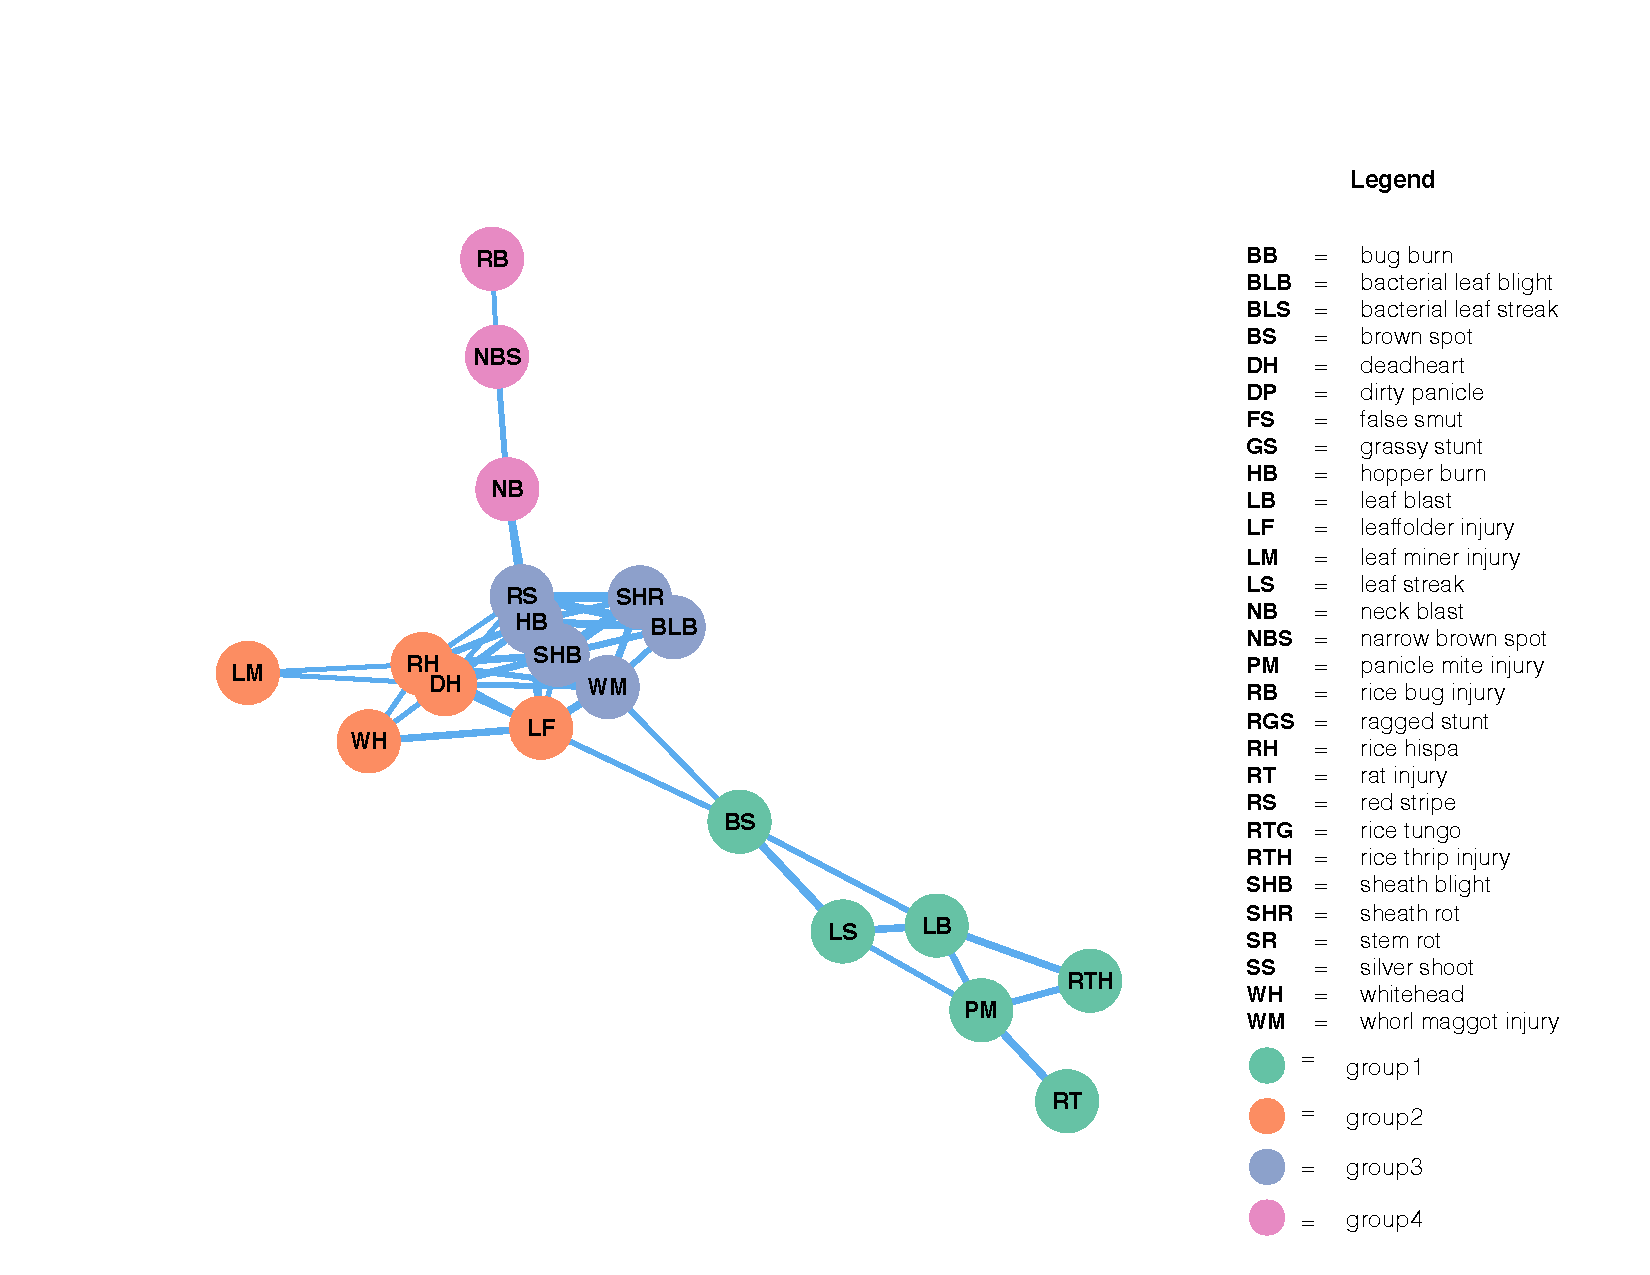
\includegraphics[width = 1\textwidth]{figures/networkCP_ws/networkCP_ws.pdf}
        \caption{Co-occurrence network of rice injuries in dry season at Central Plain, Thailand. The layout of the network graph is based on the Fruchterman-Reingold algorithm, which places nodes with stronger or more connections closer to each other.}
        \label{fig:networkCP_ws}
    \end{subfigure}
    \begin{subfigure}[b]{1\textwidth}
        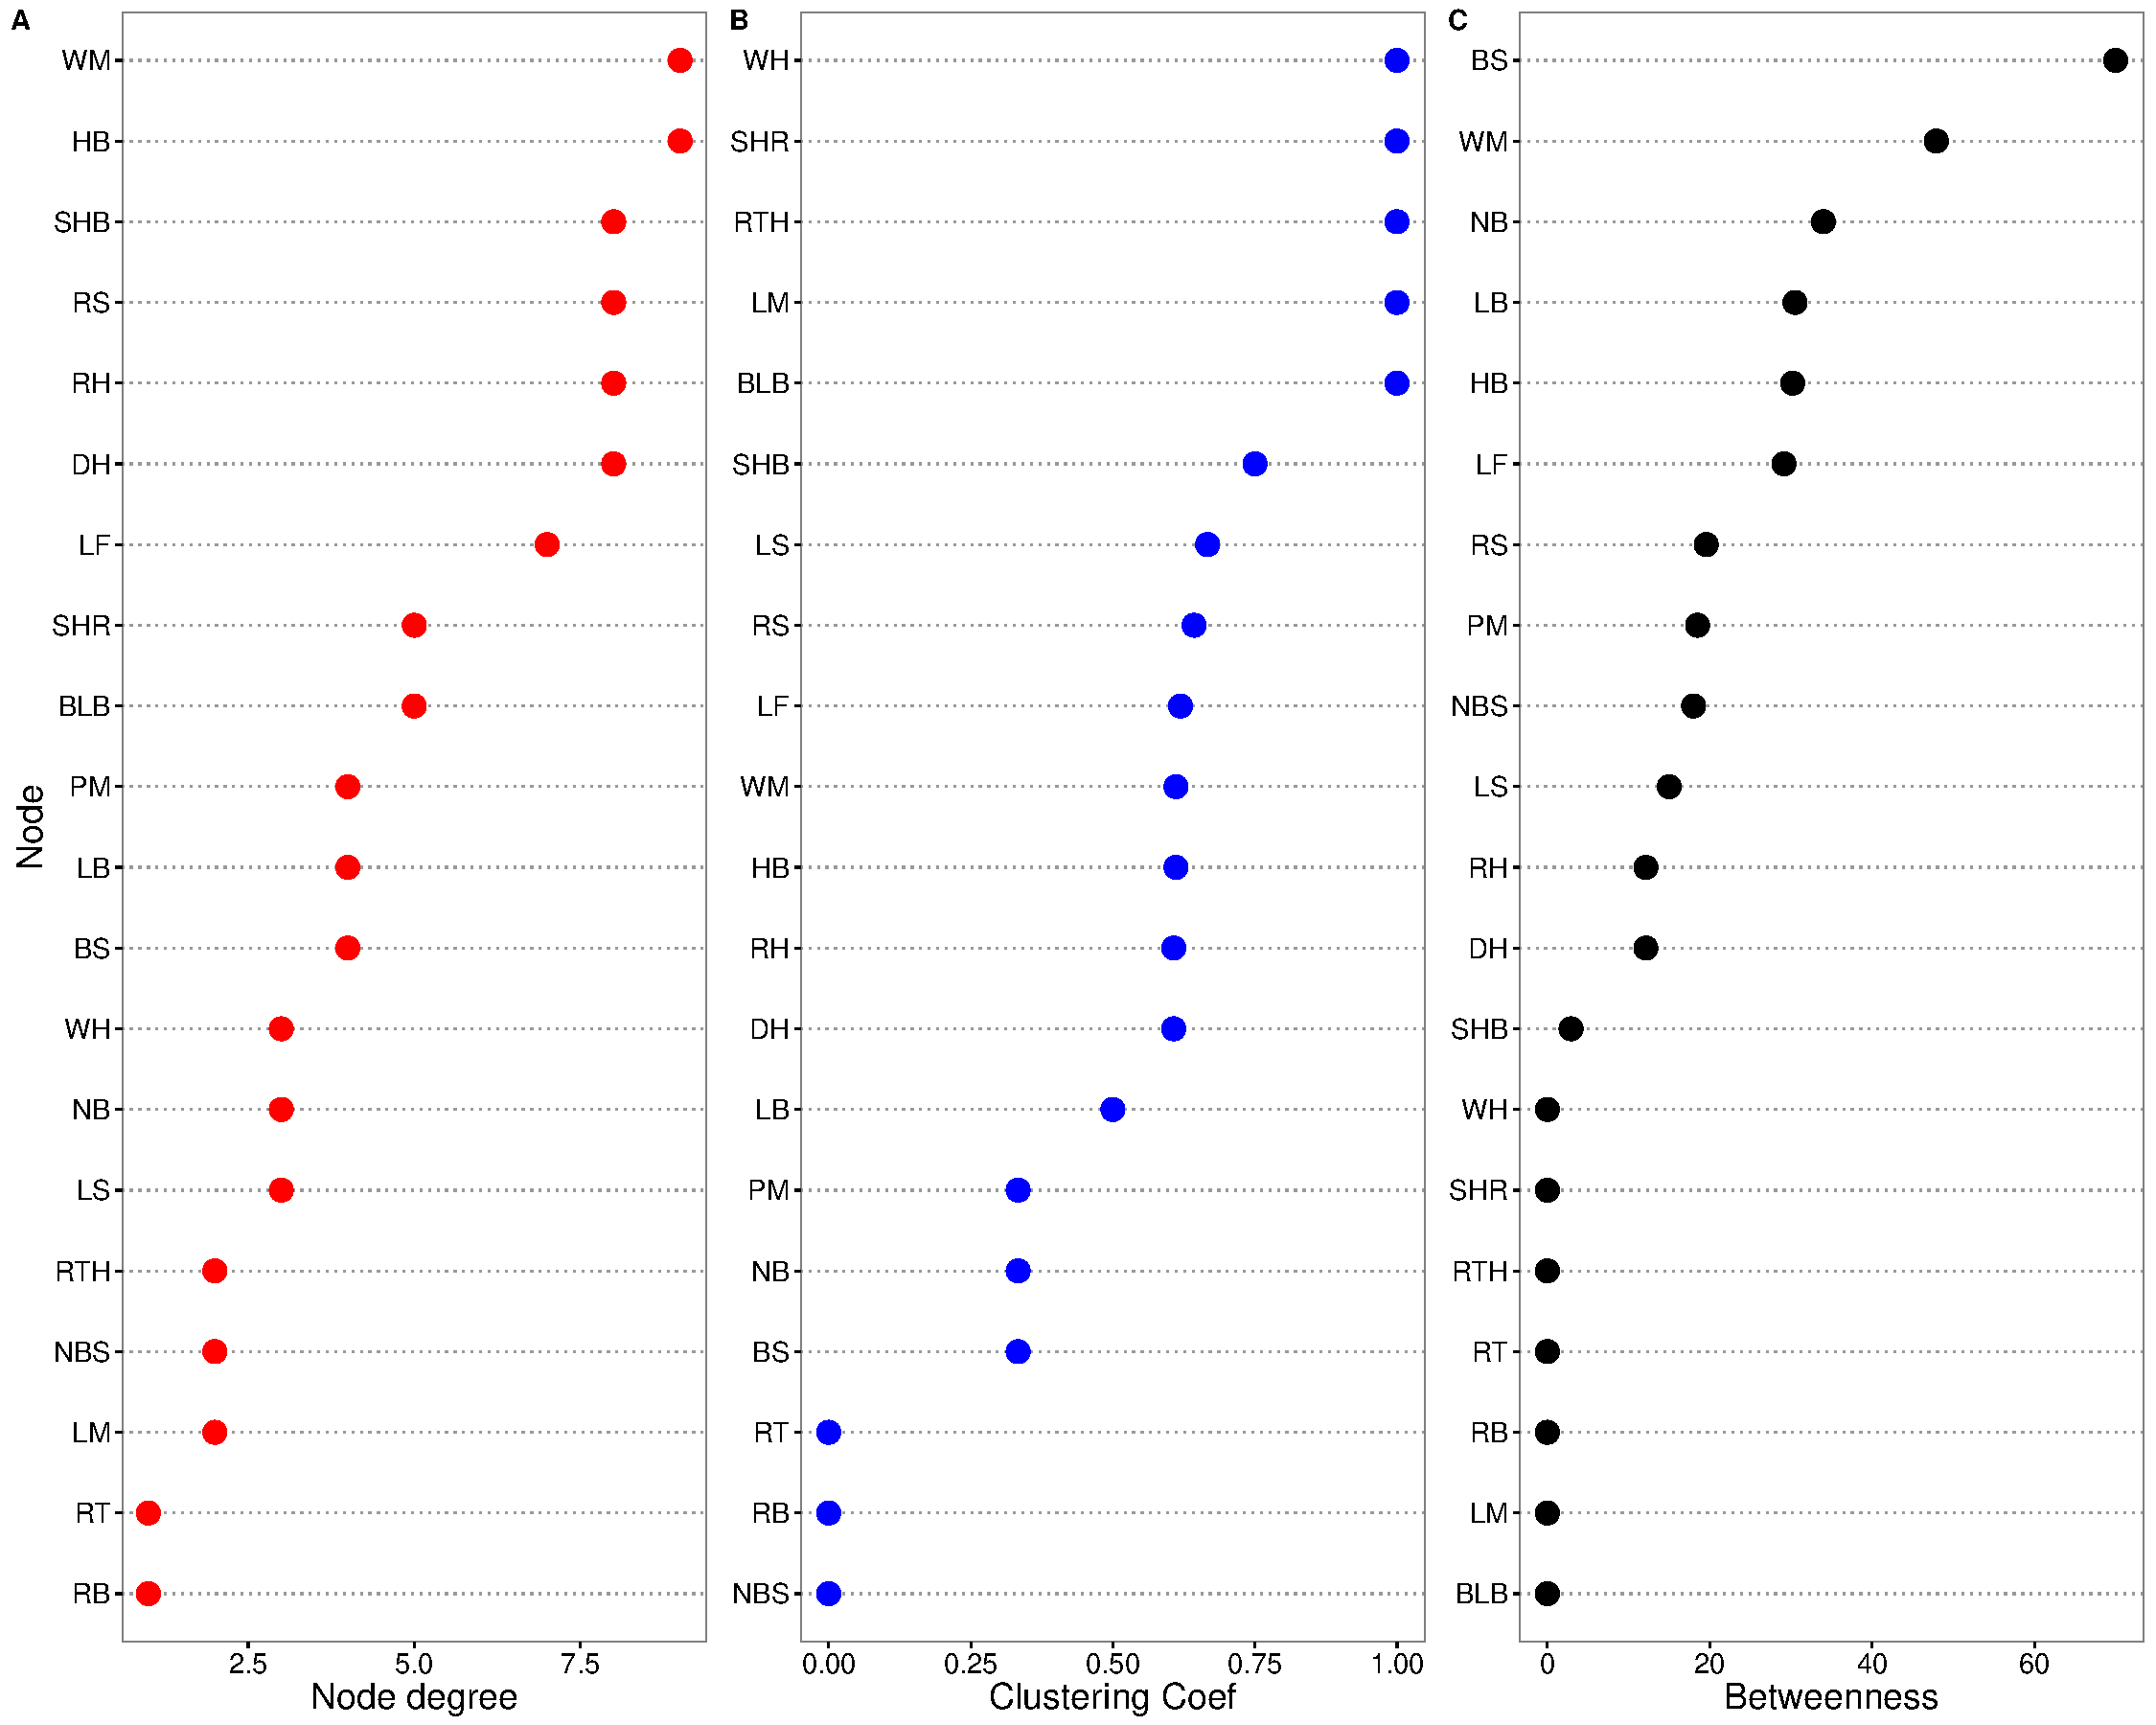
\includegraphics[width = 1\textwidth]{figures/nodepropCP_ws/nodepropCP_ws.pdf}
        \caption{Three centrality measures of the nodes in co-occurrence network of rice injuries in dry season at Central Plain. A: node degree, B:clustering coefficient, and C:Betweenness}
        \label{fig:nodepropCP_ws}
    \end{subfigure}
    \caption{Network analysis of rice injury co-occurrence in wet season at Central Plain, Thailand}
    \label{fig:CP_ws}
\end{figure}

\textbf{Odisha, India}

Co-occurrence network of rice injuries in dry season (Figure \ref{fig:networkOR_ds}) consists of of 9 associated injuries and 13 associations. The network shows two isolated injury syndromes. One was the combination of BS, BLB, WM and SHB. Another was RH, WH, DH, LB, NB. This network suggests indicators for monitoring such as LB for syndrome1, and WM, SHB, BS, and BLB for syndrome2 base on centrality (Figure \ref{fig:nodepropOR_ds}).  

The network in wet season (Figure \ref{fig:networkOR_ws}) is more complex than the network in dry season. It is comprised of 15 nodes with 26 edges. The network reveals four syndromes. Syndrome4, composed of LB, LM and WM, is isolated from the rest. Syndrome2 is placed in between syndrome1 and 3. The injuries in syndrome2 have high value of node degree and clustering coefficient (Figure \ref{fig:nodepropOR_ws}), which mean they were connected to many injuries. NBS and LF, injuries in group1 and group2, respectively present high betweenness values and connected to injuries of group3. They are also good indicators for monitoring. This indicated that injuries of syndrome3 have high chance to occur together with group1 and 2, but not group4. 

\begin{figure}
    \centering
    \begin{subfigure}[b]{1\textwidth}
        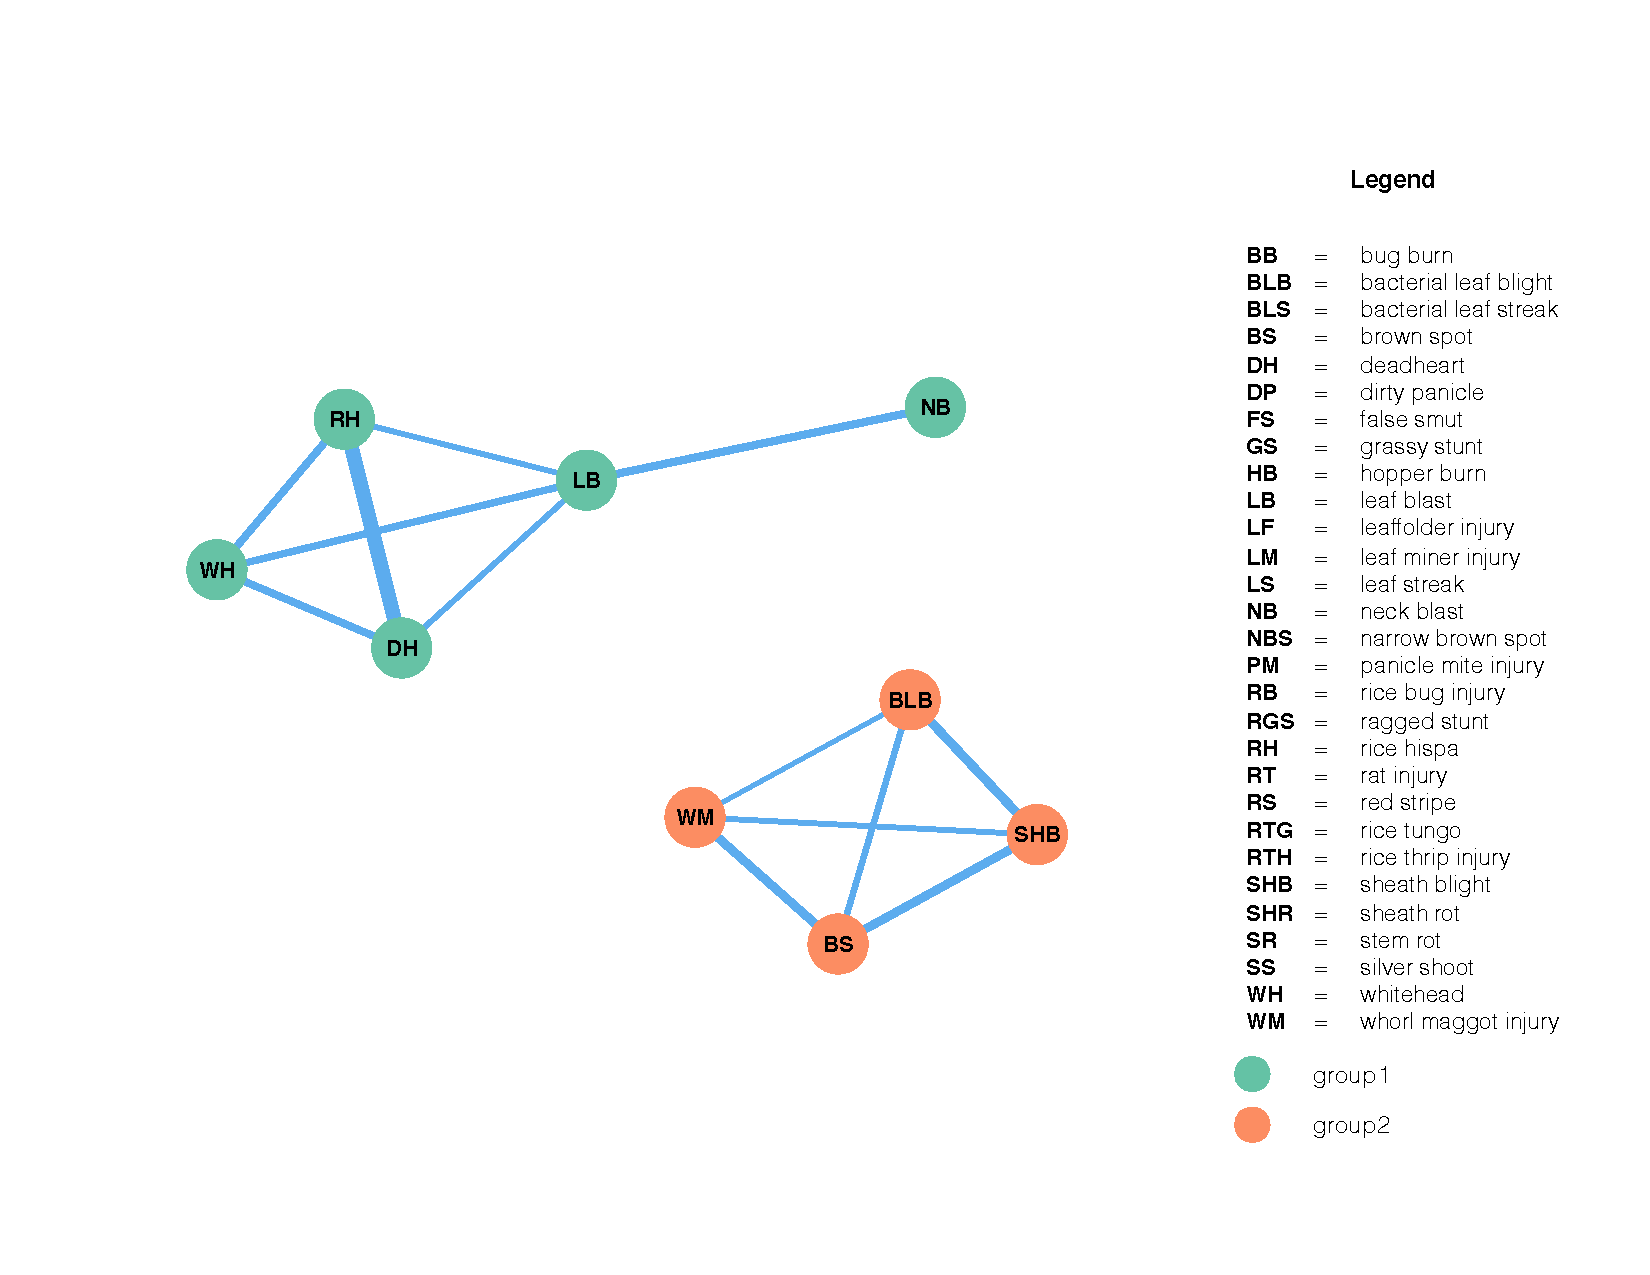
\includegraphics[width = 1\textwidth]{figures/networkOR_ds/networkOR_ds.pdf}
        \caption{Co-occurrence network of rice injuries in wet season at Odisha, India. The layout of the network graph is based on the Fruchterman-Reingold algorithm, which places nodes with stronger or more connections closer to each other.}
        \label{fig:networkOR_ds}
    \end{subfigure}
    \begin{subfigure}[b]{1\textwidth}
        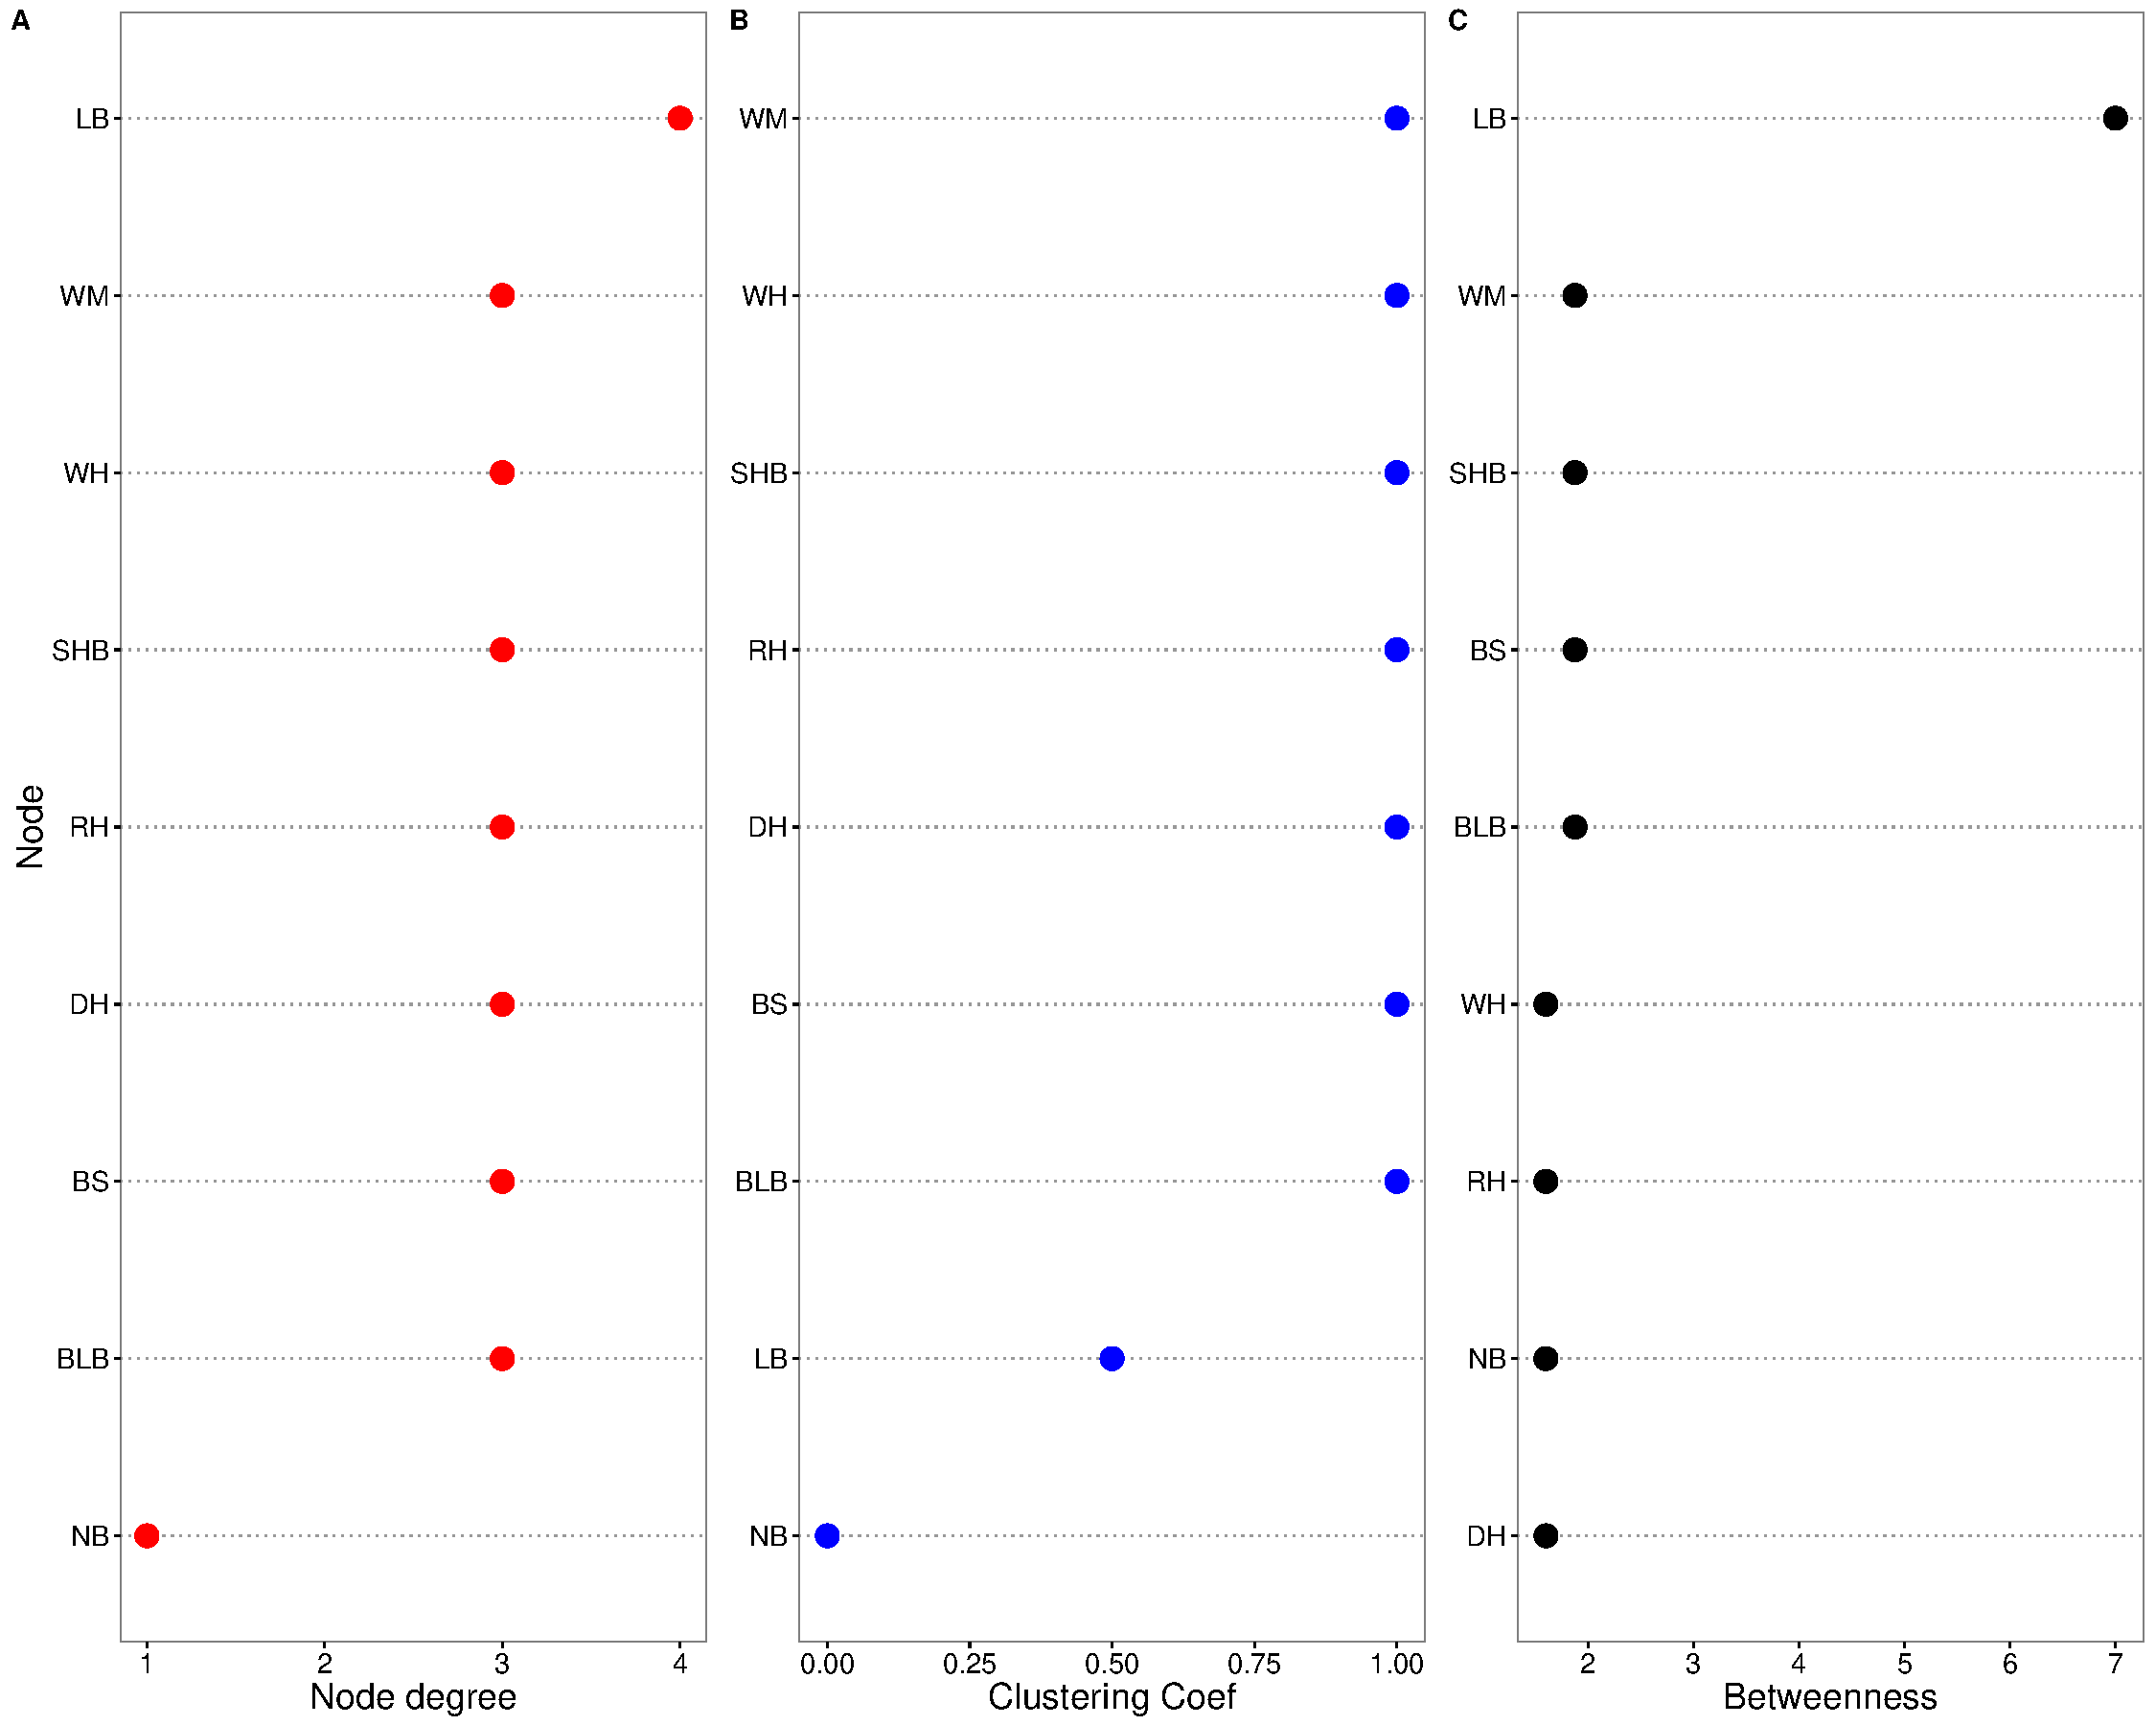
\includegraphics[width = 1\textwidth]{figures/nodepropOR_ds/nodepropOR_ds.pdf}
        \caption{Three centrality measures of the nodes in co-occurrence network of rice injuries in dry season at Odisha, India. A: node degree, B:clustering coefficient, and C:Betweenness.}
        \label{fig:nodepropOR_ds}
    \end{subfigure}
    \caption{Network analysis of rice injury co-occurrence in dry season at Odisha, India}
    \label{fig:OR_ds}
\end{figure}

\begin{figure}
    \centering
    \begin{subfigure}[b]{1\textwidth}
        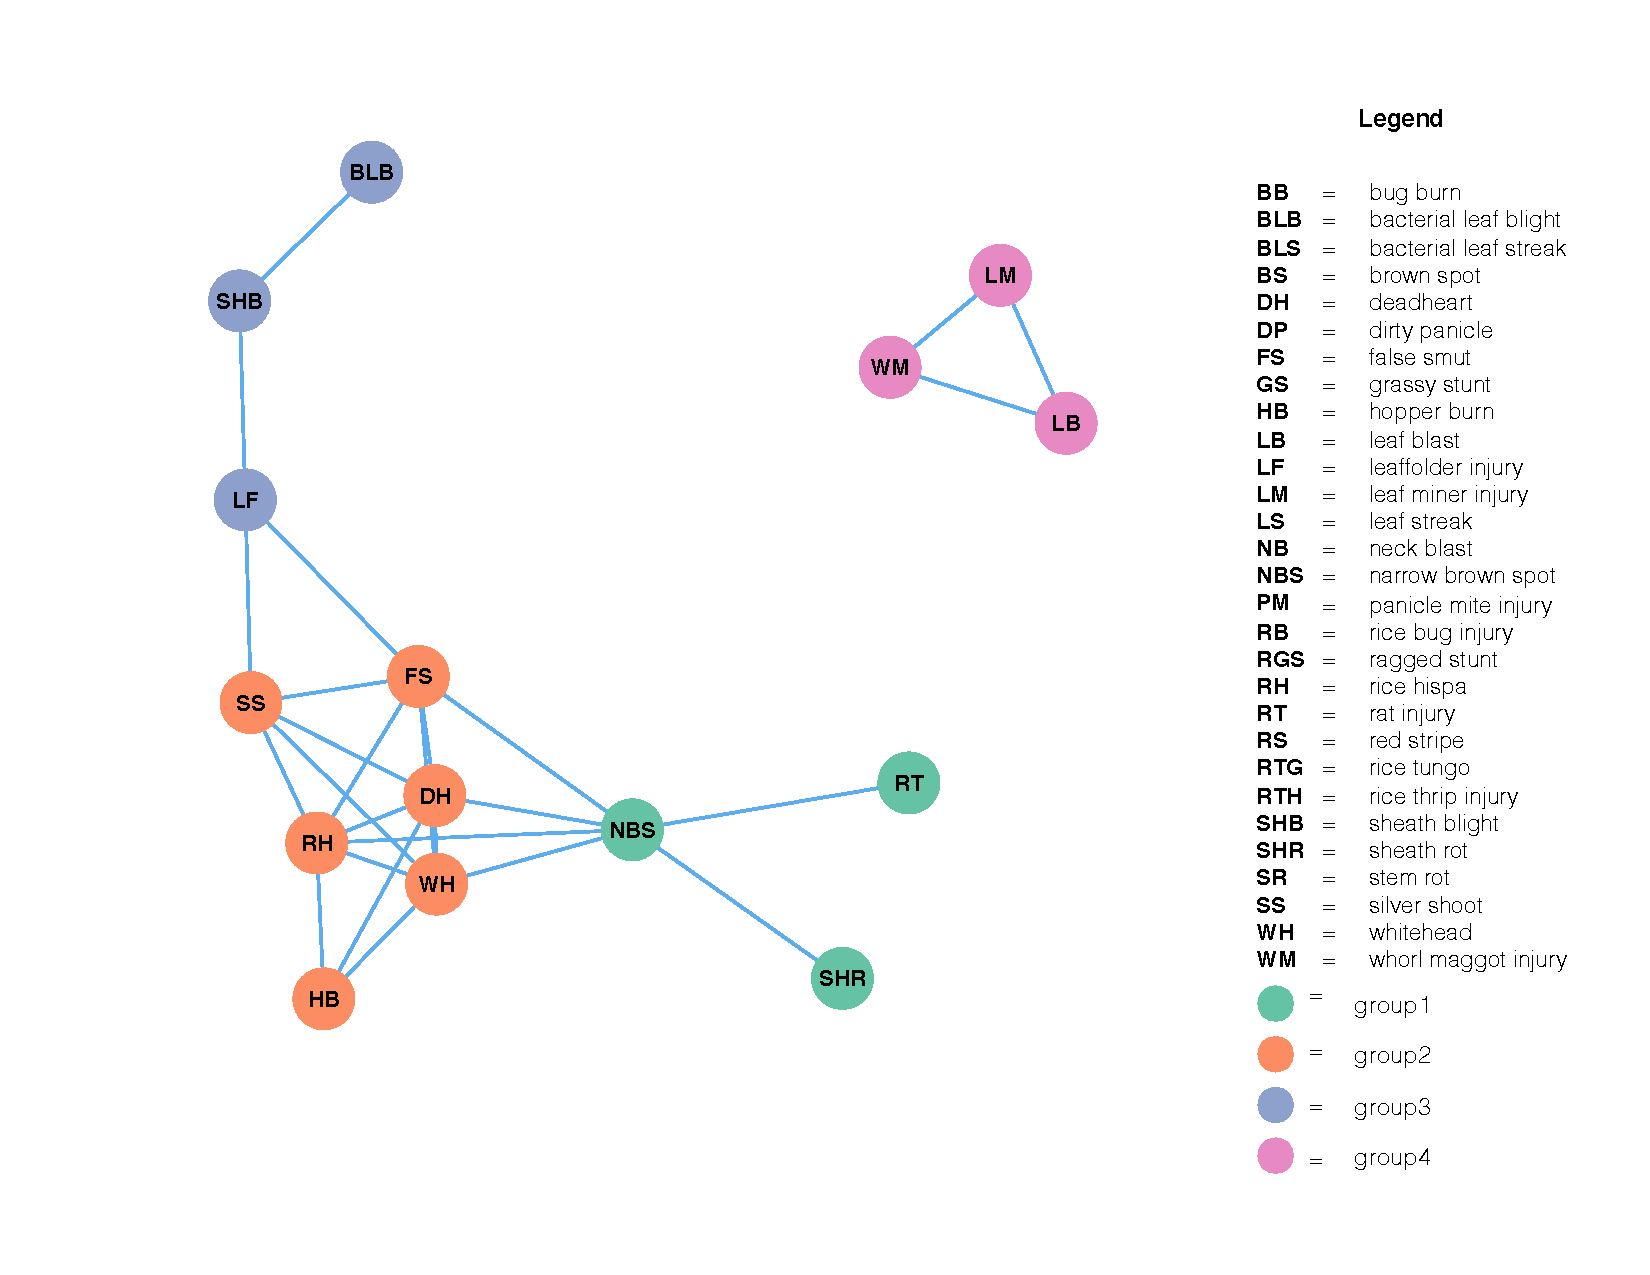
\includegraphics[width = 1\textwidth]{figures/networkOR_ws/networkOR_ws.pdf}
        \caption{Co-occurrence network of rice injuries in wet season at Odisha, India. The layout of the network graph is based on the Fruchterman-Reingold algorithm, which places nodes with stronger or more connections closer to each other.}
        \label{fig:networkOR_ws}
    \end{subfigure}
    \begin{subfigure}[b]{1\textwidth}
        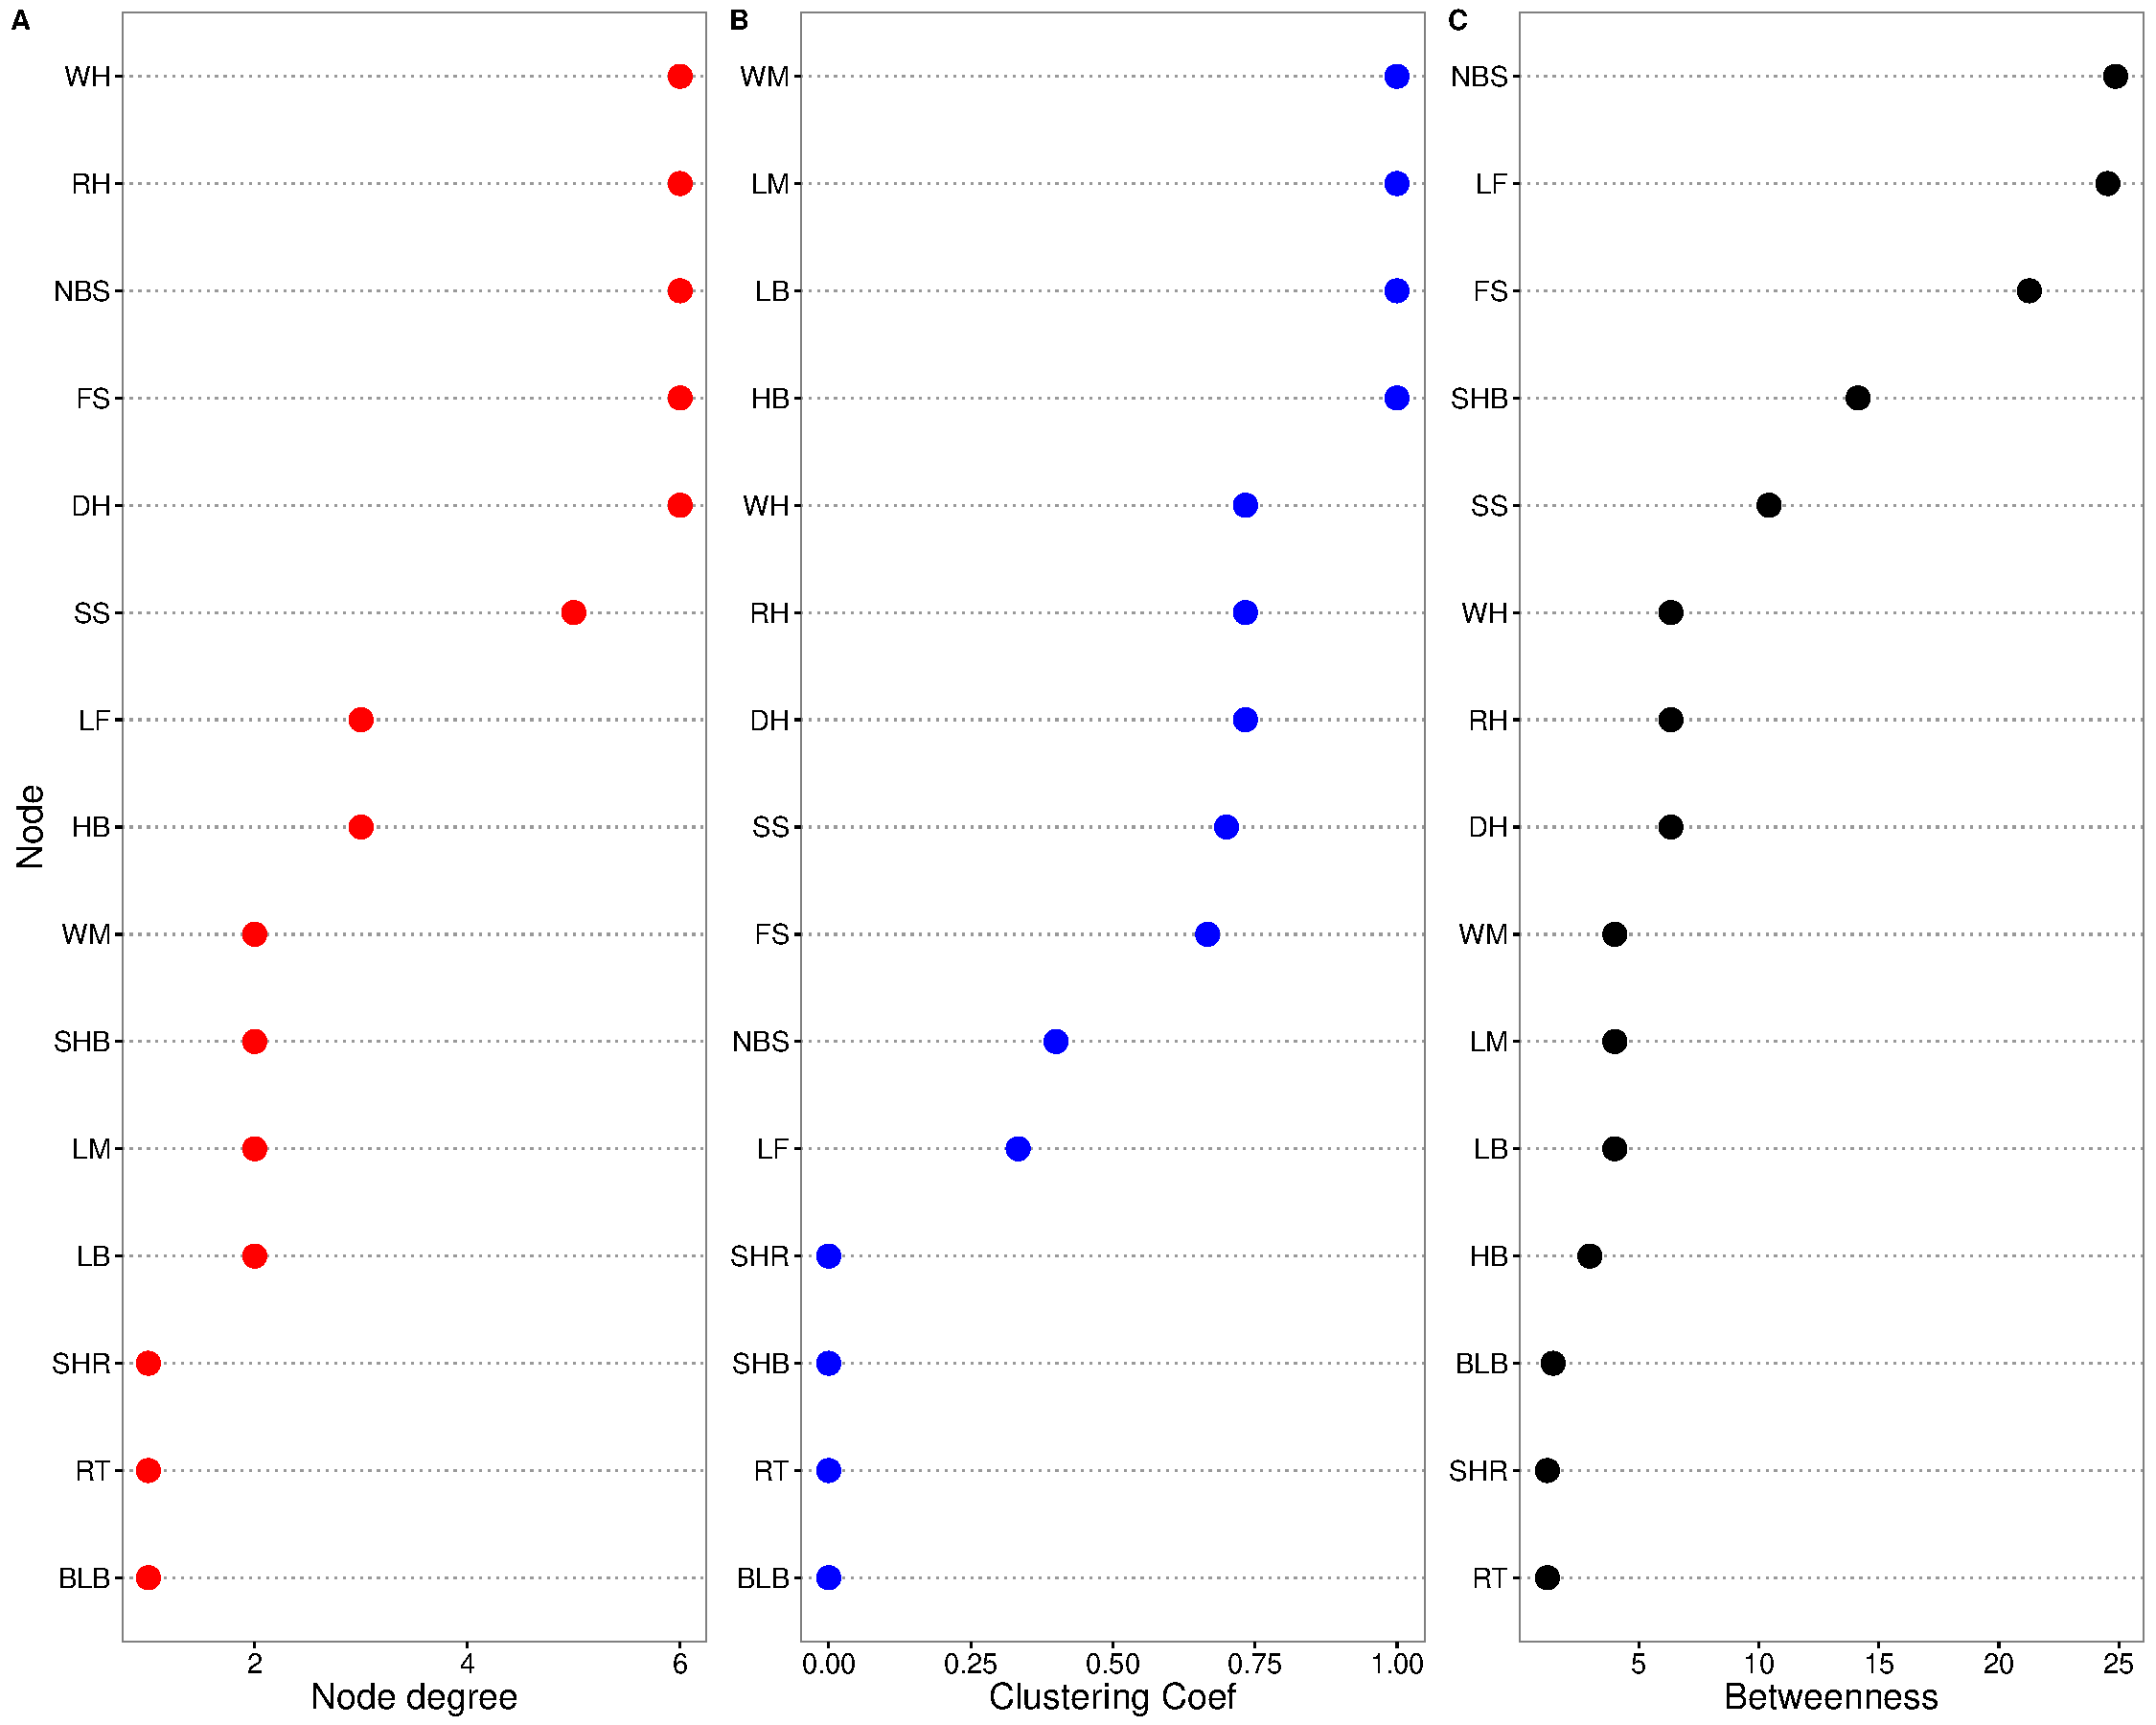
\includegraphics[width = 1\textwidth]{figures/nodepropOR_ws/nodepropOR_ws.pdf}
        \caption{Three centrality measures of the nodes in co-occurrence network of rice injuries in wet season at Odisha, India. A: node degree, B:clustering coefficient, and C:Betweenness.}
        \label{fig:nodepropOR_ws}
    \end{subfigure}
    \caption{Network analysis of rice injury co-occurrence in wet season at Odisha, India}
    \label{fig:OD_ws}
\end{figure}


\textbf{Red River Delta, Vietnam}
 
Co-occurrence network of rice injuries in dry season (Fig. \ref{fig:networkRR_ds}) is comprised of 19 nodes and 26 associations. The network reveals three isolated syndromes, and two connected syndromes. BB of syndrome1 and SHB of syndrome3 can be indicators because of high values of centrality measures (Figure \ref{fig:nodepropRR_ds}).

Wet season network (Figure \ref{fig:networkRR_ws})) consists of 18 injuries with 37 associations. It reveals 4 connected syndromes and an isolated syndrome. Group2 was located that could connect to Group3, 4, 5. According to Figure \ref{fig:nodepropRR_ws}, BLB, DP could be good indicator, because they are likely to occur (high betweenness) and when they occurred, other injuries in other syndromes, except syndrome5 (high node degree) could be possibly observed. 


\begin{figure}
    \centering
    \begin{subfigure}[b]{1\textwidth}
        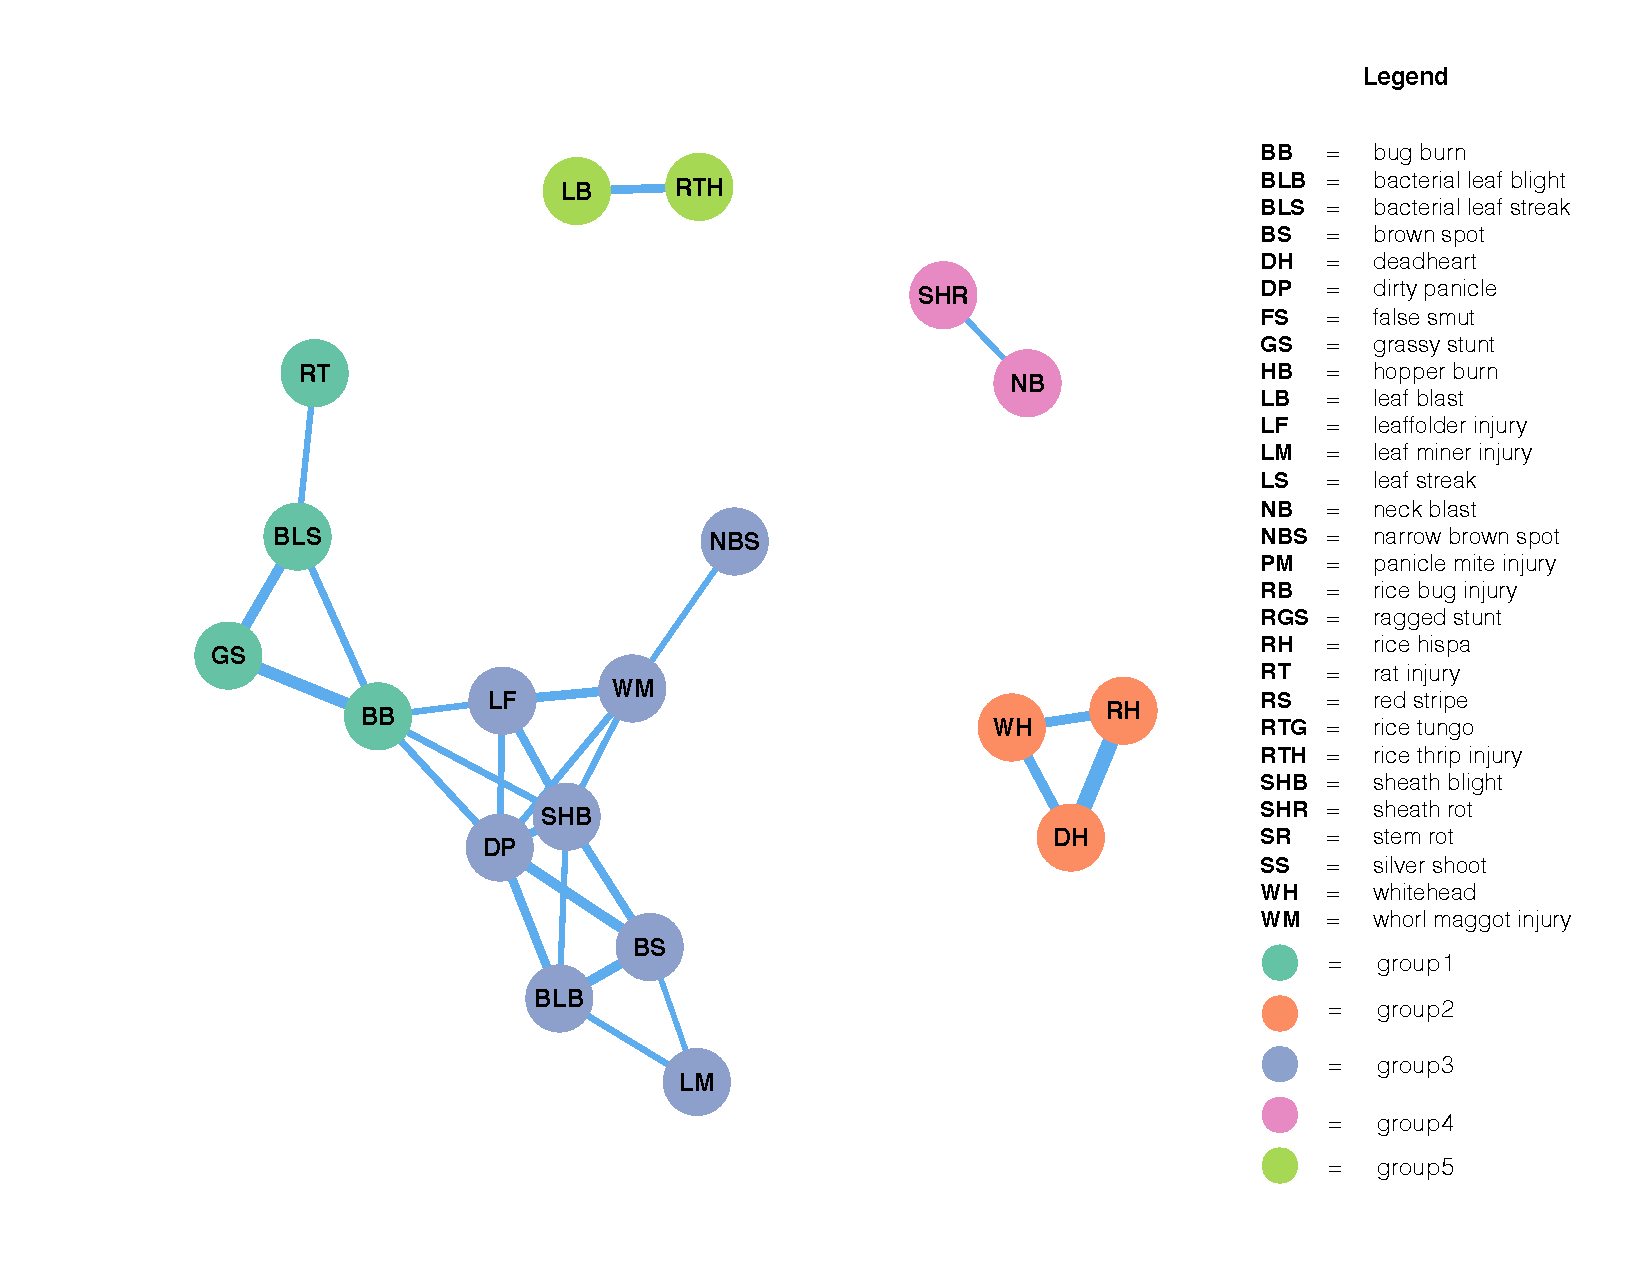
\includegraphics[width = 1\textwidth]{figures/networkRR_ds/networkRR_ds.pdf}
        \caption{Co-occurrence network of rice injuries in dry season at Red River Delta, Vietnam. The layout of the network graph is based on the Fruchterman-Reingold algorithm, which places nodes with stronger or more connections closer to each other.}
        \label{fig:networkRR_ds}
    \end{subfigure}
    \begin{subfigure}[b]{1\textwidth}
        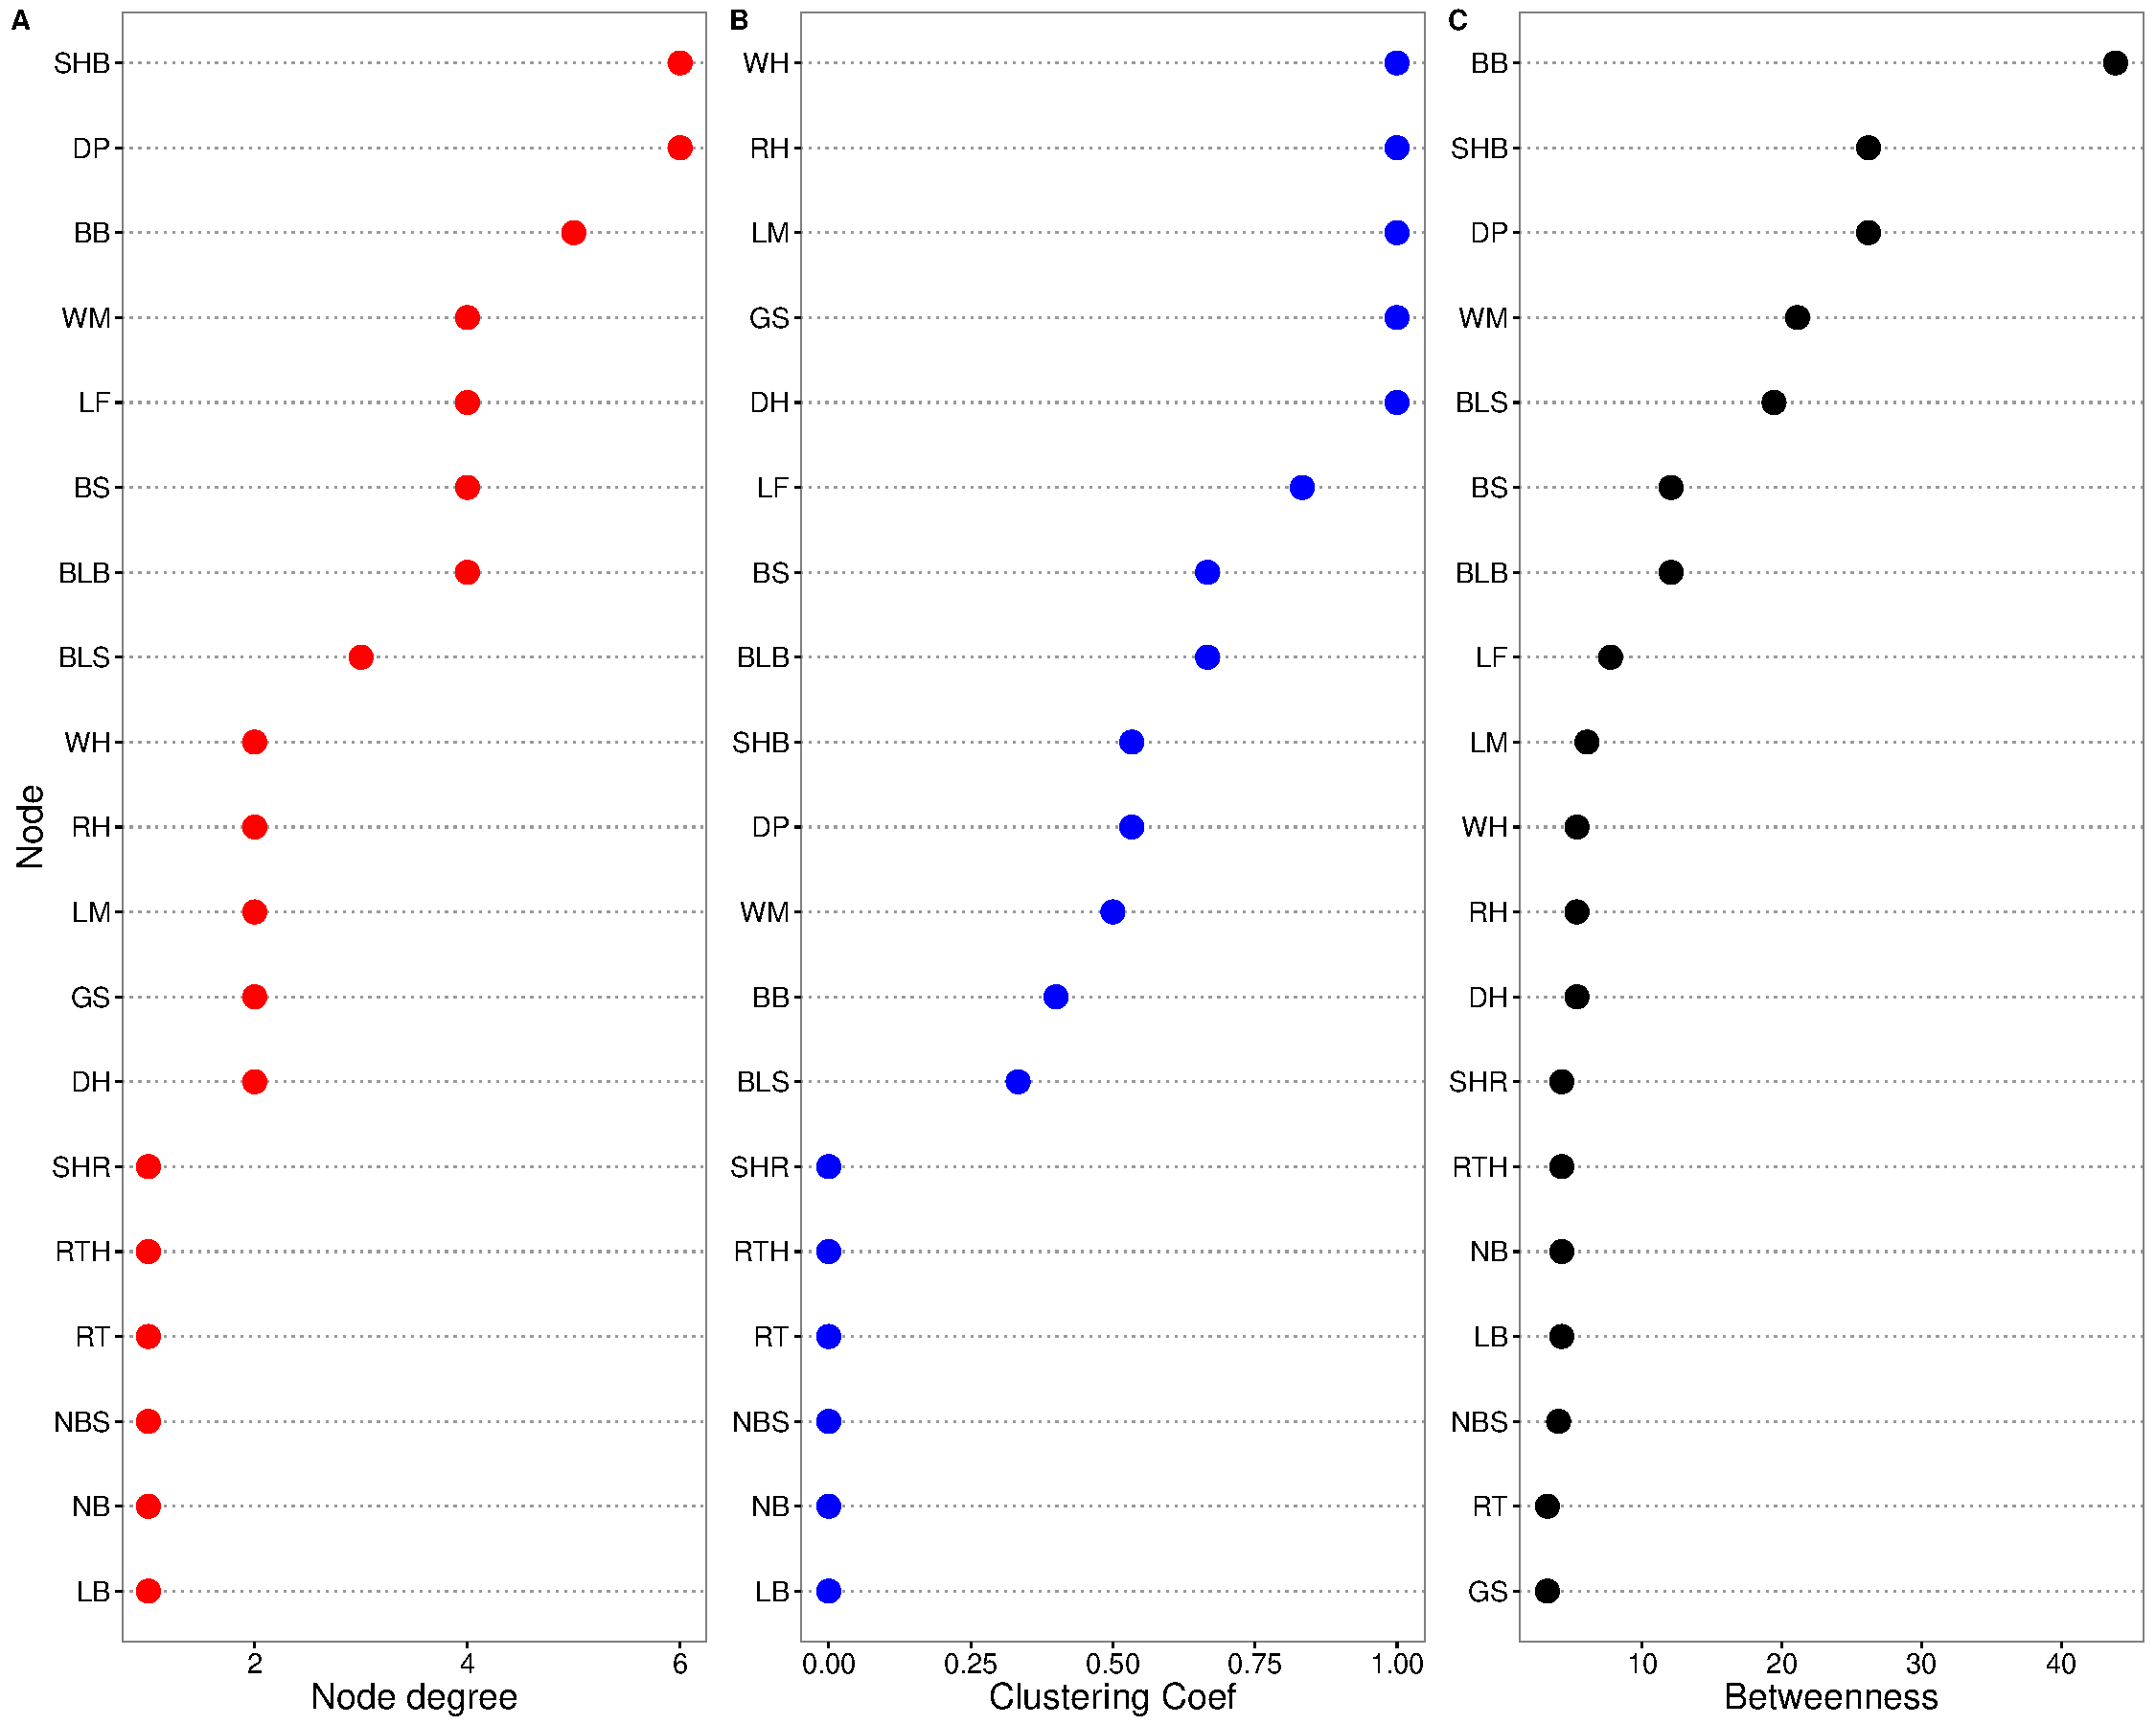
\includegraphics[width = 1\textwidth]{figures/nodepropRR_ds/nodepropRR_ds.pdf}
        \caption{Three centrality measures of the nodes in co-occurrence network of rice injuries in dry season at Red River Delta, Vietnam. A: node degree, B:clustering coefficient, and C:Betweenness}
        \label{fig:nodepropRR_ds}
    \end{subfigure}
    \caption{Network analysis of rice injury co-occurrence in dry season at Red River Delta, Vietnam}
    \label{fig:RR_ds}
\end{figure}

\begin{figure}
    \centering
    \begin{subfigure}[b]{1\textwidth}
        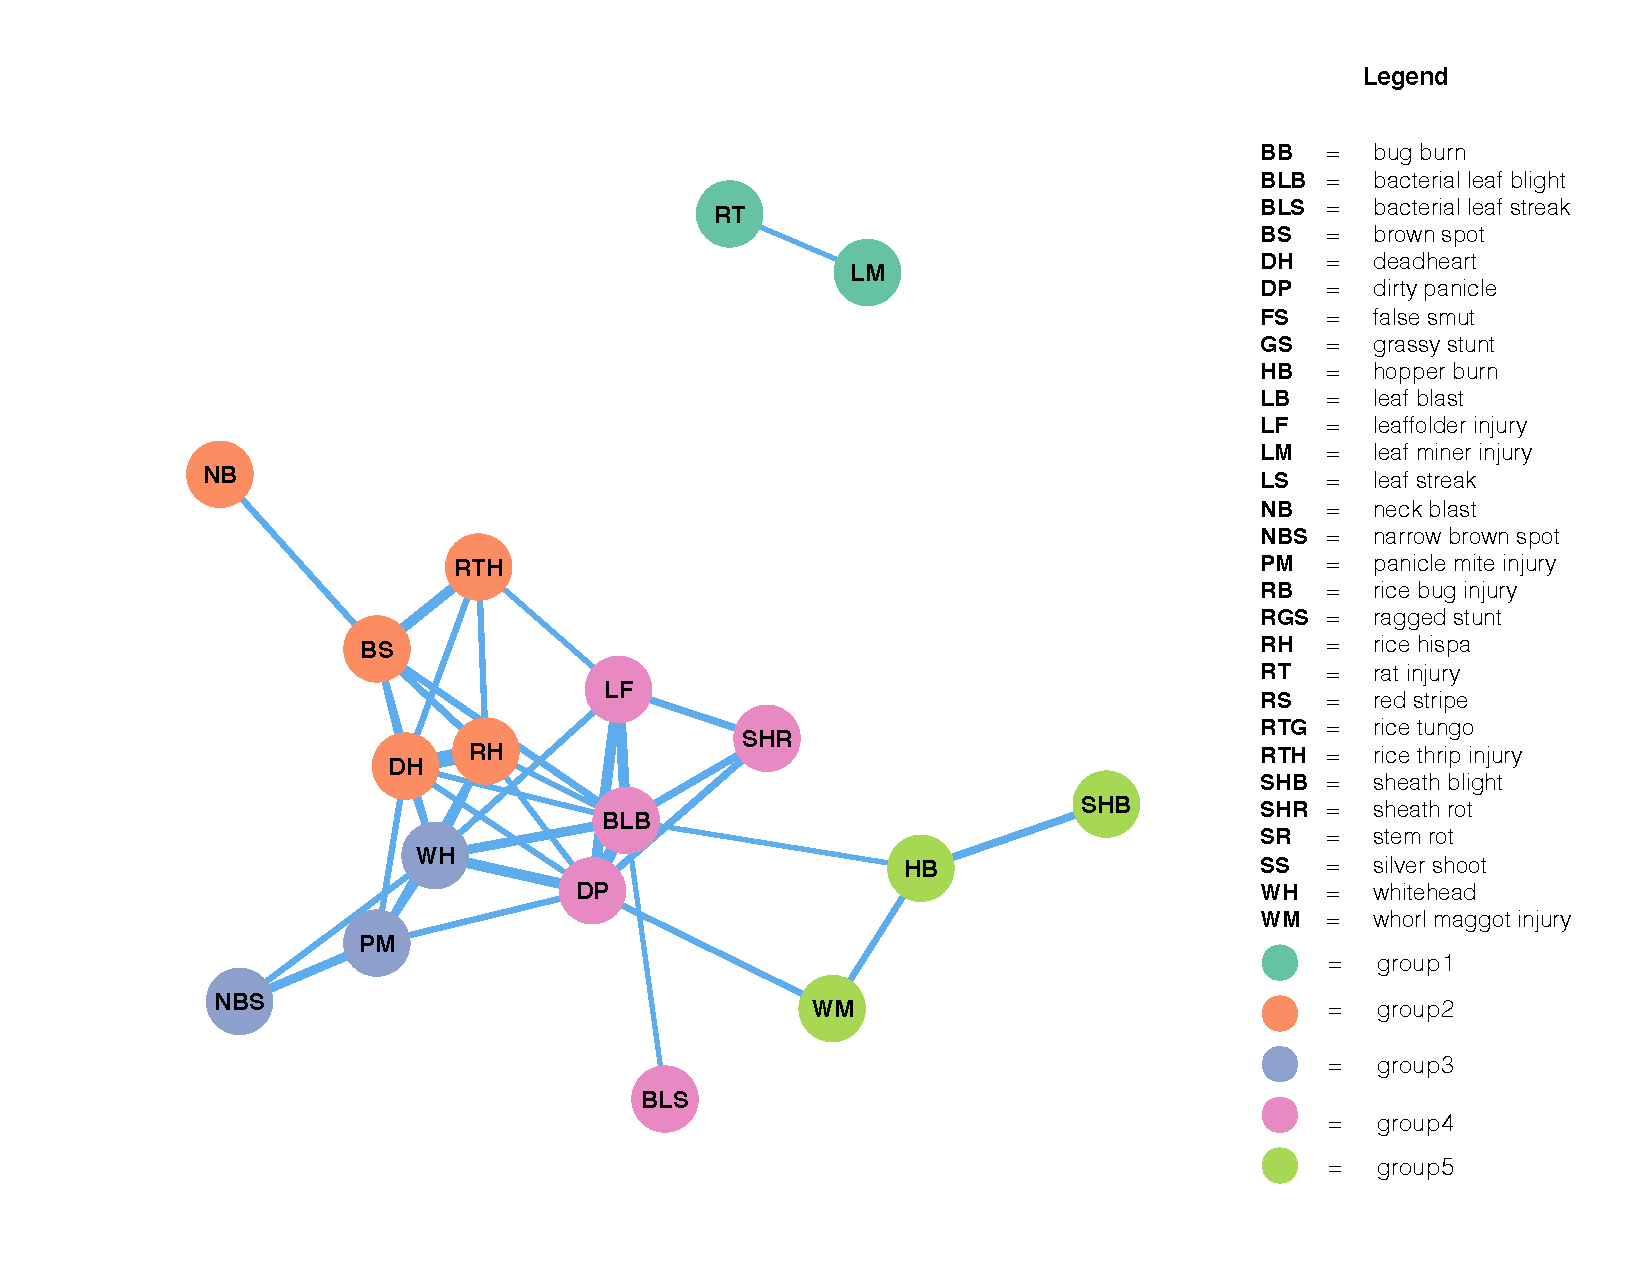
\includegraphics[width = 1\textwidth]{figures/networkRR_ws/networkRR_ws.pdf}
        \caption{Co-occurrence network of rice injuries in wet season at Red River Delta, Vietnam. The layout of the network graph is based on the Fruchterman-Reingold algorithm, which places nodes with stronger or more connections closer to each other.}
        \label{fig:networkRR_ws}
    \end{subfigure}
    \begin{subfigure}[b]{1\textwidth}
        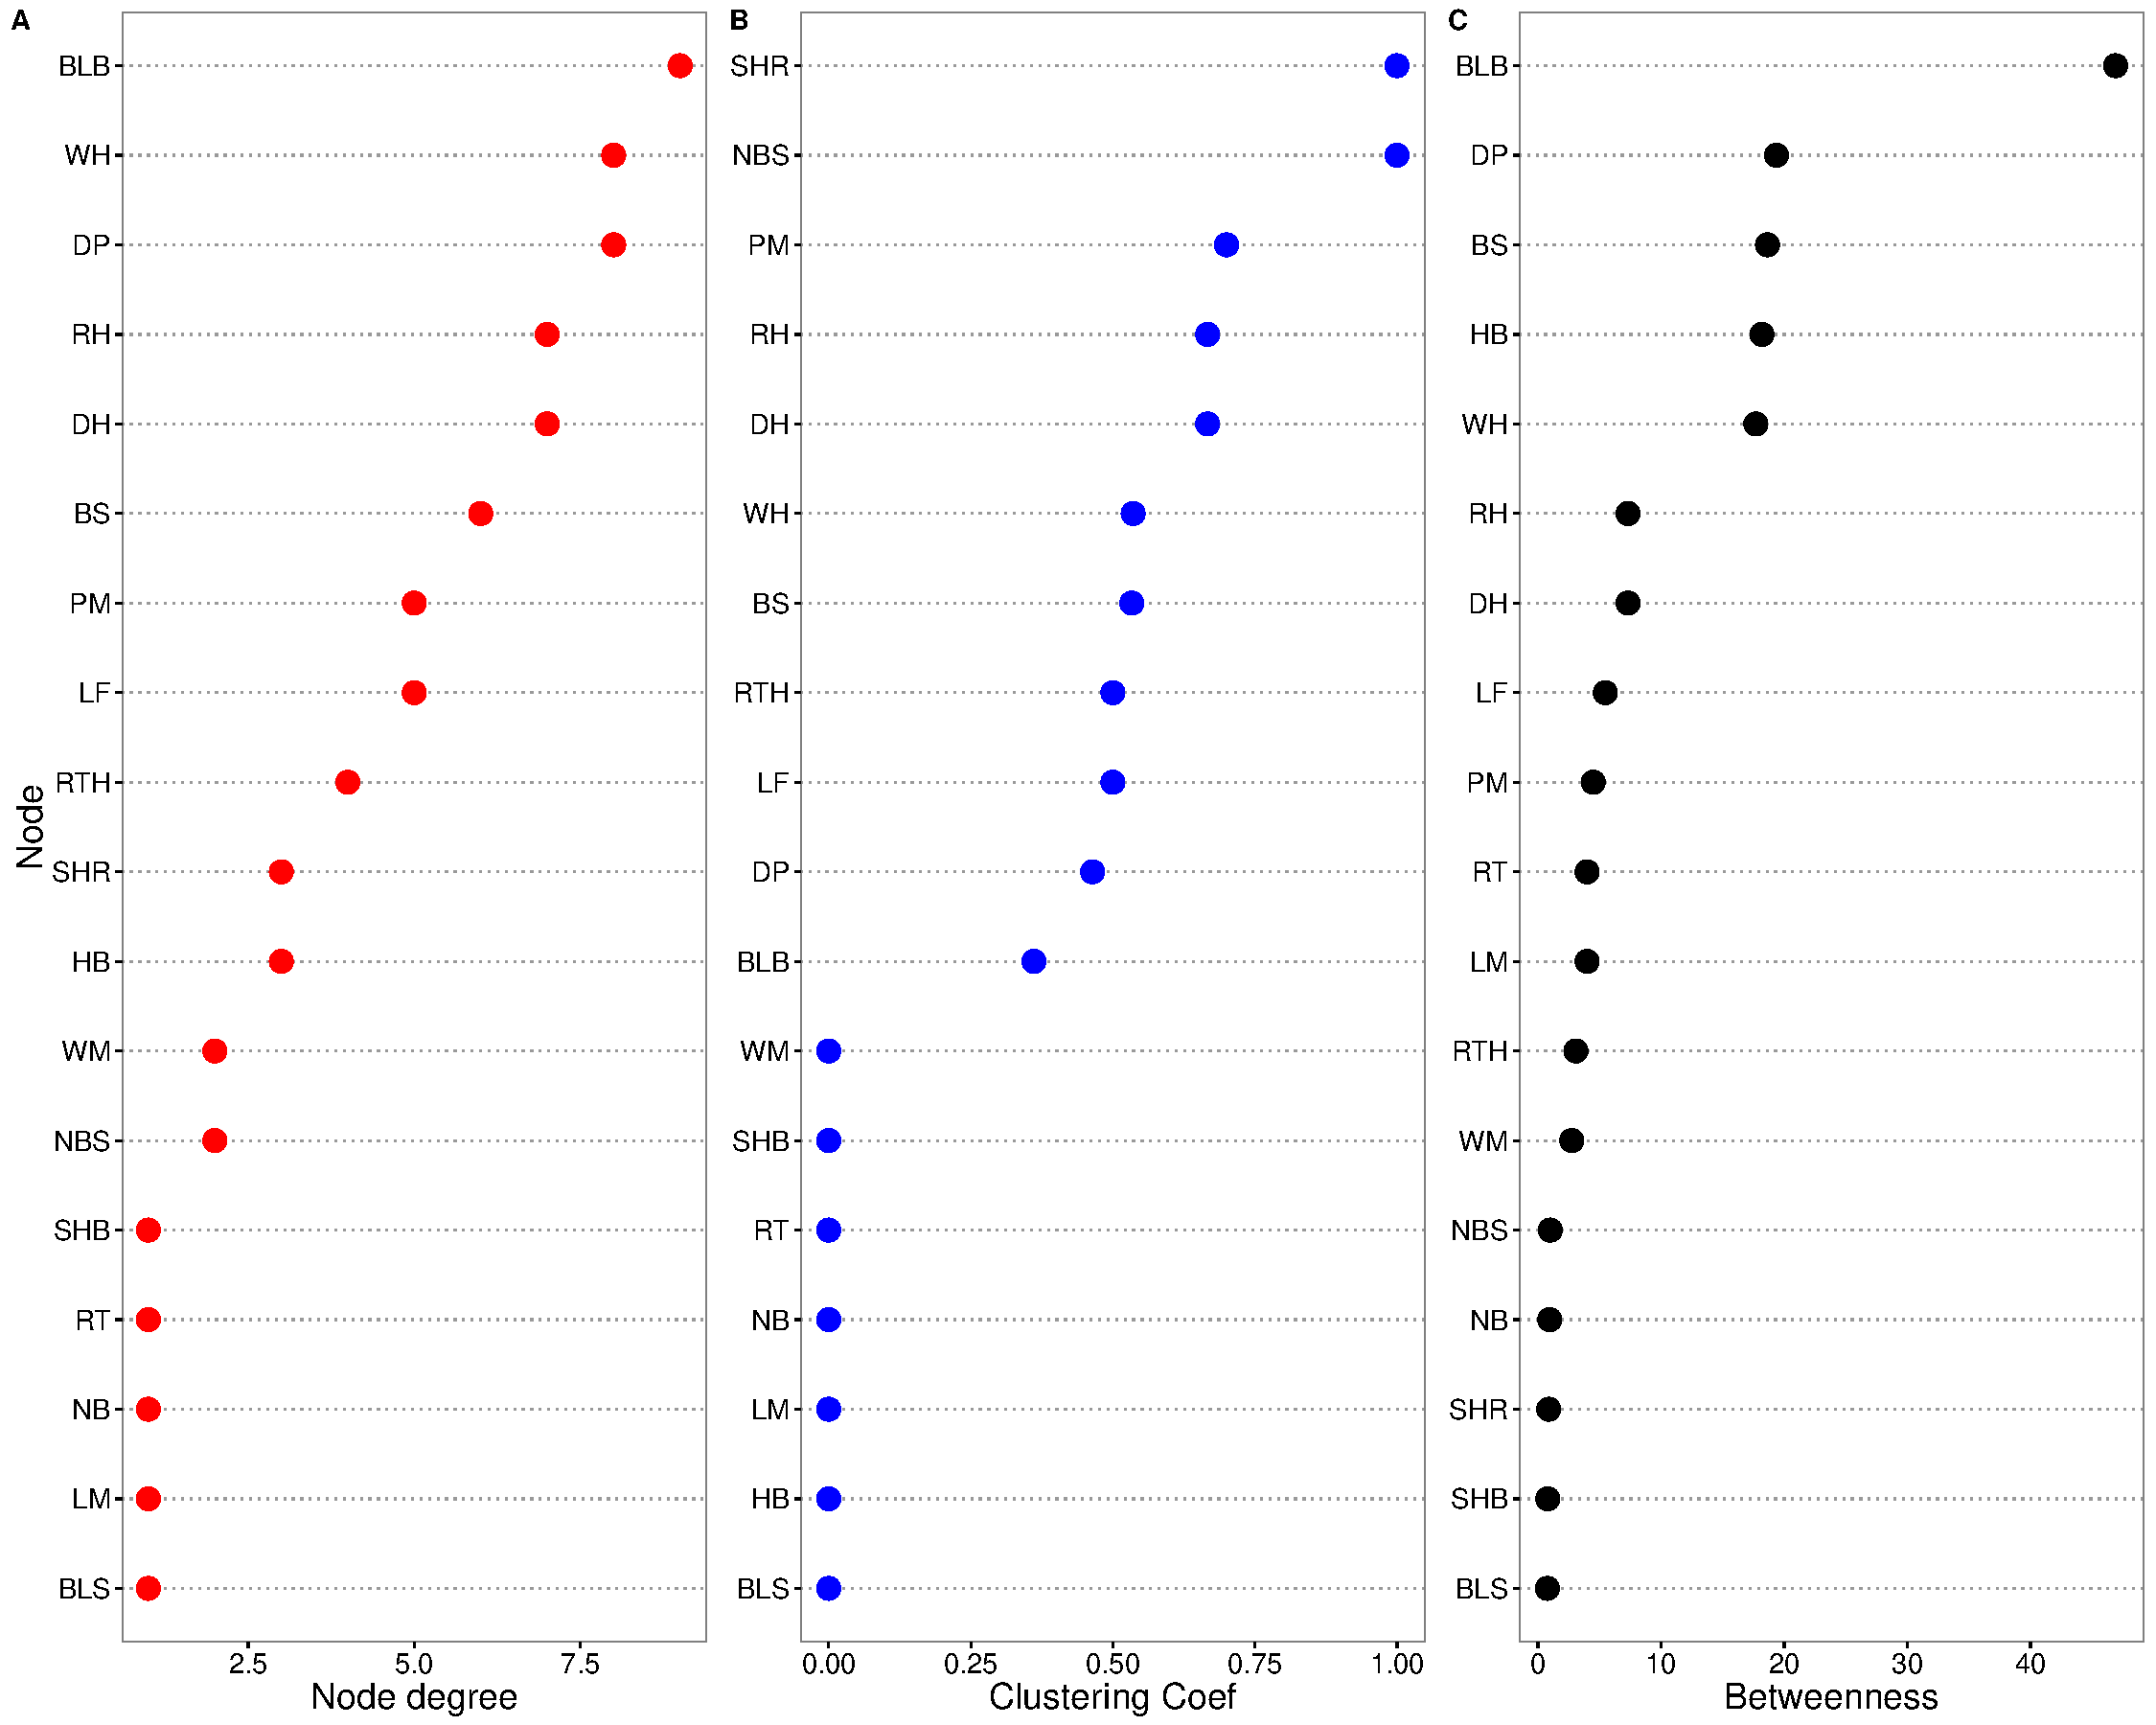
\includegraphics[width = 1\textwidth]{figures/nodepropRR_ws/nodepropRR_ws.pdf}
        \caption{Three centrality measures of the nodes in co-occurrence network of rice injuries in wet season at Red River Delta, Vietnam. A: node degree, B:clustering coefficient, and C:Betweenness}
        \label{fig:nodepropRR_ws}
    \end{subfigure}
    \caption{Network analysis of rice injury co-occurrence in wet season at Red River Delta, Vietnam}
    \label{fig:RR_ws}
\end{figure}


\textbf{Tamil Nadu, India}

The dry season network (Fig \ref{fig:networkTM_ds}) reveals three clustered groups of injury profiles. One of them is separated from other two. Syndrome1 is clustered tightly, which differ from group2 that injuries are placed further. SHB and BLB are disconnected to the rest. BS and WH highly tend to occur in this season (high betweenness) and are good indicators for monitoring in this season. Because clustering coefficient value of members in syndrome2 less than group1 (Fig \ref{fig:nodepropTM_ds}), injuries in syndrome2 might occur together with one or two more injuries. 

Figure \ref{fig:networkTM_ws} presents co-occurrence network of injury profiles in dry season. The network shows three syndromes related. Syndrome2 and syndrome 3 are linked with WH, and HB. NB is less possibly occur in this season because of low value of centrality measures. WH, RT can be good indicators because of high value of node degree and betweenness (Figure \ref{fig:nodepropTM_ws}). 

\begin{figure}
    \centering
    \begin{subfigure}[b]{1\textwidth}
        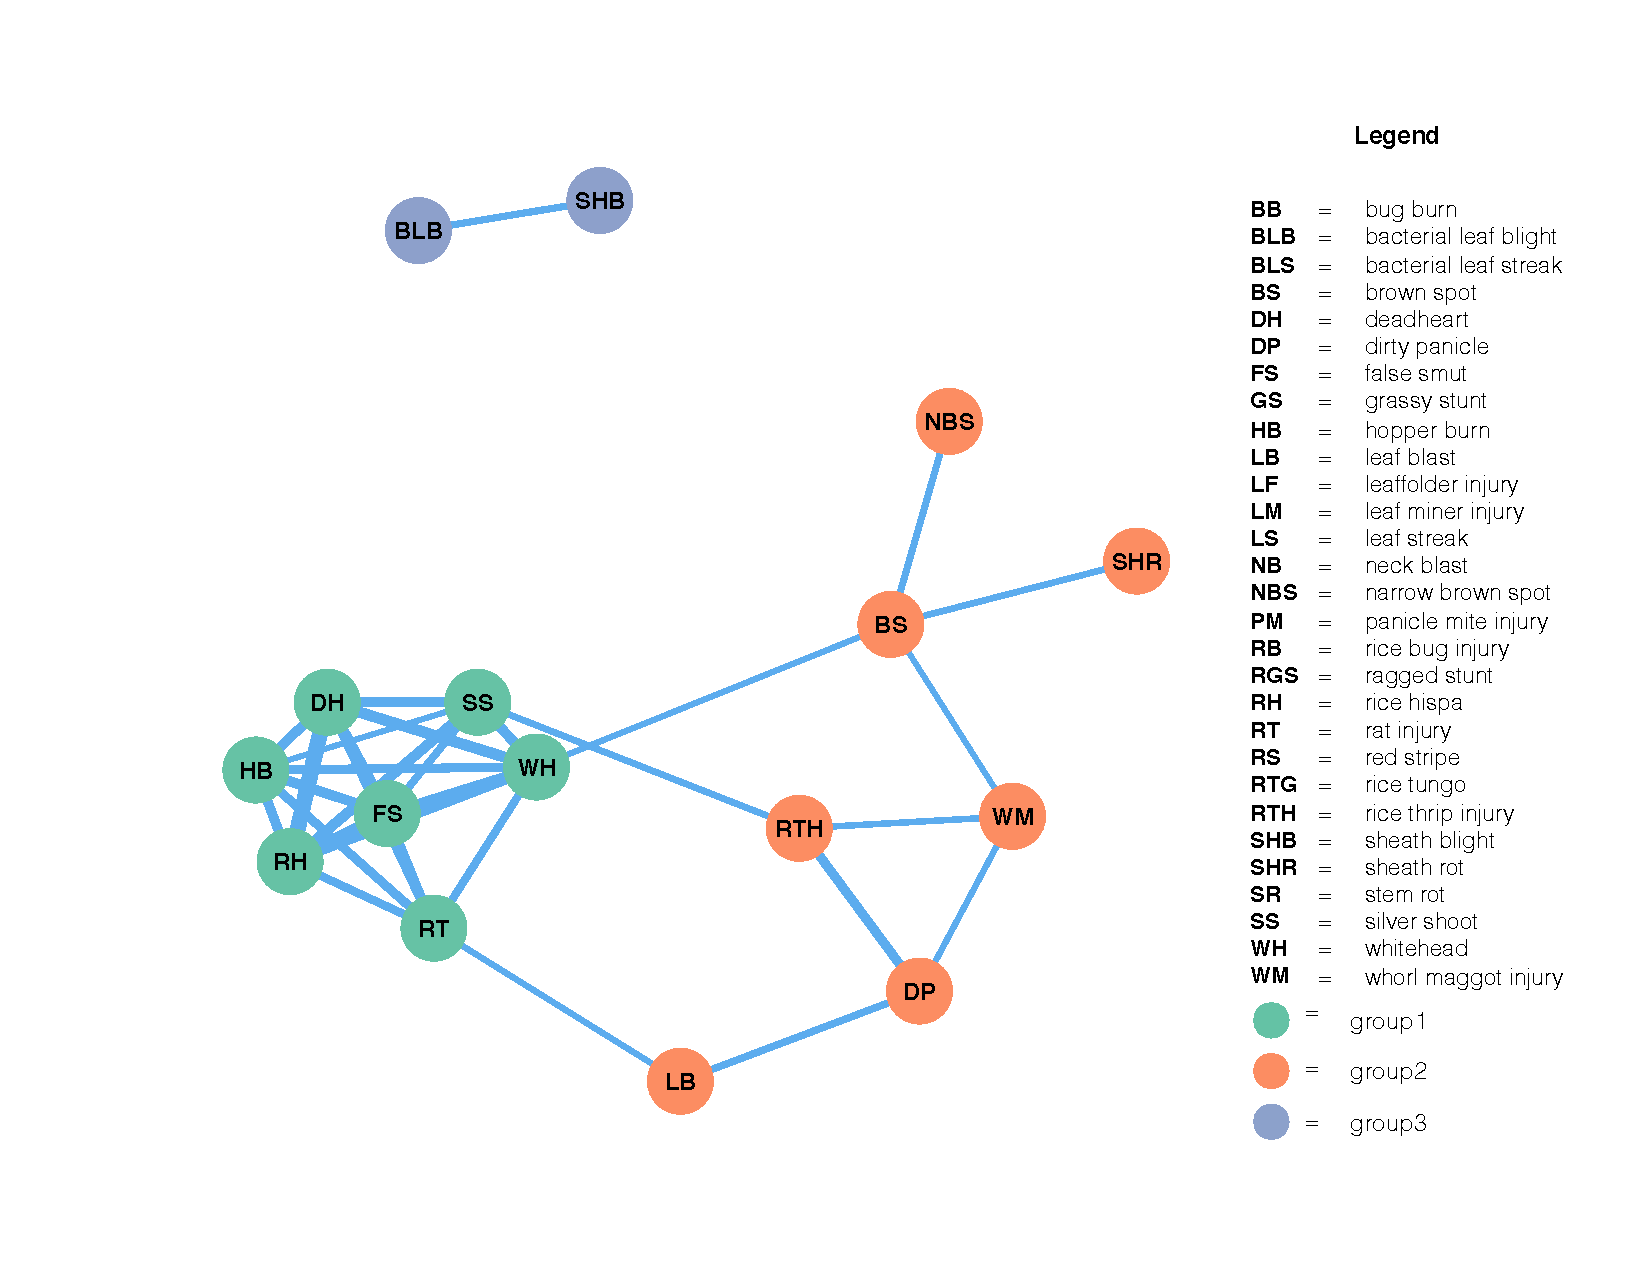
\includegraphics[width = 1\textwidth]{figures/networkTM_ds/networkTM_ds.pdf}
        \caption{Co-occurrence network of rice injuries in dry season at Tamil Nadu, India. The layout of the network graph is based on the Fruchterman-Reingold algorithm, which places nodes with stronger or more connections closer to each other.}
        \label{fig:networkTM_ds}
    \end{subfigure}
    \begin{subfigure}[b]{1\textwidth}
        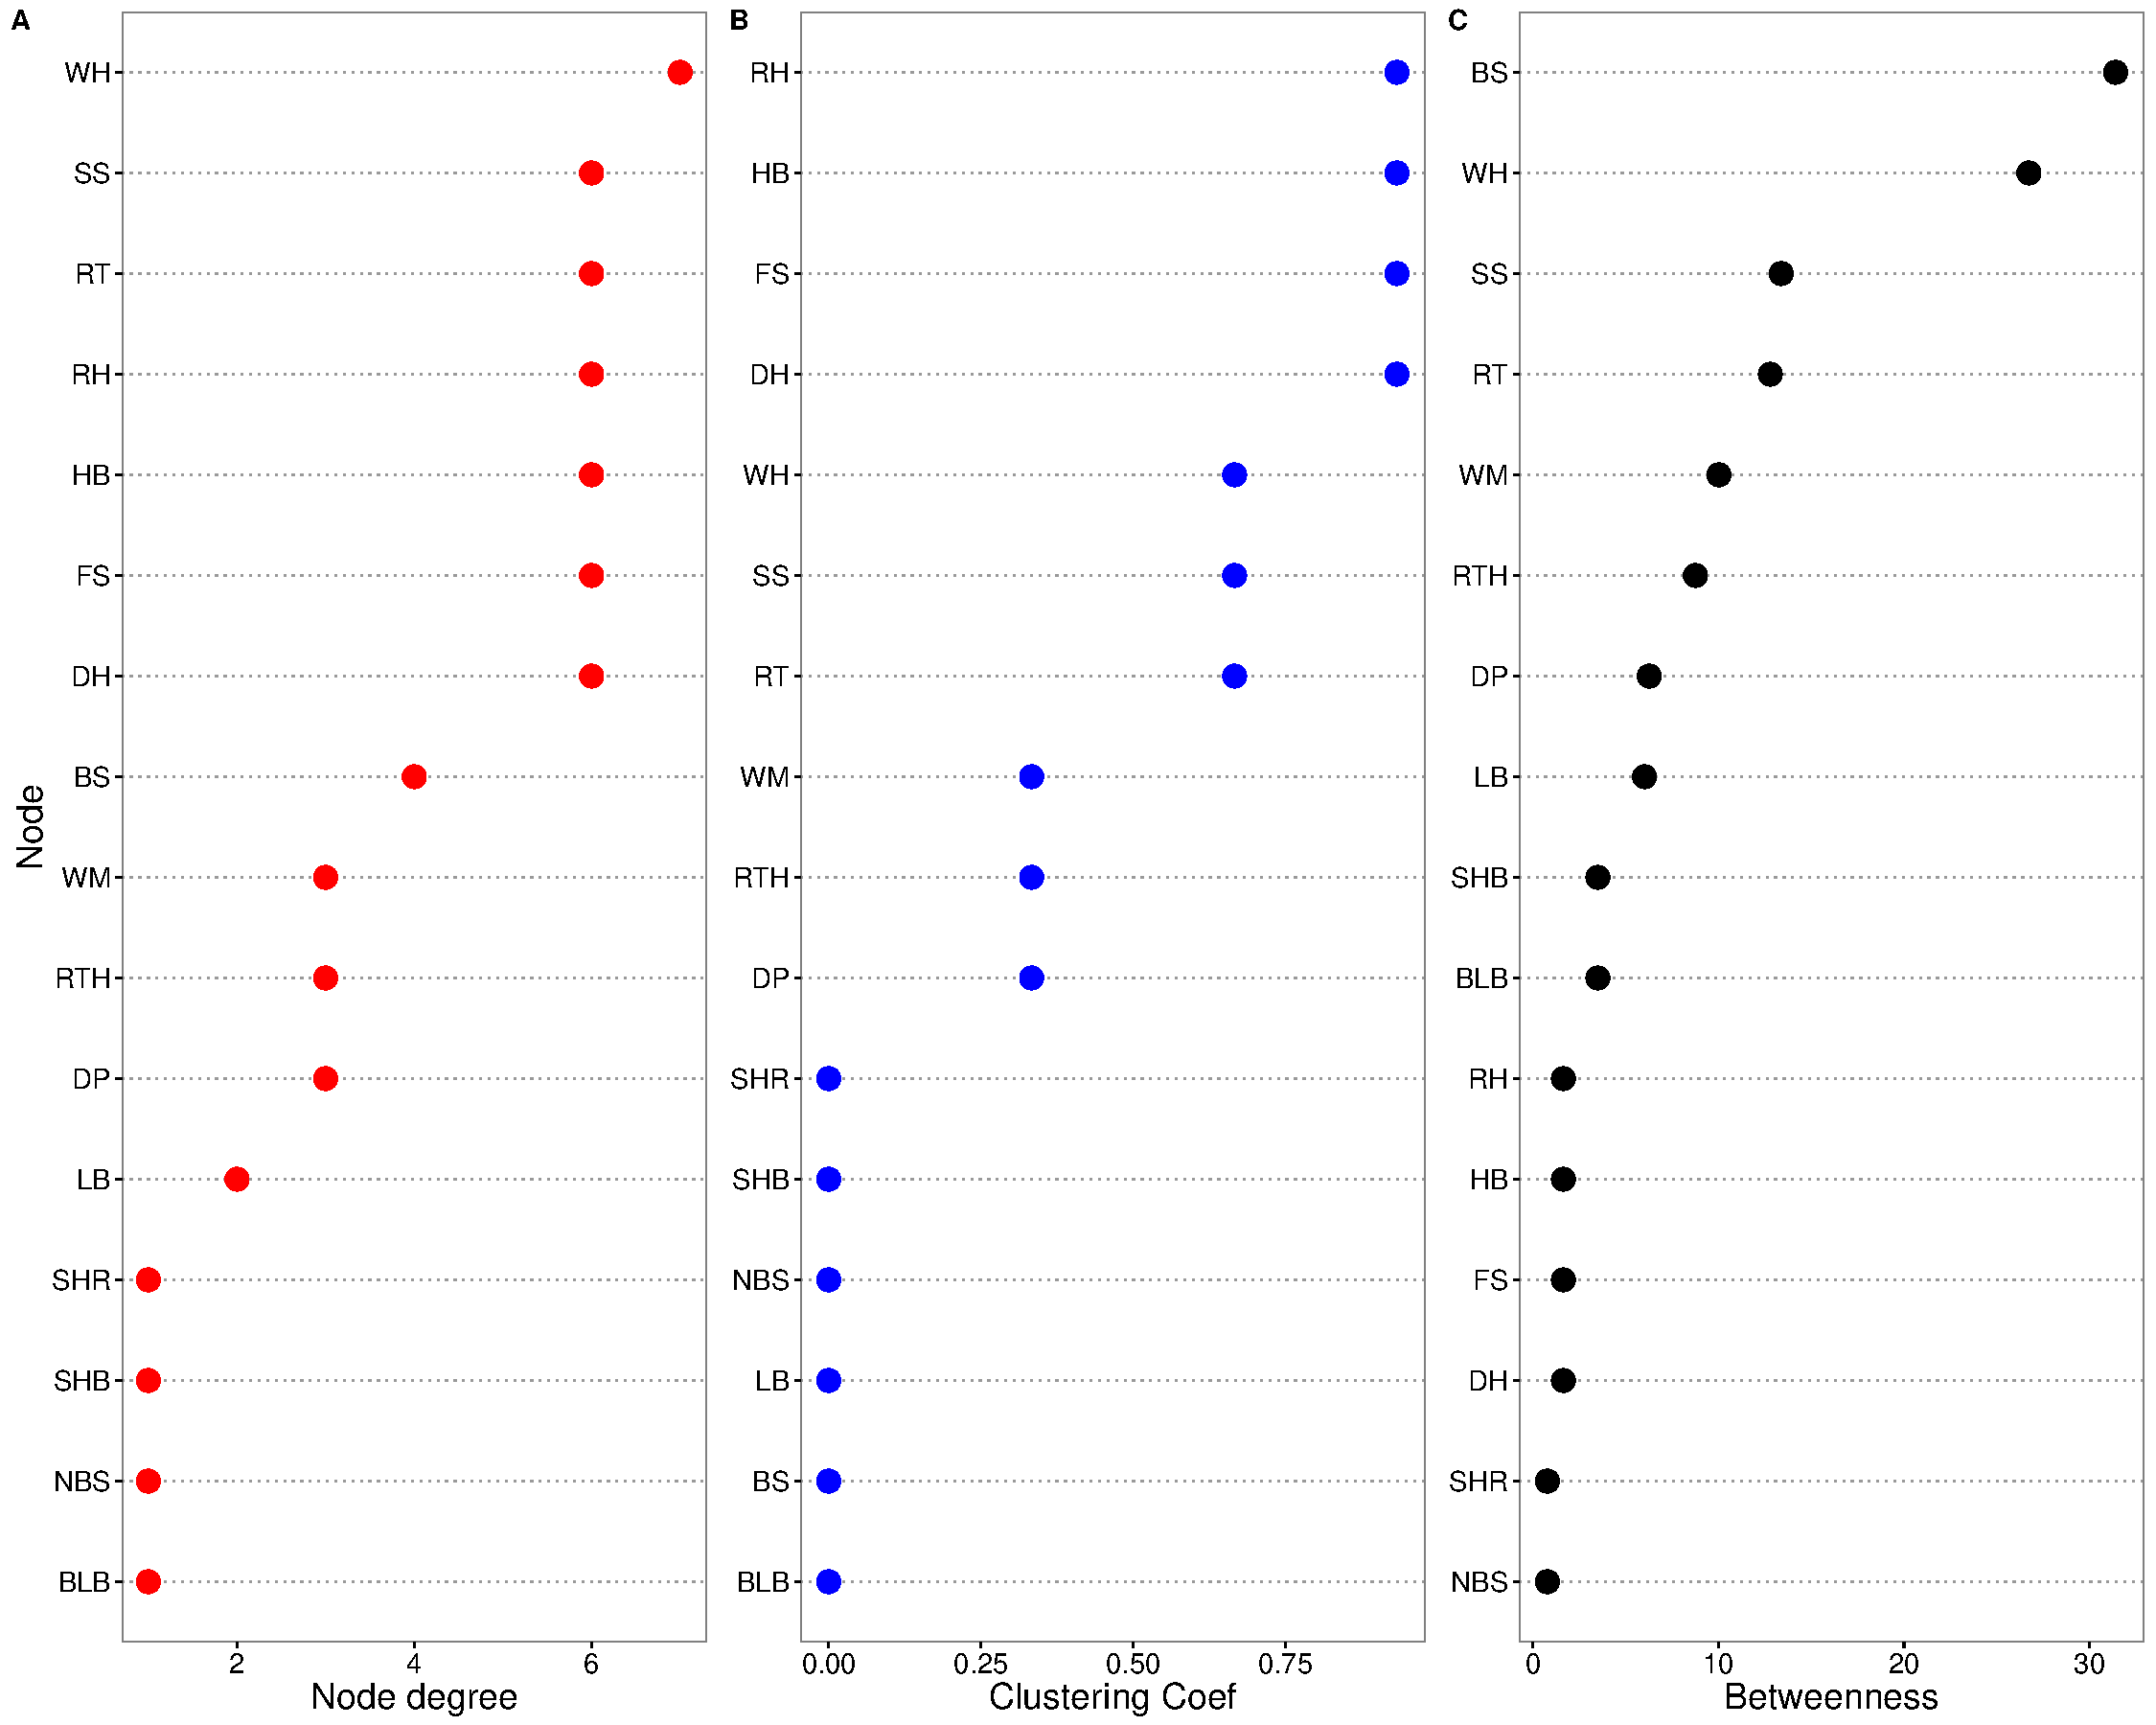
\includegraphics[width = 1\textwidth]{figures/nodepropTM_ds/nodepropTM_ds.pdf}
        \caption{Three centrality measures of the nodes in co-occurrence network of rice injuries in dry season at Tamil Nadu, India. A: node degree, B:clustering coefficient, and C:Betweenness.}
        \label{fig:nodepropTM_ds}
    \end{subfigure}
    \caption{Network analysis of rice injury co-occurrence in dry season in Tamil Nadu, India}
    \label{fig:TM_ds}
\end{figure}

\begin{figure}
    \centering
    \begin{subfigure}[b]{1\textwidth}
        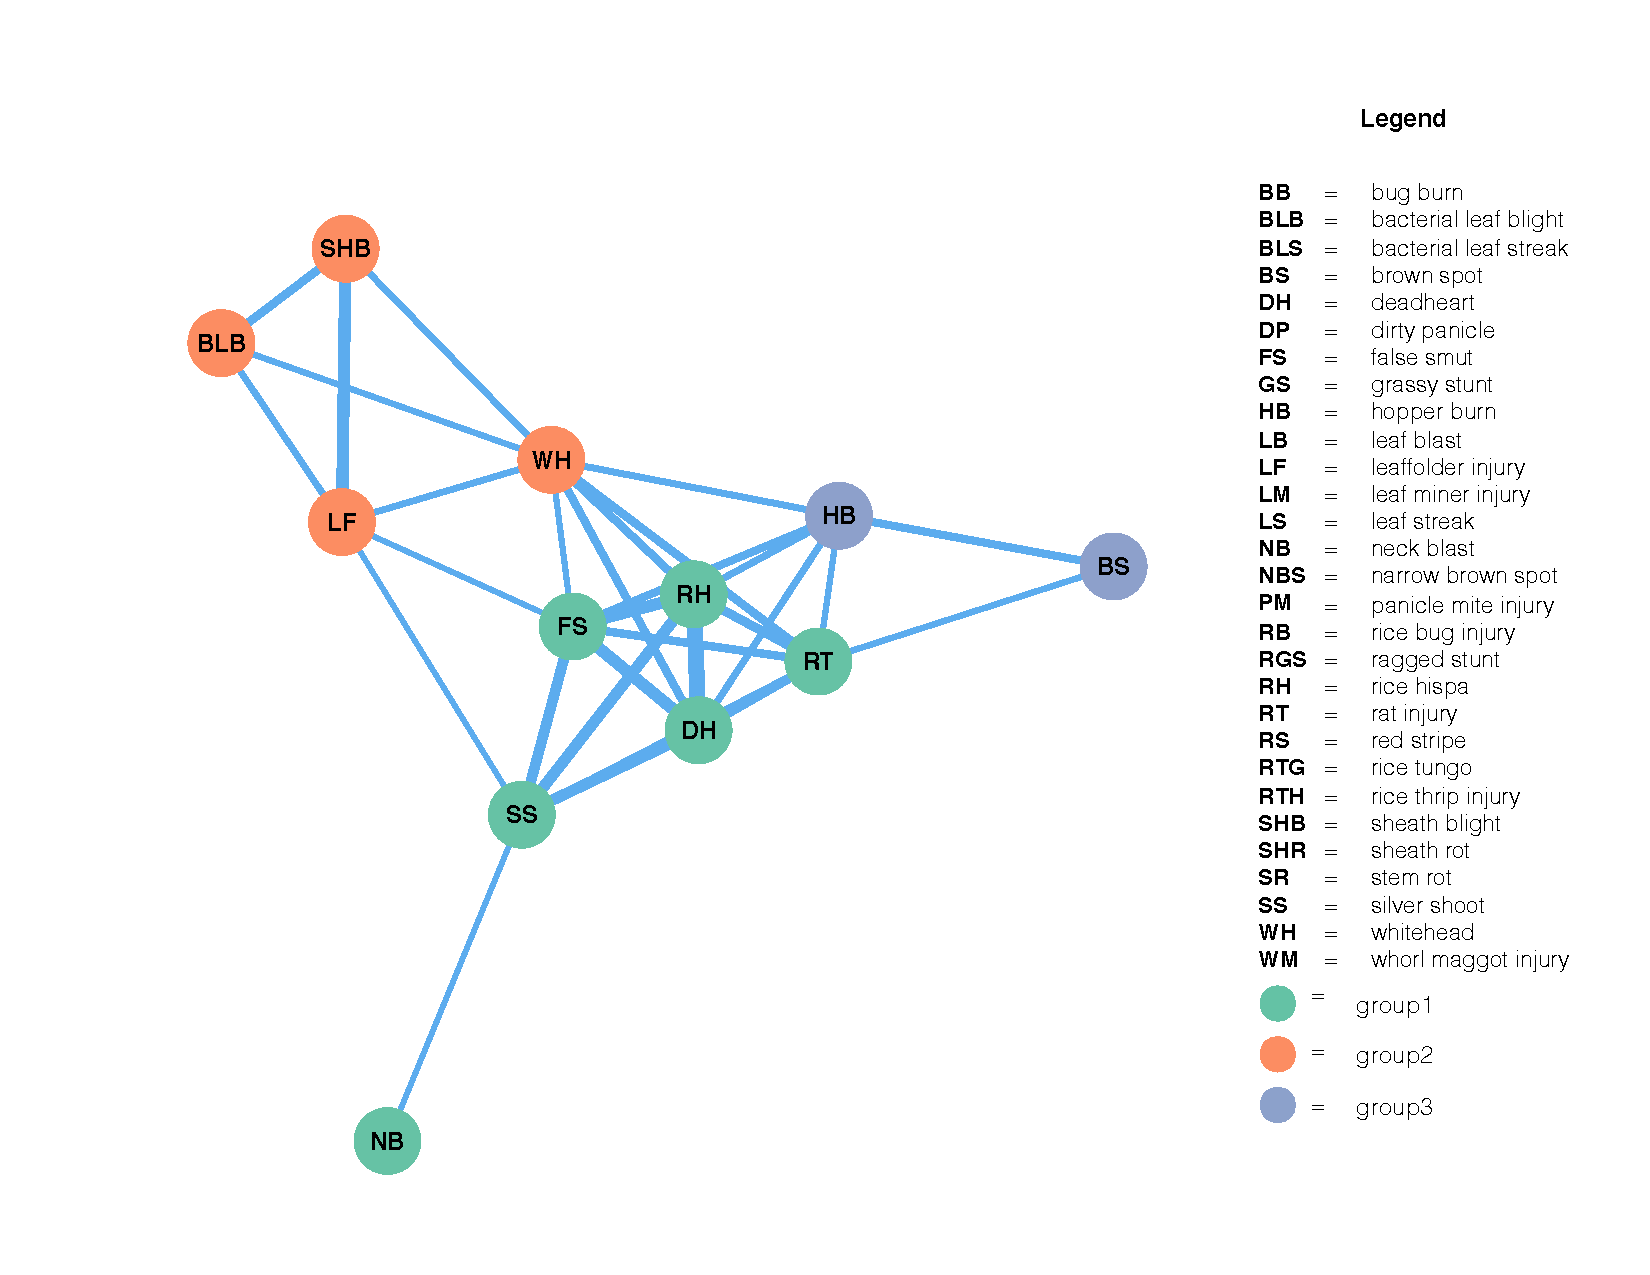
\includegraphics[width = 1\textwidth]{figures/networkTM_ws/networkTM_ws.pdf}
        \caption{Co-occurrence network of rice injuries in wet season at Tamil Nadu, India. The layout of the network graph is based on the Fruchterman-Reingold algorithm, which places nodes with stronger or more connections closer to each other.}
        \label{fig:networkTM_ws}
    \end{subfigure}
    \begin{subfigure}[b]{1\textwidth}
        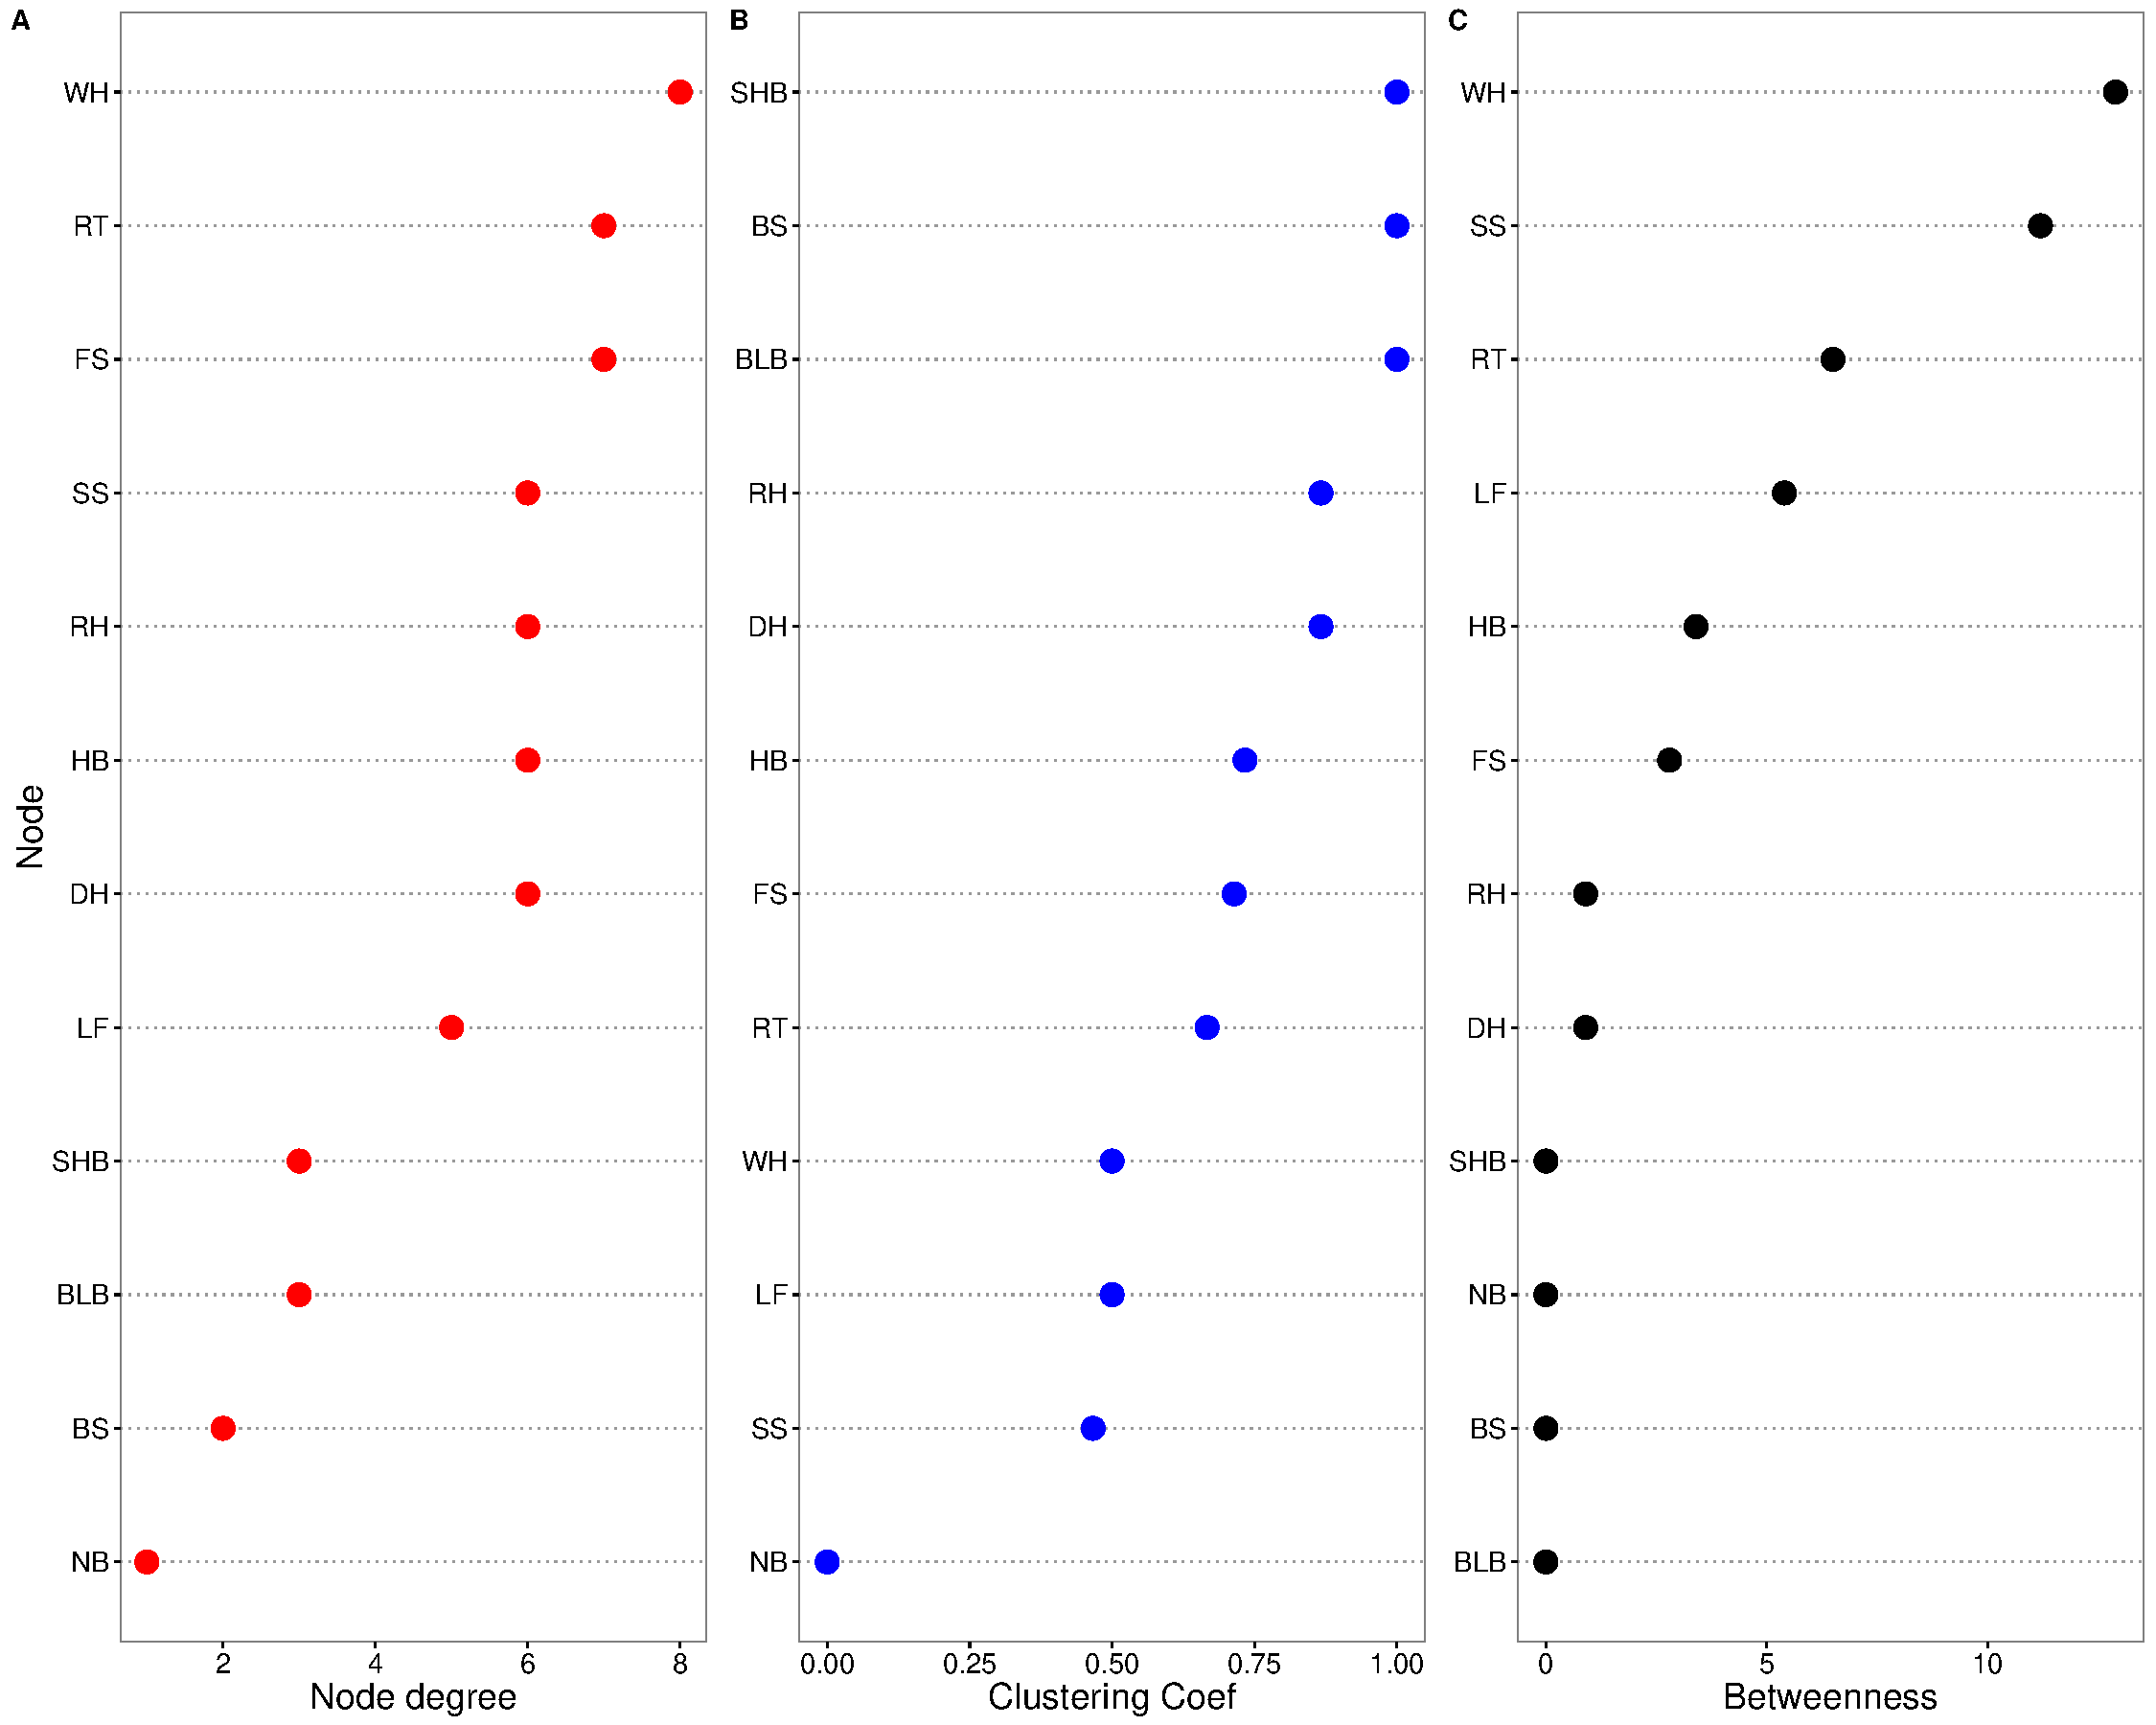
\includegraphics[width = 1\textwidth]{figures/nodepropTM_ws/nodepropTM_ws.pdf}
        \caption{Three centrality measures of the nodes in co-occurrence network of rice injuries in wet season at Tamil Nadu, India. A: node degree, B:clustering coefficient, and C:Betweenness.}
        \label{fig:nodepropTM_ws}
    \end{subfigure}
    \caption{Network analysis of rice injury co-occurrence in wet season at Tamil Nadu, India}
    \label{fig:TM_ws}
\end{figure}

\textbf{West Java, Indonesia}

Co-occurrence network of injury profiles of dry season presented in Figure \ref{fig:networkWJ_ds} showing 26 injury nodes and 99 association. High number of pest injuries and disease could be observed in dry season.  The network reveals the four syndromes of injury profiles. syndrome1 (green) and syndrome3 were close and syndrome2 and syndrome4 had less connection than others. Because of the structure and clustering coefficient, syndrome1 and syndrome3 are more likely to have chance to form complex association to each other. DH and RH of syndrome2 only related to BB of group1 and BS of syndrome3 but not to any of syndrome4. RT has smallest vales of all centrality measures. It indicated RT incidence is independent to other injuries.  According to Figure \ref{fig:nodepropWJ_ds}, LM, BS and NB can be good indicators for monitoring pest and disease incidence in this season.

The co-occurrence network of injuries of wet season (Figure \ref{fig:networkWJ_ws}) shows 14 injuries and 18 associations. Compared to the network of dry season the numbers of pest injuries and diseases in wet season are less. The network structure reveals three types of injury syndromes. Syndrome1 (green) composed of SHB, RT, DH, RH, BLS, and SHR.  Within this group, BLS and SHB seem to be good indicator (high betweenness and high node degree) according to Figure \ref{fig:nodepropWJ_ws}. Syndrome2 (orange) seems to be the panicle or tiller injury syndrome because there is the combination of PM, RB, and FS. Apparently, within this combination, BS is center of association, and early occur among other injuries. All of injuries in syndrome3 (purple), which is combination of BS, LF, WM, NBS, and LM are leaf injures. 

\begin{figure}
    \centering
    \begin{subfigure}[b]{1\textwidth}
        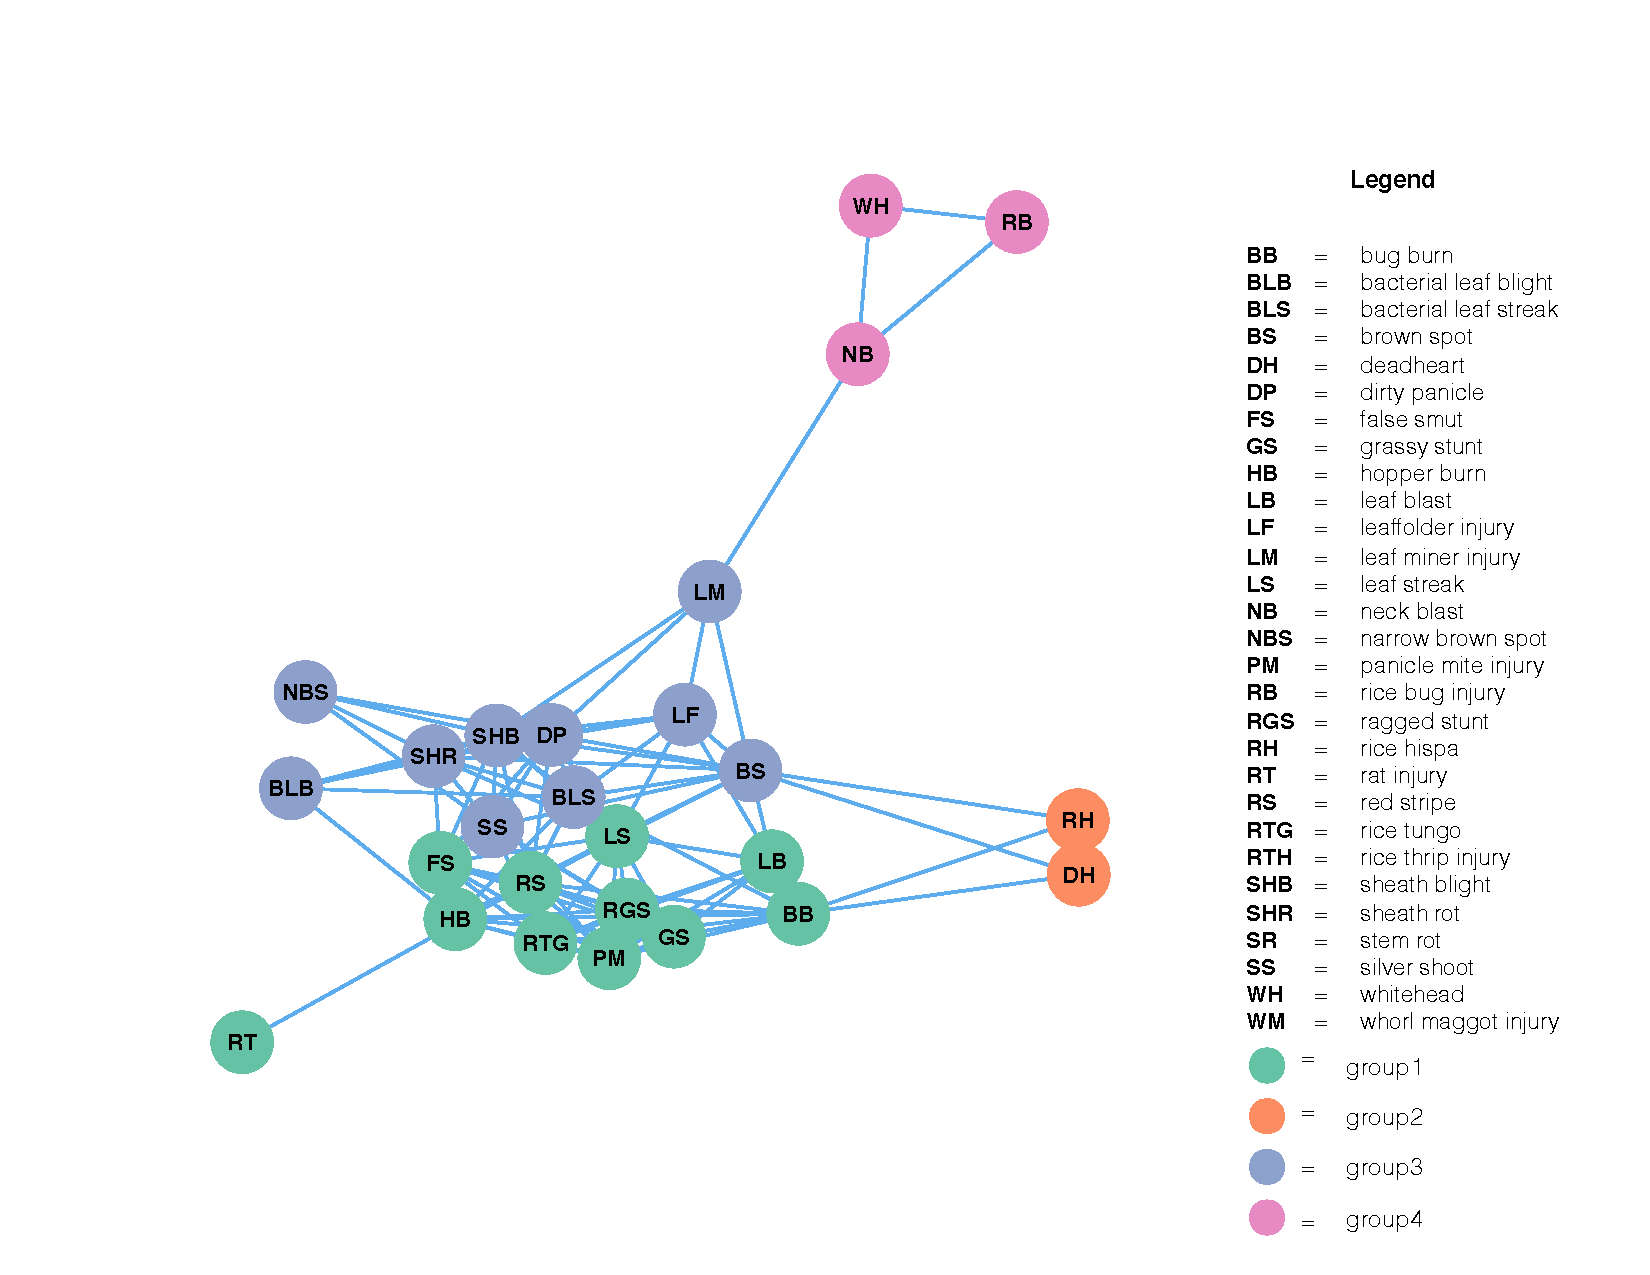
\includegraphics[width = 1\textwidth]{figures/networkWJ_ds/networkWJ_ds.pdf}
        \caption{Co-occurrence network of rice injuries in dry season at West Java, Indonesia. The layout of the network graph is based on the Fruchterman-Reingold algorithm, which places nodes with stronger or more connections closer to each other.}
        \label{fig:networkWJ_ds}
    \end{subfigure}
    \begin{subfigure}[b]{1\textwidth}
        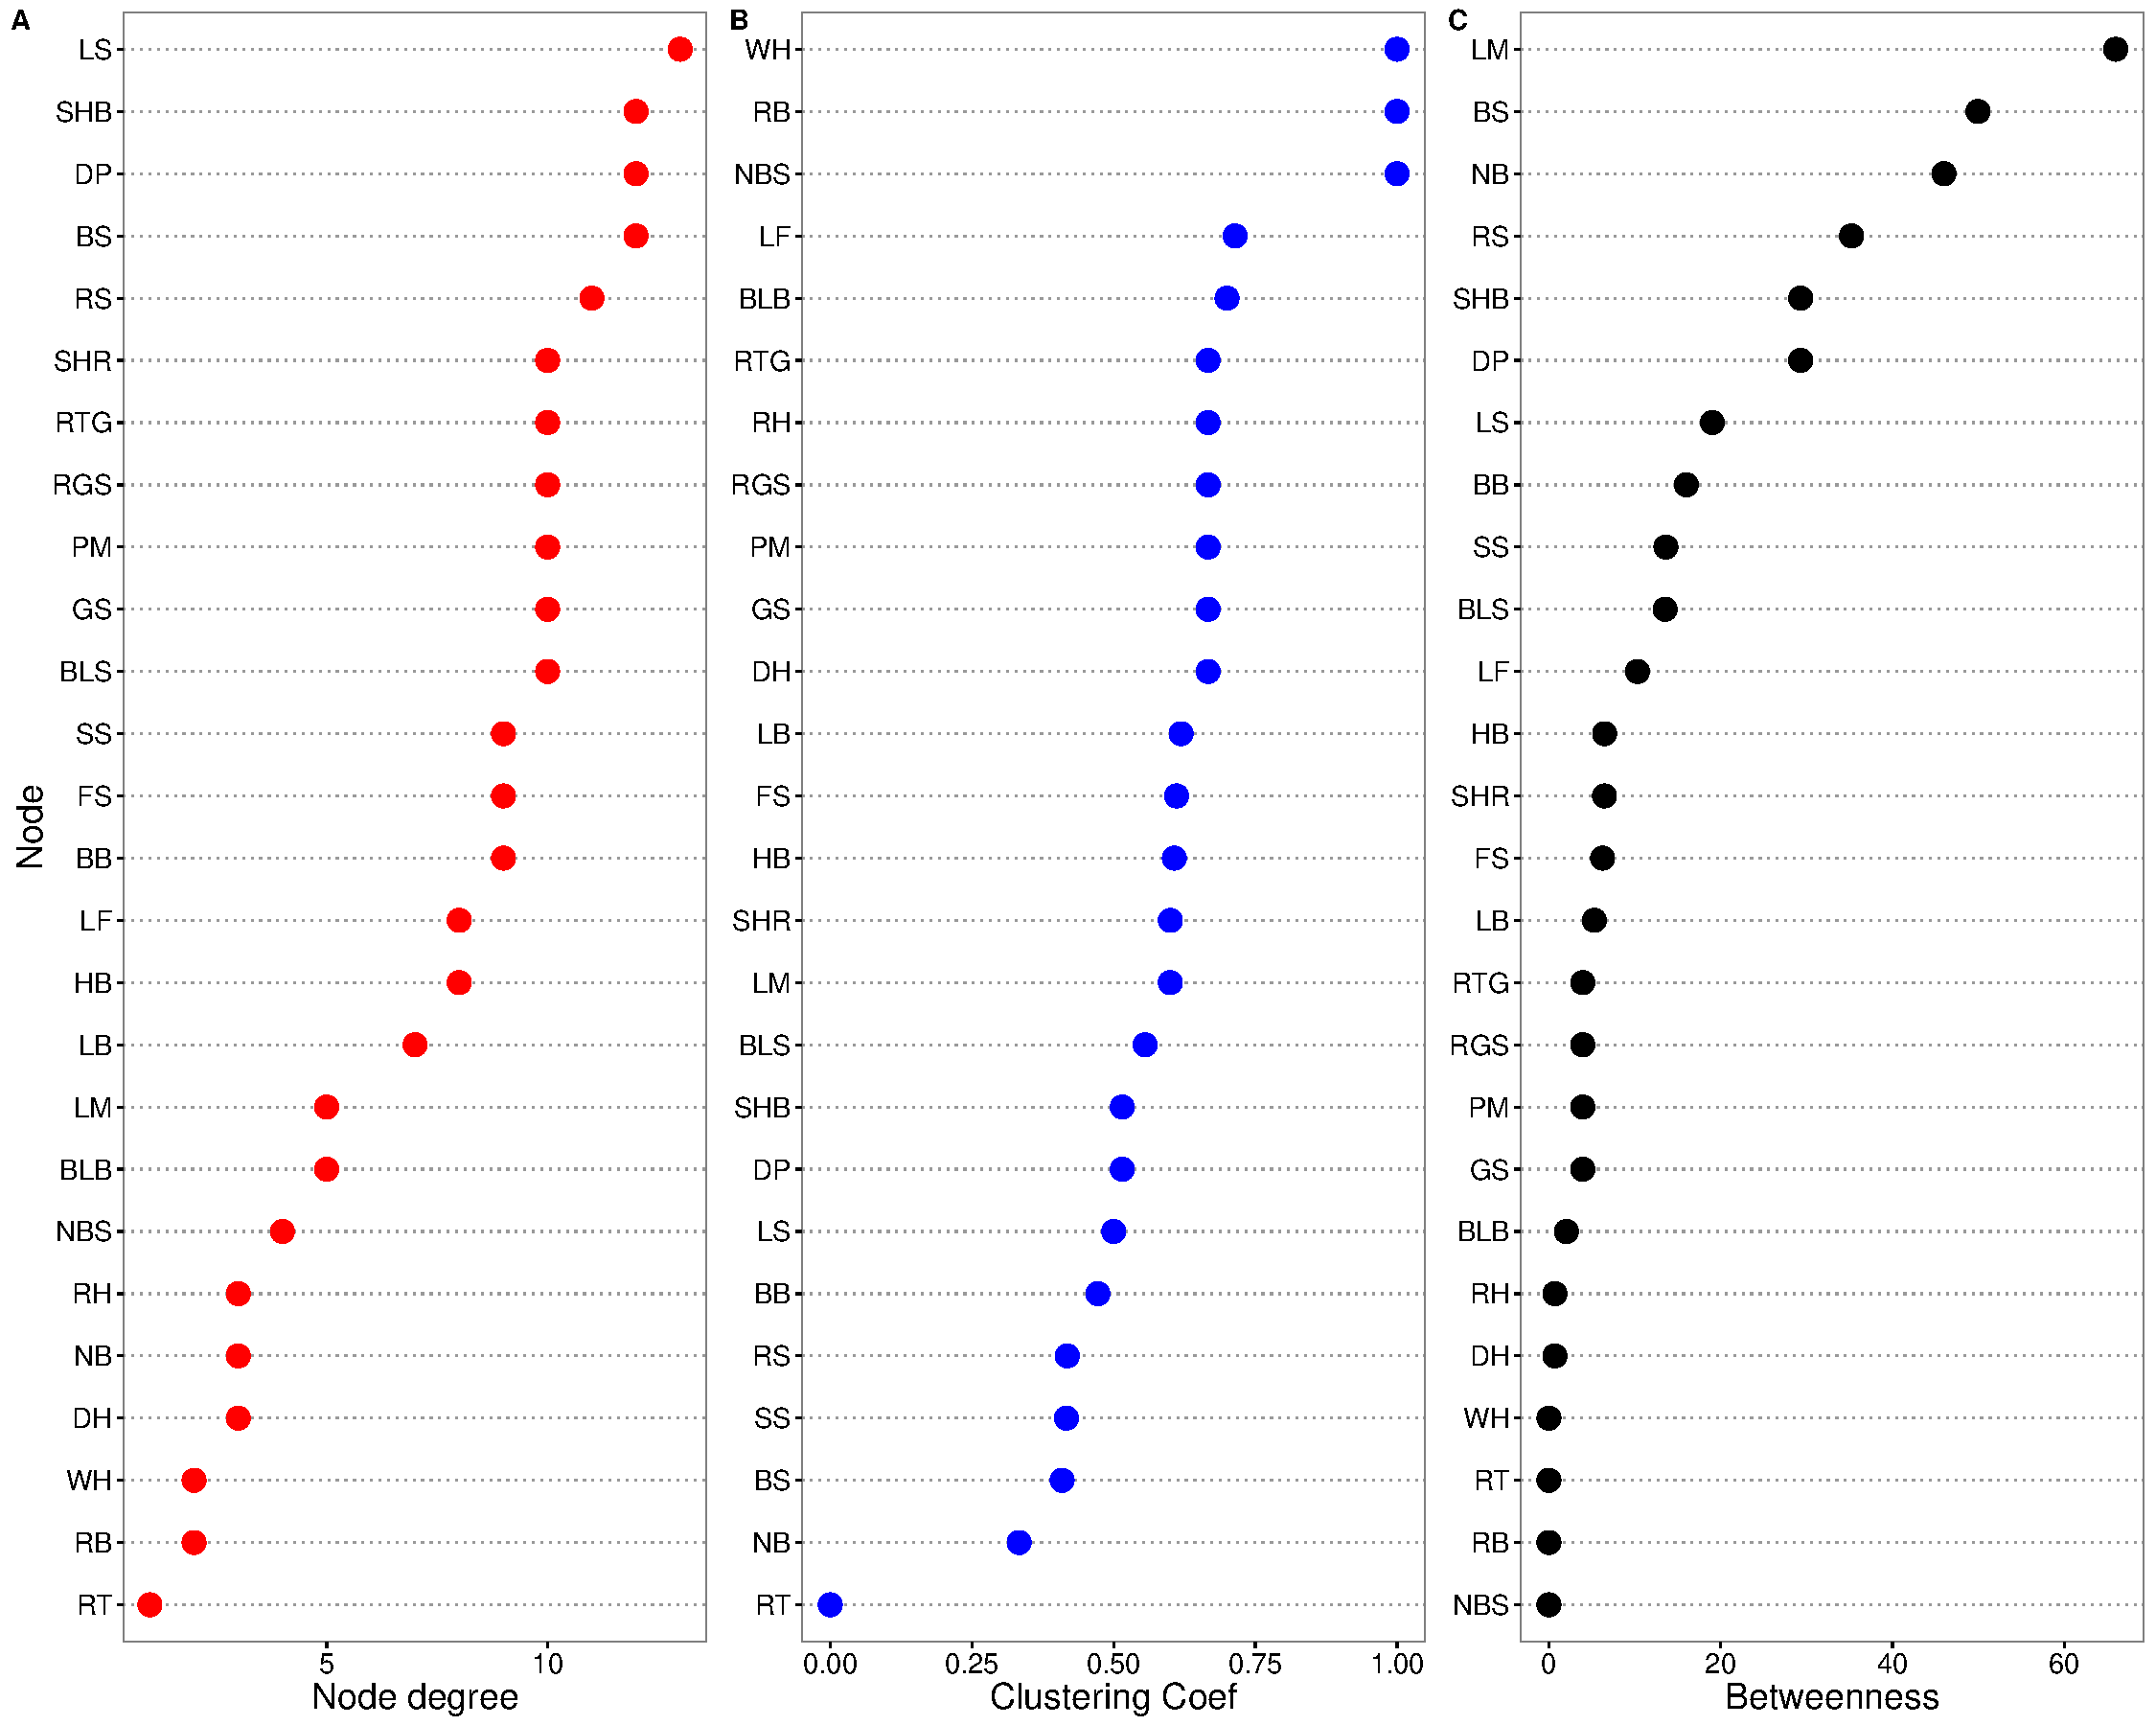
\includegraphics[width = 1\textwidth]{figures/nodepropWJ_ds/nodepropWJ_ds.pdf}
        \caption{Three centrality measures of the nodes in co-occurrence network of rice injuries in dry season at West Java, Indonesia. A: node degree, B:clustering coefficient, and C:Betweenness.}
        \label{fig:nodepropWJ_ds}
    \end{subfigure}
    \caption{Network analysis of rice injury co-occurrence in dry season at West Java, Indonesia}
    \label{fig:WJ_ds}
\end{figure}

\begin{figure}
    \centering
    \begin{subfigure}[b]{1\textwidth}
        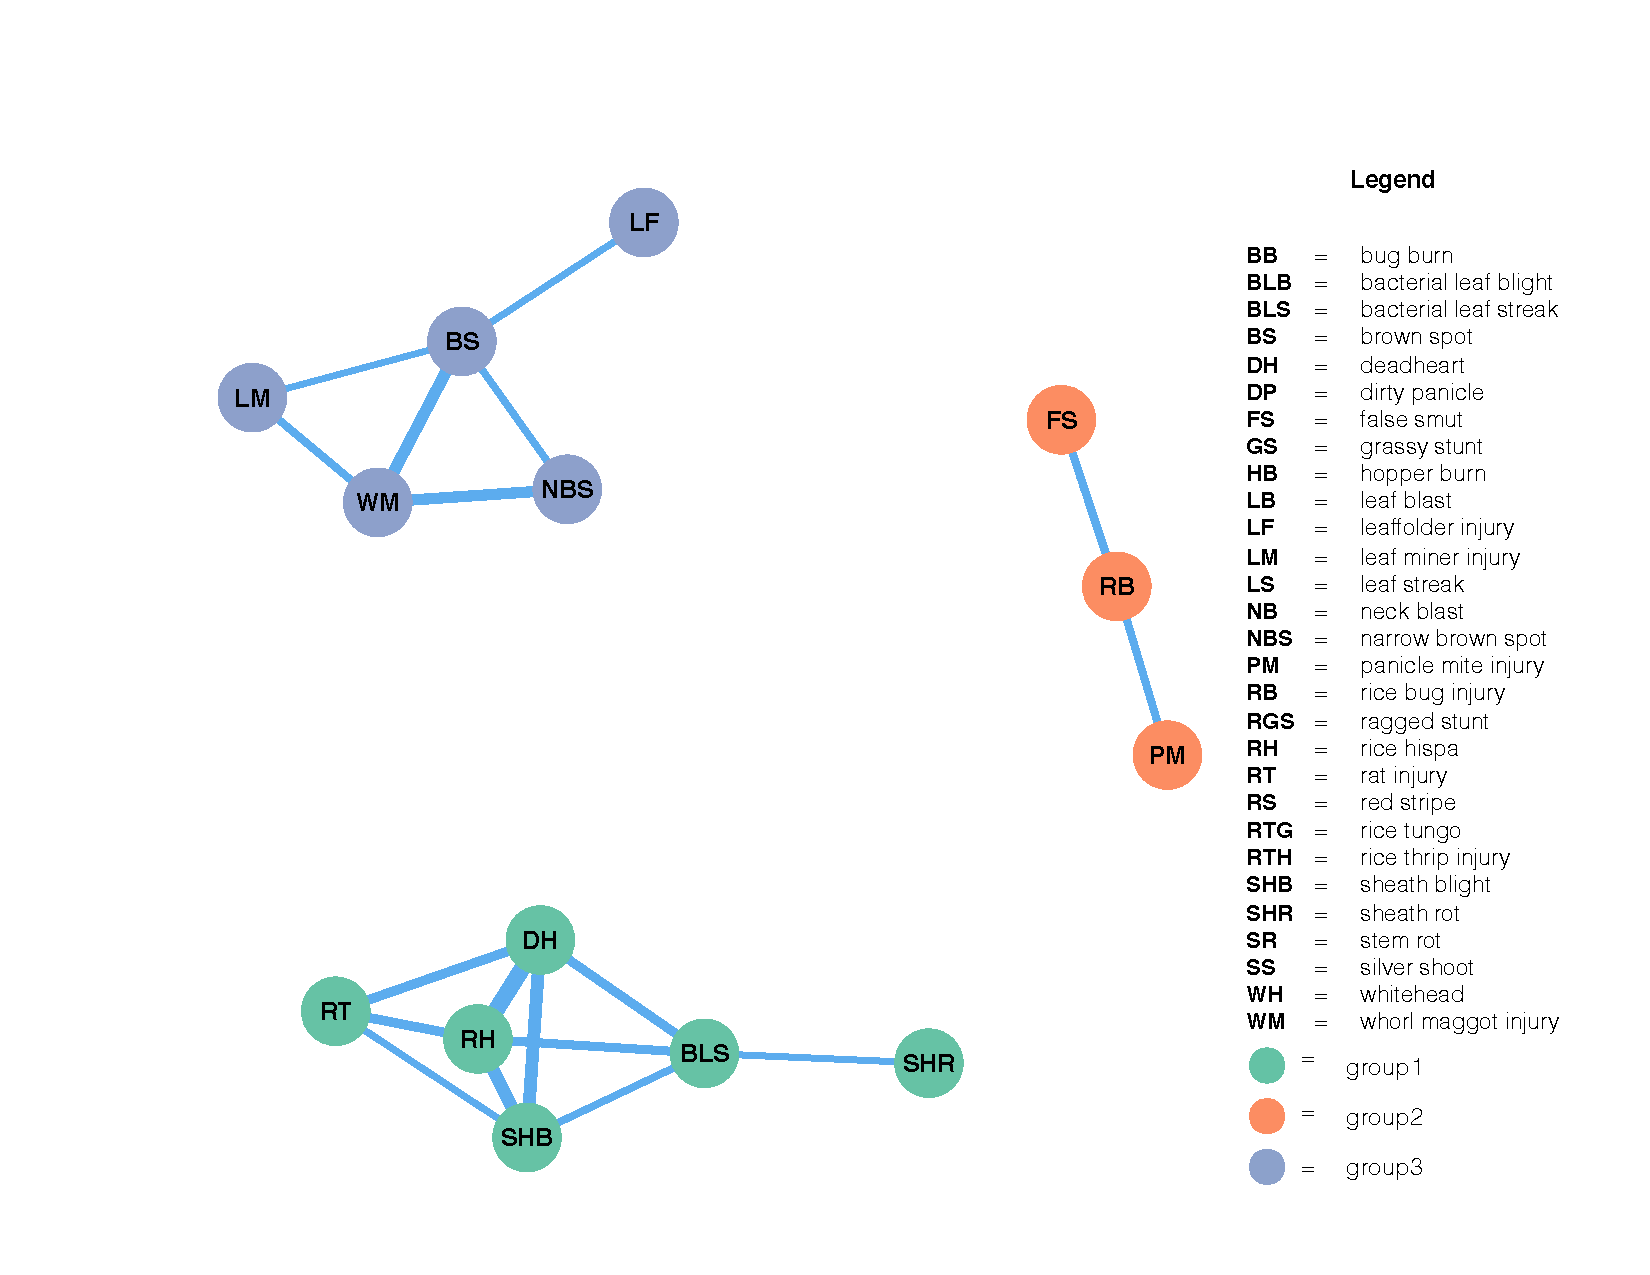
\includegraphics[width = 1\textwidth]{figures/networkWJ_ws/networkWJ_ws.pdf}
        \caption{Co-occurrence network of rice injuries in wet season at West Java, Indonesia. The layout of the network graph is based on the Fruchterman-Reingold algorithm, which places nodes with stronger or more connections closer to each other.}
        \label{fig:networkWJ_ws}
    \end{subfigure}
    \begin{subfigure}[b]{1\textwidth}
        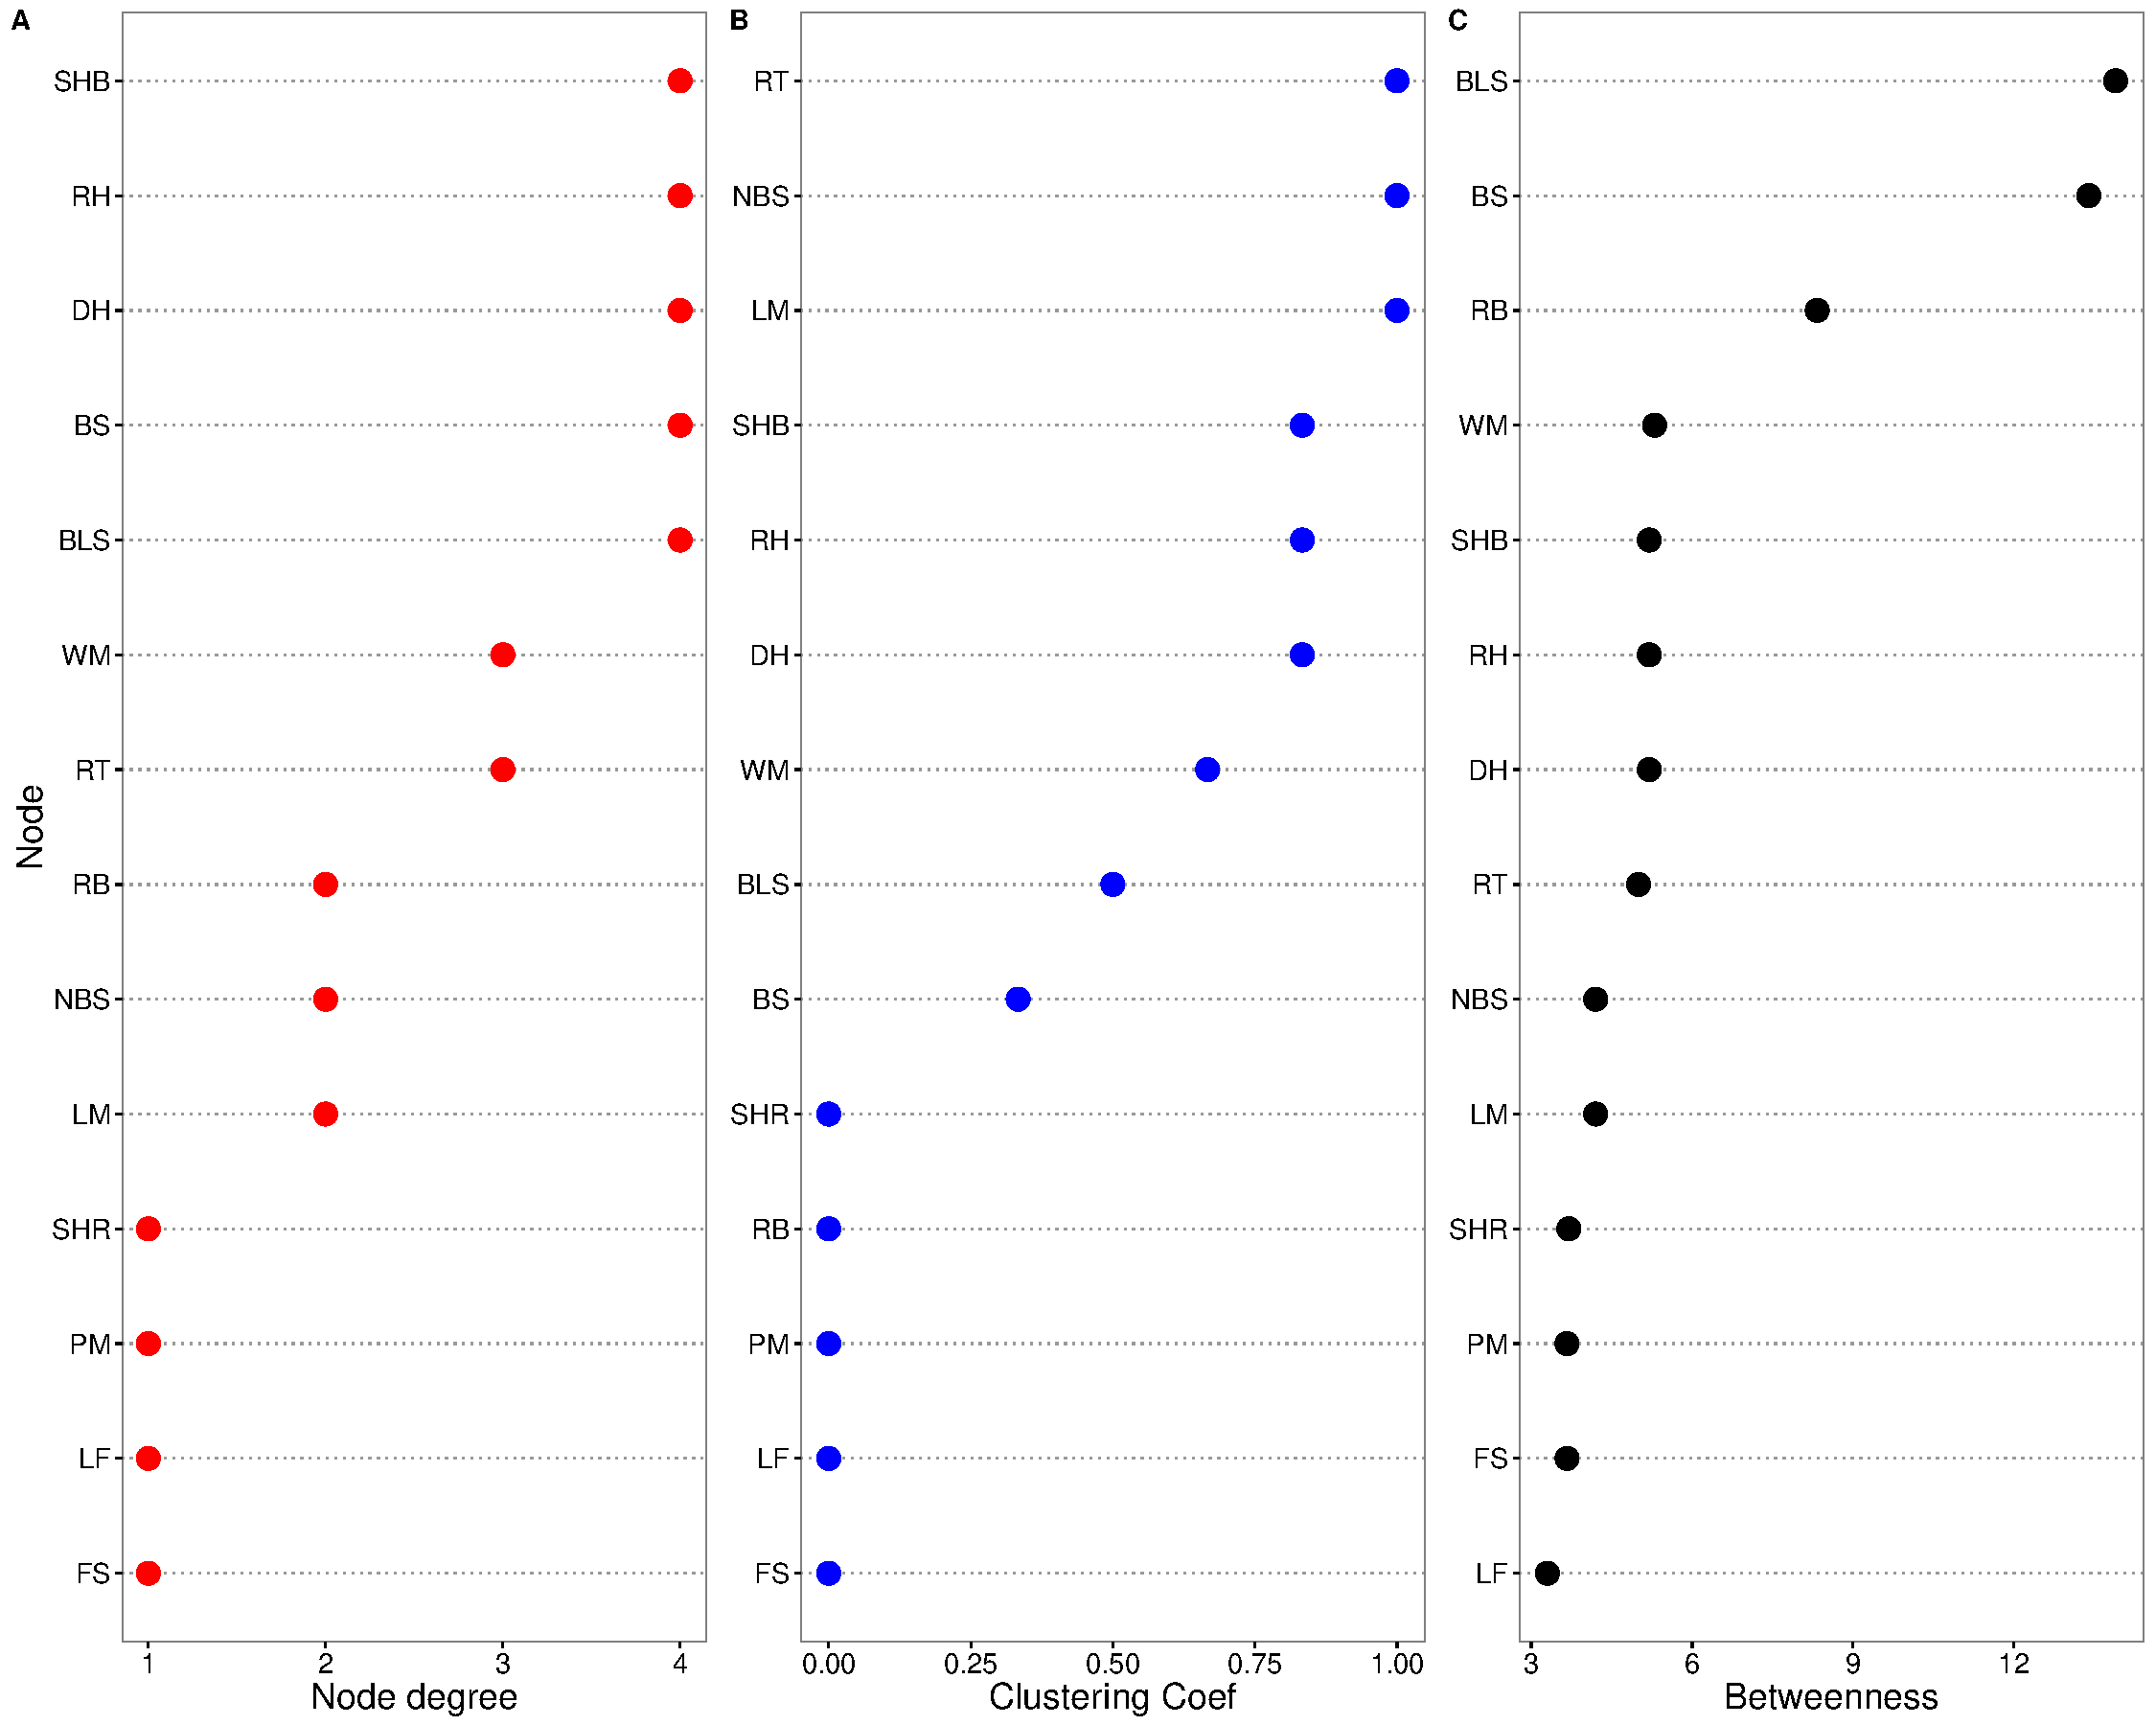
\includegraphics[width = 1\textwidth]{figures/nodepropWJ_ws/nodepropWJ_ws.pdf}
        \caption{Three centrality measures of the nodes in co-occurrence network of rice injuries in wet season at West Java, Indonesia. A: node degree, B:clustering coefficient, and C:Betweenness.}
        \label{fig:nodepropWJ_ds}    \end{subfigure}    
\caption{Network analysis of rice injury co-occurrence in wet season at West Java, Indonesia}
    \label{fig:WJ_ws}
    \end{figure}


\newpage
\subsection{Discussion}
% Survey data
Rice injuries caused by animals, and pathogens were found commonly in South and South east Asia, but at different levels of incidence. Injuries indeed depended on locations or climate conditions favorable to develop \citep{Savary_2006_Quantification}. So they were not observed at all production environments or season during survey were conducting. For example, red stripe was often found in Central Plain, and West Java in dry season. 

The co-occurrence correlations of rice injuries were explored using network inference based on strong and significant correlations through using non-parametric Spearman’s rank coefficient. Usually, correlations were assessed using Pearson correlation. However, the use of the Pearson correlation coefficient is problematic because it requires the variables are applied with similar measure, and the variable values are normally distributed. Additionally, Pearson correlation can only capture linear relationships. Due to the fact that the assumptions of Pearson correlation are not fit with the survey data. The alternative is provided by using Spearman’s rank correlation coefficient, which is also widely used in biological, and ecological studies
  
The exploration of co-occurrence networks is a useful method for determining interactions of co- occurring injuries. The centrality of nodes is considered further. The node centrality is the identification of which nodes are ``central’’ than others \citep{Barrat_2004_Architecture}. \citet{Newman_2003_Structure} mentioned three measures of node centrality: node degree, clustering coefficient, and betweenness. The node degree is measured by the number of connections a node has. In co-occurrence networks of rice injuries, node degree of each injury was counted from the number of the positive relationships of injuries have with other injuries. The clustering coefficient measure a density of local connectivity. Higher clustering coefficient of an element, the higher is the relationship among their neighbors. In the context of theses co-occurrence networks, nodes with high clustering coefficients were located closely. This indicated that they strongly occur together; one increasingly occurred, the related one also occurred jointly. In biological network, betweenness is used for measuring has been of how central a node is in a network, because a node with high betweenness essentially play an important role as a bridge between different parts of the network \citep{Proulx_2005_Network, Newman_2010_Networks}. In this study, nodes with high betweenness could be represented as indicators. Because theses nodes have many connections passed through, they are likely to be induced, and have higher chance to occur before other injuries associated.

Peripheral nodes or low-centrality nodes are also interesting. Ecological studies considered theses nodes as specialists that have a few links and link specially to curtain nodes \citep{Lu_2013_Soil, Borthagaray_2014_Inferring}. In the context of co-occurrence networks of injuries, peripheral nodes have a few relationships within their groups in the network. They also slightly depend on other injuries. This may imply that these injuries are difficult to control because they may occur occasionally such as rat injury (RT) in dry season at West Java, Indonesia, neck blast (NB) in wet season, in Tamil Nadu, bacterial leaf streak (BLS) in Red River Delta, bacterial leaf blight (BLB), rat injury (RT) and sheath blight (SHB) in wet season at Odisha, India.

Nodes display high betweenness are suggested that these nodes have important roles in regulating network interactions such as key stone species in ecological network \cite{Wright_2012_Microbial}. It can illustrate both the number of connections and how important those connections are to the overall network. Therefore, in the co-occurrence network, I identified injury indicators, which are the injuries are highly sensitive to the favorable conditions for the associated injuries in the networks. For example, in wet season at West Java, the network showed that brown spot is a good indictor of syndrome3, which is comprised of leaf miner injury, whorl maggot injury, narrow brown spot, and leaffolder injury. Compared to other injuries within this group, brown spot shared association to all the injuries, then brown spot potentially can be observed earlier under a curtain condition. When we first found brown spot, there is high chance that related injuries will occur. 

It was found that the co-occurrence networks of rice injuries changed with seasons and production environments. The same injuries in the network would connect to different injuries as the change of seasons and production environments. In according with previous findings \citep{Savary_2000_Characterization, Avelino_2006_Intensity, Savary_2012_Review} , the pest and disease syndromes (combination of pest injuries and diseases) are strongly associated with climatic condition at regional scale. In Red River Delta, brown spot had relationships with sheath blight in dry season, but in wet season brown spot had association with bacterial leaf blight. 
  
Community structures in networks can reveal hidden information that is maybe not easy to detect by simple observation. In social studies, community detection has been applied to search the groups of people who are interested in same topics.   In this study, I detected node community based on the optimization of the modularity of a sub-network, which is a popular approach \citep{Liu_2014_Detecting}. Communities are groups that are densely connected among their members, and sparsely connected with the rest of the network. Community structure can reveal abundant hidden information about complex networks that is not easy to detect by simple observation. Communities in a co-occurrence network of rice injuries might represent the rice injury co-occurrence association under related conditions. For example, the network of dry season in Central Plain revealed that group2 (LB, WM, LF and BLB).  According to \citet{Savary_2000_Characterization}, these injuries were in injuries profile group2 (IN2). They also mentioned that IN2 was related to production situation group2 (PR2), this type was also dominantly found in direct seeded rice fields. So injuries in group2 of the network in dry season in CP could co-occur favorably in rice fields where applied direct seedling method, which is the most common practices in Thailand \citep{IRRI_2013_Rice}. 
\newpage
\subsection{Conclusion}

In order to establish priorities and strategies for pest management program, there is a need for characterization of multiple pests \citep{Mew_2004_Looking}. I applied network analysis to characterize co-occurrence patterns of rice injuries from crop health survey data, which were collected in farmers’ fields at five production environments (Central Plain; Thailand, Odisha; India, Red River Delta; Vietnam, Tamil Nadu; India, and West Java; Indonesia) across South and Southeast Asia for three consecutive years (2013-2015). The resulted networks depicted the co-occurrence patterns of rice injuries at different production seasons, and production environments. The networks revealed the different structure, which reflect to the co-occurrence patterns between injuries, in different production seasons and production environment. From the network structures, networks showed injury syndromes (groups of injuries) that are closely related in the network. Additionally, from three important of node centrality measures (node degree, clustering coefficient, and betweenness), I can identify indicators that are used for monitoring, and predict the trend that associated injuries to occur under a curtain condition that may be favorable for injury indicators. This information is useful to better understand the variation of rice injury occurrence, and to develop the more effective strategies of pest management specifically to seasons or production environments (locations).

%Important challenges, however; remain in order to further rice injury characterization:
%\begin{itemize}
%\item What are the rice injuries that occurred differently in season;
%\item at different yield levels, the patters of rice injury occurrence;
%\item differentiate the patterns for injuries at deferent production environments. 
%\end{itemize}


